%% ---------------------------------------------------------------------------
%%  A tempered analogue of Lemma 4(a) of Yang, Wainwright and Jordan (2016).
%%
%%  Notation is theirs throughout.  The only symbols introduced here are the
%%  inverse temperature lambda, the tempered posterior pi_n^(lambda), and the
%%  two temperatures lambda_star and lambda_crit that the results produce.
%%  No other quantity is given a name: every intermediate expression is
%%  written out, as they write it.
%%
%%  Self-contained.  Bibliography: bvs.bib.
%% ---------------------------------------------------------------------------
\documentclass[aos]{imsart}

\RequirePackage[authoryear]{natbib}
\RequirePackage{graphicx}

\usepackage{amsmath, amsfonts, amsthm, amssymb}
\usepackage{mathtools}
\usepackage{mathrsfs}
\usepackage{enumitem}
\usepackage{tikz}
\usepackage[colorlinks,citecolor=blue,urlcolor=blue,filecolor=blue]{hyperref}
\usepackage[capitalise]{cleveref}

\newlist{equivcond}{enumerate}{1}
\setlist[equivcond,1]{
    label=\normalfont\bfseries(\alph*),
    leftmargin=4em,
    noitemsep,
    ref=\alph*,
}

\startlocaldefs

\DeclarePairedDelimiter{\norm}{\lVert}{\rVert}
\DeclarePairedDelimiter{\abs}{\lvert}{\rvert}

\newcommand{\bbE}[0]{\mathbb{E}}
\newcommand{\bbR}[0]{\mathbb{R}}
\newcommand{\calN}[0]{\mathcal{N}}
\newcommand{\Ind}[0]{\mathbb{I}}
\newcommand{\opnorm}[1]{|\!|\!|#1|\!|\!|_{\mathrm{op}}}
\newcommand{\Ltil}{\widetilde{L}}

%% Typesetting shorthands only.  Each expands to the full expression, so the
%% reader never meets a new symbol; they exist to keep the source readable.
\newcommand{\gainfloor}{%
    \min\Bigl\{\frac{n\nu}{16s^{\ast}},\
    \frac{n\nu^{2}C_\beta^{2}}{64\sigma_0^{2}}\Bigr\}}
\newcommand{\gainfloorsm}{%
    \min\bigl\{\tfrac{n\nu}{16s^{\ast}},\,
    \tfrac{n\nu^{2}C_\beta^{2}}{64\sigma_0^{2}}\bigr\}}
\newcommand{\signal}{X_{\gamma^{\ast}}\beta^{\ast}_{\gamma^{\ast}}}
%% average squared coefficient over a set of missing influential covariates
\newcommand{\betabar}[1]{\overline{\beta^{2}}\bigl(#1\bigr)}
\newcommand{\gainfloorM}{%
    \min\Bigl\{\frac{n\nu}{16s^{\ast}},\
    \frac{n\nu^{2}\,\betabar{\gamma^{\ast}\setminus\gamma}}
    {64\sigma_0^{2}}\Bigr\}}
\newcommand{\gainfloorMs}{%
    \min\bigl\{\tfrac{n\nu}{16s^{\ast}},\,
    \tfrac{n\nu^{2}\betabar{\gamma^{\ast}\setminus\gamma}}
    {64\sigma_0^{2}}\bigr\}}
\newcommand{\OO}{\mathcal{O}}  %

%% Each environment gets its own counter: cleveref resolves the reference
%% type from the counter, so a shared [theorem] counter would print
%% "Theorem" for every cross-reference.
\theoremstyle{plain}
\newtheorem{theorem}{Theorem}[section]
\newtheorem{proposition}{Proposition}[section]
\newtheorem{lemma}{Lemma}[section]
\newtheorem{corollary}{Corollary}[section]

\theoremstyle{definition}
\newtheorem{definition}{Definition}[section]
\newtheorem{assumption}{Assumption}[section]
\newtheorem{remark}{Remark}[section]
\crefname{assumption}{Assumption}{Assumptions}
\endlocaldefs

\begin{document}

    \begin{frontmatter}
        \title{A tempered drop lemma for Bayesian variable selection}

        \begin{aug}
            \author[A]{\fnms{Yvann}~\snm{Le Fay}\ead[label=e1]{yvann.lefay@ensae.fr}}
            \address[A]{CREST, ENSAE, IP Paris\printead[presep={ ,\ }]{e1}}
        \end{aug}

        \begin{abstract}
            Sequential Monte Carlo samplers for the Bayesian variable
            selection model of \citet{YangWainwrightJordan2016} travel along
            the tempering path obtained by raising the marginal likelihood to
            a power $\lambda\in[0,1]$, and deliver, besides the posterior,
            the normalising constant that a Markov chain alone does not give.
            Their cost is governed by the mixing of the Metropolis--Hastings
            kernel at \emph{every} intermediate temperature, whereas
            \citet{YangWainwrightJordan2016} bound the spectral gap at
            $\lambda=1$ only, by a canonical path ensemble directed at the
            true model $\gamma^{\ast}$. We ask what survives at $\lambda<1$,
            where the sparsity prior is untempered while the likelihood is
            damped, so that the mode of the target slides from the null model
            at $\lambda=0$ to $\gamma^{\ast}$ at $\lambda=1$.
        \end{abstract}
    \end{frontmatter}

    \maketitle
    %% ==================================================================


    \section{Introduction}
    \label{sec:intro}
    %% ==================================================================

    \citet{YangWainwrightJordan2016} --- YWJ throughout --- study
    high-dimensional Bayesian variable selection with a truncated sparsity
    prior, and prove two things about it. The posterior concentrates on the
    true model, and a particular Metropolis--Hastings chain targeting that
    posterior mixes in a number of steps linear in the number $p$ of
    covariates, up to logarithmic factors. The second statement is the
    delicate one, and they show by example that it does not follow from the
    first: a posterior can be sharply concentrated and still be, for a local
    chain, effectively multimodal. Their proof of it is a canonical path
    argument, and the paths are the trajectories of a greedy
    variable-selection algorithm, all of them directed at the true model
    $\gamma^{\ast}$.

    This note asks what becomes of that argument when the posterior is
    tempered: when the marginal likelihood is raised to a power
    $\lambda\in[0,1]$ and the sparsity prior is left alone, so that the
    target interpolates between the prior at $\lambda=0$ and the posterior
    at $\lambda=1$.

    \subsection*{Why the tempered targets, and not only the posterior}

    Two quantities are wanted from this model, and only one of them is
    delivered by a Markov chain. The first is the posterior over models,
    which an MCMC run approximates directly. The second is the normalising
    constant
    \begin{equation*}
        Z\ =\ \sum_{\gamma}\ \pi(\gamma)\,
        \mathcal{L}_n(Y\mid\gamma) ,
    \end{equation*}
    the sum running over the models the prior retains ---
    the marginal likelihood of the data under the whole hierarchical model ---
    which a single MCMC run does not give at all: the chain sees ratios of
    posterior masses, and $Z$ cancels from every one of them.

    $Z$ is a function of the hyperparameters $(g,\kappa)$
    of~\eqref{eq:prior}, and the theory does not choose them: \cref{ass:C}
    constrains $\kappa$ and the exponent $\alpha=\log(1+g)/(2\log p)$ only
    through $\kappa\geq2$ and $\kappa+\alpha\geq8(L+\Ltil)+2$, and
    $L,\Ltil$ are unknown.
    They must therefore be chosen from the data, by maximising $Z(g,\kappa)$
    or averaging against a hyperprior --- a marginal-likelihood computation
    over a grid.

    %% ==================================================================


    \section{Setting}
    \label{sec:setting}
    %% ==================================================================

    We keep the model of YWJ and their transition function, and change one
    thing only: the marginal likelihood is raised to the power $\lambda$.
    Every other quantity that occurs is written out rather than named.

    \subsection{The model}
    \label{sub:model}

    Let $Y\in\bbR^{n}$ be a response vector and $X\in\bbR^{n\times p}$ a
    design matrix whose columns $X_1,\dots,X_p$ are normalised so that
    $\norm{X_j}_2^{2}=n$. The data are generated by
    \begin{equation}
        \label{eq:linear}
        Y=X\beta^{\ast}+w,\qquad w\sim\calN(0,\sigma_0^{2}I_n),
    \end{equation}
    with $\beta^\ast\in\bbR^{p}$ and $\sigma_0>0$ unknown.

    A subset of covariates is encoded by a binary vector
    $\gamma\in\{0,1\}^{p}$, and we adopt the dualistic view of YWJ, using the
    same letter for the vector and for the subset $\{j\in[p]:\gamma_j=1\}$ of
    $[p]\coloneq\{1,\dots,p\}$ that it indicates, so that $j\in\gamma$,
    $\gamma\cup\{j\}$, $\gamma\subseteq\gamma'$ and
    $\abs{\gamma}=\sum_j\gamma_j$ all have their obvious meaning. We write
    $X_\gamma$ for the submatrix of $X$ with columns indexed by $\gamma$ and
    \begin{equation}
        \label{eq:proj}
        \Phi_\gamma\coloneq
        X_\gamma(X_\gamma^{\top}X_\gamma)^{-1}X_\gamma^{\top},
        \qquad \Phi_\emptyset\coloneq0,
    \end{equation}
    for the orthogonal projection onto their span. We use repeatedly, and
    without further comment, the fact that if $\gamma\subseteq\gamma'$ then
    $\Phi_{\gamma'}\Phi_\gamma=\Phi_\gamma$, so that
    $\Phi_{\gamma'}-\Phi_\gamma$ is itself an orthogonal projection, and that
    $\norm{\Phi_\gamma v}_2\leq\norm{v}_2$ for every $v$.

    Fix a threshold $C_\beta>0$. The set of \emph{influential} covariates is
    \begin{equation}
        \label{eq:S}
        S\coloneq\{j\in[p]:\abs{\beta^\ast_j}\geq C_\beta\},
        \qquad
        S^{c}\coloneq[p]\setminus S,
        \qquad
        s^{\ast}\coloneq\abs{S},
    \end{equation}
    For a non-empty $M\subseteq\gamma^{\ast}$ we write
    \begin{equation}
        \label{eq:betabar}
        \betabar{M}\ \coloneq\ \frac{1}{\abs{M}}\sum_{j\in M}
        \abs{\beta^{\ast}_j}^{2}\ \geq\ C_\beta^{2}
    \end{equation}
    for the average squared coefficient over $M$, and
    $\gamma^{\ast}$ denotes the binary vector indicating $S$, so that
    $X_S\beta^\ast_S=\signal$; we use the two notations interchangeably, as
    YWJ do. The coefficients $\beta^\ast_{S^{c}}$ off the support need not
    vanish; they are only required to be small, which is \cref{ass:A} below.

    The Bayesian model puts a flat prior $\pi(\phi)\propto1/\phi$ on the noise
    precision, Zellner's $g$-prior $\beta_\gamma\mid
    \gamma,\phi\sim\calN\bigl(0,g\phi^{-1}(X_\gamma^{\top}
    X_\gamma)^{-1}\bigr)$ on the regression coefficients, and the truncated
    sparsity prior
    \begin{equation}
        \label{eq:prior}
        \pi(\gamma)\ \propto\ p^{-\kappa\abs{\gamma}}\,
        \Ind\bigl[\abs{\gamma}\leq s_0\bigr],
    \end{equation}
    on the model space $
    \mathscr{M}(s_0)\coloneq\bigl\{\gamma\in\{0,1\}^{p}:
    \abs{\gamma}\leq s_0\bigr\}$,
    where $\kappa>0$ and $s^\ast<s_0<n$. Integrating out
    $(\beta_\gamma,\phi)$ gives the marginal likelihood of their
    equation~(13),
    \begin{equation}
        \label{eq:Lik}
        \mathcal{L}_n(Y\mid\gamma)
        \propto \frac{1}{\norm Y_2^{n}} \cdot %\frac{\Gamma(n/2)\,(1+g)^{n/2}}{\pi^{n/2}\norm Y_2^{n}}\cdot
        \frac{(1+g)^{-\abs{\gamma}/2}}
        {\bigl\{1+g(1-R_\gamma^{2})\bigr\}^{n/2}},
        \qquad
        R^{2}_\gamma\coloneq
        \frac{Y^{\top}\Phi_\gamma Y}{\norm Y_2^{2}}.
    \end{equation}
    We assume $Y\neq0$, an event of probability one, so that
    $R_\gamma^{2}$ is well defined.

    \subsection{The tempered posterior}
    \label{sub:tempered}

    For $\lambda\geq0$ define
    \begin{equation}
        \label{eq:pilambda}
        \pi_n^{(\lambda)}(\gamma\mid Y)
        \ \coloneq\ \frac{\pi(\gamma)\,
        \mathcal{L}_n(Y\mid\gamma)^{\lambda}}
        {\sum_{\bar\gamma\in\mathscr{M}(s_0)}\pi(\bar\gamma)\,
        \mathcal{L}_n(Y\mid\bar\gamma)^{\lambda}} ,
        \qquad \gamma\in\mathscr{M}(s_0) .
    \end{equation}
    Since $\mathscr{M}(s_0)$ is finite and
    $\mathcal{L}_n(Y\mid\cdot)>0$ on it, the denominator lies in
    $(0,\infty)$ and $\pi_n^{(\lambda)}(\cdot\mid Y)$ is a well-defined
    probability measure with full support on $\mathscr{M}(s_0)$, for every
    real $\lambda$. At $\lambda=0$ it is the sparsity prior $\pi$; at
    $\lambda=1$ it is the posterior $\pi_n(\cdot\mid Y)$ of YWJ.
    %Only the
    %likelihood is tempered: the prior $\pi$ is left alone. This is the
    %convention forced by the tempering path
    %$\pi(\cdot)\mathcal{L}_n(Y\mid\cdot)^{\lambda_t}$, in which $\pi$ is the
    %dominating measure from which the initial particles are drawn.


    For every $\lambda\geq0$ and every $\gamma,\gamma'\in\mathscr{M}(s_0)$,
    \begin{equation}
        \label{eq:master}
        \log\frac{\pi_n^{(\lambda)}(\gamma\mid Y)}
        {\pi_n^{(\lambda)}(\gamma'\mid Y)}
        \ =\ \bigl(\abs{\gamma'}-\abs{\gamma}\bigr)
        \bigl(\kappa+\lambda\alpha\bigr)\log p
        \ +\ \frac{\lambda n}{2}
        \log\frac{g^{-1}+1-R^{2}_{\gamma'}}
        {g^{-1}+1-R^{2}_{\gamma}} .
    \end{equation}


    The first term of~\eqref{eq:master} is a \emph{penalty}, affine in
    $\lambda$ with intercept $\kappa\log p$ because the sparsity prior is
    untempered while the Occam factor $(1+g)^{-1/2}$ is; the second is a
    \emph{fit} term, proportional to $\lambda$ and switched off at
    $\lambda=0$. Every statement below compares the two, and the whole
    difference with the untempered argument of YWJ is that at $\lambda<1$
    the fit term is damped while $\kappa\log p$ is not. For $\abs{\gamma'}-\abs{\gamma}=1$, \eqref{eq:master}
    reads
    \begin{equation}
        \label{eq:onestep}
        \log\frac{\pi_n^{(\lambda)}(\gamma\cup\{j\}\mid Y)}
        {\pi_n^{(\lambda)}(\gamma\mid Y)}
        =\lambda\log\frac{\mathcal{L}_n(Y\mid\gamma\cup\{j\})}
        {\mathcal{L}_n(Y\mid\gamma)}-\kappa\log p .
    \end{equation}


    %% ==================================================================


    \section{Known results}
    \label{sec:assumptions}
    %% ==================================================================

    We restate the assumptions of YWJ, and add one, \cref{ass:nsize}, that
    their Lemma~4 uses without stating. Two of them must be imposed slightly
    above the truncation level $s_0$, because \cref{lemma:residual} below
    compares a model $\gamma\in\mathscr{M}(s_0)$ with
    $\gamma\cup\gamma^{\ast}$, whose size may exceed $s_0$. We therefore
    impose their Assumptions~B and~D at the level
    \begin{equation}
        \label{eq:slevel}
        s\ \coloneq\ s_0+s^{\ast}\ \leq\ 2s_0 ,
    \end{equation}
    and work with the model class $\mathscr{M}(s)$. Since $s^{\ast}<s_0$ this
    strengthens their hypotheses by a factor at most two in the model size,
    and by nothing else.

    \begin{assumption}[Size of $\beta^\ast$; YWJ, Assumption~A]
        \label{ass:A}
        There is a constant $\Ltil<\infty$ with
        \begin{equation*}
            \norm{X\beta^\ast}_2^{2}\leq g\,\sigma_0^{2}\log p,
            \qquad
            \norm{X_{S^{c}}\beta^\ast_{S^{c}}}_2^{2}
            \leq\Ltil\,\sigma_0^{2}\log p .
        \end{equation*}
    \end{assumption}

    \begin{assumption}[Design; YWJ, Assumption~B at level $s$]
        \label{ass:B}
        There are constants $\nu\in(0,1]$ and $L<\infty$ with
        $L\nu\geq4$ such that, with $Z\sim\calN(0,I_n)$,
        \begin{gather*}
            \min_{\abs{\gamma}\leq s}
            \lambda_{\min}\bigl(n^{-1}X_\gamma^{\top}X_\gamma\bigr)\geq\nu,
            \qquad\text{and}\\
            \bbE_Z\Bigl[\max_{\abs{\gamma}\leq s}
            \max_{k\in[p]\setminus\gamma}
            n^{-1/2}\bigl|\langle(I-\Phi_\gamma)X_k,Z\rangle\bigr|\Bigr]
            \leq\tfrac12\sqrt{L\,\nu\log p}.
        \end{gather*}
    \end{assumption}

    \begin{assumption}[Hyperparameters; YWJ, Assumption~C]
        \label{ass:C}
        $g\geq n$, $\kappa\geq2$, and, with $\alpha$ \emph{defined} by
        \begin{equation}
            \label{eq:alphadef}
            \alpha\ \coloneq\ \frac{\log(1+g)}{2\log p},
            \qquad\text{equivalently}\qquad
            \tfrac12\log(1+g)\ =\ \alpha\log p ,
        \end{equation}
        $\alpha\geq\tfrac12$ and $\kappa+\alpha\geq8(L+\Ltil)+2$.
    \end{assumption}

    The normalisation $\norm{X_j}_2^{2}=n$ forces
    $\lambda_{\min}(n^{-1}X_\gamma^{\top}X_\gamma)\leq1$, so $\nu\leq1$ is
    not a restriction, and $L\nu\geq4$ is what YWJ's proof of
    \cref{lemma:good} needs to make the deviation exponent of
    $\mathcal{A}_n$ at least $\tfrac12$; together they give $L\geq4$, which
    is used only through \cref{cor:below1}. \cref{ass:C} is their
    $\kappa\geq2$, $\alpha\geq\tfrac12$, $g\asymp p^{2\alpha}$, $g\geq n$
    and $\kappa+\alpha\geq4(L+\Ltil)+2$, with two changes. The constant
    $4$ is $8$ because our overfitted bound~\eqref{eq:drop_over} carries
    $8(L+\Ltil)\log p$ where theirs carries $4(L+\Ltil)\log p$; and
    $\alpha$ is \emph{defined} by~\eqref{eq:alphadef} rather than declared
    to satisfy $g\asymp p^{2\alpha}$. The second change costs nothing and
    removes a genuine ambiguity: the underfitted case needs
    $\tfrac12\log(1+g)\leq\alpha\log p$ and the overfitted case needs
    $\tfrac12\log(1+g)\geq\alpha\log p$, and an $\asymp$ supplies neither
    with a constant of $1$. With~\eqref{eq:alphadef} both hold as
    equalities, and we write $\alpha\log p$ for $\tfrac12\log(1+g)$
    throughout: every occurrence of the Occam factor of the $g$-prior below
    is in that form, and every inequality in which $\alpha$ occurs is
    exact. The requirement $g\geq n$ is the one under which YWJ state their
    event $\mathcal{D}_n$ below; it holds automatically when
    $\alpha\geq\tfrac12$, since $p\geq n$, and it is satisfied by each of
    the choices $g=n$ and $g=\max\{n,p^{2}\}$ that they discuss in their
    Section~3.1.

    \begin{assumption}[Sparsity control; YWJ, Assumption~D at level $s$]
        \label{ass:D}
        With
        $\omega(X)\coloneq\max_{\abs \gamma\leq s}
        \opnorm{(X_\gamma^{\top}X_\gamma)^{-1}X_\gamma^{\top}
            X_{S\setminus\gamma}}^{2}$,
        \begin{equation}
            \label{eq:Dassumption}
            \max\{1, \bigl(4\nu^{-2}\omega(X)+1\bigr)s^{\ast}\}
            \ \leq\ s_0\ \leq\ s\ \leq\
            \frac{1}{256}\left\{\frac{n}{\log p}-32\Ltil\right\} .
        \end{equation}
    \end{assumption}

    The only difference with YWJ here is the constant $4$ in place of their
    $2$ on the left, which buys the margin that
    \cref{lemma:forward}\ref{it:fs_b} needs and that their proof of the
    saturated case does not in fact have (see \cref{rem:ywj_constant}); on
    the right they have $\tfrac1{32}\{n/\log p-8\Ltil\}$, at the level $s_0$.

    \begin{assumption}[$\beta_{\min}$ condition; YWJ, equation~(23)]
        \label{ass:betamin}
        $n\,\nu^{2}C_\beta^{2}\ \geq\
        128\,(L+\Ltil+\alpha+\kappa)\,\sigma_0^{2}\log p$.
    \end{assumption}

    This is their $\beta_{\min}$ condition
    $C_\beta^{2}\geq128\nu^{-2}(L+\Ltil+\alpha+\kappa)
    \sigma_0^{2}\log p/n$, verbatim, with the factor $\nu^{2}$ folded in. It
    is worth separating the two uses made of it below, because they are
    unrelated. The part $128(L+\Ltil)$ controls the noise carried by a
    rank-one increment, and is what \cref{lemma:noise}\ref{it:noise_ii}
    consumes; the part $128(\alpha+\kappa)$ never meets the noise at all, and
    is what raises the fit term of \cref{th:drop} above the Occam factor of
    the $g$-prior --- that is, it is one of the two hypotheses that make
    \cref{cor:critical} non-vacuous, by \cref{cor:below1}. The other is the
    following, which YWJ do not state.

    \begin{assumption}[Sample size]
        \label{ass:nsize}
        $n\,\nu\ \geq\ 32\,s^{\ast}\,(L+\Ltil+\alpha+\kappa)\,\log p$.
    \end{assumption}

    \begin{lemma}[Good event; YWJ, Lemma~3]
        \label{lemma:good}
        Define
        \begin{align}
            \label{eq:events}
            \mathcal{A}_n&\coloneq\Bigl\{
            \max_{\gamma_2\subset\gamma_1\in\mathscr{M}(s)}
            \frac{w^{\top}(\Phi_{\gamma_1}-\Phi_{\gamma_2})w}
            {\abs{\gamma_1}-\abs{\gamma_2}}
            \leq L\sigma_0^{2}\log p\Bigr\},
            &
            \mathcal{B}_n&\coloneq\Bigl\{
            \max_{\gamma\in\mathscr{M}(s)}
            \frac{w^{\top}\Phi_\gamma w}{\abs{\gamma}}
            \leq 8\sigma_0^{2}\log p\Bigr\},
            \\
            \nonumber
            \mathcal{C}_n&\coloneq\Bigl\{
            \Bigl|\frac{\norm{w}_2^{2}}{n\sigma_0^{2}}-1
            \Bigr|\leq\tfrac12\Bigr\},
            &
            \mathcal{D}_n&\coloneq\Bigl\{
            \frac{\norm{Y}_2^{2}}{g}\leq
            \bigl(2\log p+3\bigr)\sigma_0^{2}\Bigr\} .
        \end{align}
        Under \cref{ass:A,ass:B,ass:C,ass:D},
        $\mathbb{P}(\mathcal{A}_n\cap\mathcal{B}_n\cap\mathcal{C}_n
        \cap\mathcal{D}_n)\geq1-6p^{-c}$ for a universal constant $c>0$.
    \end{lemma}

    This is Lemma~3 of YWJ with their model class $\mathscr{M}(s_0)$ replaced
    by $\mathscr{M}(s)$, which their proof allows because the truncation
    level enters it only through that class.

    \emph{From here on, every statement made ``on the good event'' is a
    deterministic statement about a fixed realisation of $(Y,w)$ lying in
        $\mathcal{A}_n\cap\mathcal{B}_n\cap\mathcal{C}_n\cap\mathcal{D}_n$.} No
    further probabilistic argument occurs.

    %% ==================================================================


    \label{sec:ywj}
    %% ==================================================================

    Under \cref{ass:A,ass:B,ass:C,ass:D,ass:betamin}, YWJ prove two separate
    statements about the
    posterior $\pi_n(\cdot\mid Y)=\pi_n^{(1)}(\cdot\mid Y)$: that
    it concentrates on $\gamma^{\ast}$, and that the Metropolis--Hastings
    chain targeting it mixes in $\tilde{\OO}(ps_0^2)$ steps.

    \subsection{Posterior concentration}
    \label{sub:ywjconc}

    \begin{theorem}[Posterior concentration; YWJ, Theorem~1]
        \label{th:ywj1}
        Suppose \cref{ass:A} and~\cref{ass:C}; \cref{ass:B} at the level
        $s=2(\kappa+\alpha+\Ltil+1)\max\{1,s^{\ast}\}$; the sparsity
        prior~\eqref{eq:prior} left untruncated, $s_0=p$, together with
        \begin{gather*}
            \max\{1,s^{\ast}\}\ \leq\ \frac{1}{32}
            \Bigl\{\frac{n}{\log p}-8\Ltil\Bigr\}
            \qquad\text{in place of \cref{ass:D}},\\
            \text{and}\qquad
            C_\beta^{2}\ \geq\ \frac{128}{\nu^{2}}\,
            \bigl(L+\Ltil+\alpha+\kappa\bigr)\,
            \frac{\sigma_0^{2}\log p}{n} .
        \end{gather*}
        Then $\pi_n(\gamma^{\ast}\mid Y)\geq1-c_1p^{-1}$ with probability at
        least $1-c_2p^{-c_3}$, the $c_i$ being universal.
    \end{theorem}

    \subsection{The Metropolis--Hastings chain}
    \label{sub:kernel}

    The sampler is that of YWJ, and it depends on the distribution it
    targets only through the acceptance ratio. We therefore set it up once,
    for an arbitrary probability measure $\mu$ with full support on
    $\mathscr{M}(s_0)$, and carry no temperature until there is something
    for it to do. For $\gamma\in\mathscr{M}(s_0)$ put
    \begin{equation}
        \label{eq:neigh}
        \begin{aligned}
            \mathcal{N}_1(\gamma)&\coloneq\bigl\{\gamma':
            d_H(\gamma,\gamma')=1\bigr\},\\
            \mathcal{N}_2(\gamma)&\coloneq\bigl\{\gamma':
            d_H(\gamma,\gamma')=2\ \text{and}\ \exists\,
            (k,\ell)\in\gamma\times(\,[p]\setminus\gamma)\ \text{with}\
            \gamma'=\gamma\cup\{\ell\}\setminus\{k\}\bigr\},
        \end{aligned}
    \end{equation}
    and $\mathcal{N}(\gamma)\coloneq\mathcal{N}_1(\gamma)\cup
    \mathcal{N}_2(\gamma)$. The chain proposes, with probability $1/2$ each, a
    single flip of a uniform coordinate of $[p]$ or an exchange of a uniform
    pair in $\gamma\times([p]\setminus\gamma)$, and accepts by the
    Metropolis rule; a proposal outside $\mathscr{M}(s_0)$ is rejected, which
    is automatic since $\mu$ vanishes there. Writing
    $\widetilde{\mathbf{P}}$ for the resulting transition matrix,
    \begin{equation}
        \label{eq:MH}
        \widetilde{\mathbf{P}}(\gamma,\gamma')=
        \begin{cases}
            \dfrac{1}{2p}\,
            \min\Bigl\{1,\dfrac{\mu(\gamma')}{\mu(\gamma)}\Bigr\},
            & \gamma'\in\mathcal{N}_1(\gamma)\cap\mathscr{M}(s_0),\\[3mm]
            \dfrac{1}{2\abs{\gamma}\,(p-\abs{\gamma})}\,
            \min\Bigl\{1,\dfrac{\mu(\gamma')}{\mu(\gamma)}\Bigr\},
            & \gamma'\in\mathcal{N}_2(\gamma),\\[3mm]
            0, & \gamma'\notin\mathcal{N}(\gamma)\cup\{\gamma\},
        \end{cases}
    \end{equation}
    the diagonal being fixed by $\sum_{\gamma'}\widetilde{\mathbf{P}}
    (\gamma,\gamma')=1$, and we analyse the lazy chain
    \begin{equation}
        \label{eq:lazy}
        \mathbf{P}\ \coloneq\ \tfrac12\mathbf{I}
        +\tfrac12\widetilde{\mathbf{P}},
        \qquad
        \mathbf{Q}(\gamma,\gamma')\ \coloneq\
        \mu(\gamma)\,\mathbf{P}(\gamma,\gamma') .
    \end{equation}

    \begin{lemma}[The kernel]
        \label{lemma:kernel}
        $\mathbf{P}$ is $\mu$-reversible, irreducible and aperiodic on
        $\mathscr{M}(s_0)$, and non-negative definite, so that its smallest
        eigenvalue is at least $0$ and
        $\mathrm{Gap}(\mathbf{P})=1-\lambda_2(\mathbf{P})$ is its absolute
        spectral gap. Moreover $\mathbf{Q}$ is symmetric and, for every
        $\gamma\in\mathscr{M}(s_0)$ and every
        $\gamma'\in\mathcal{N}(\gamma)\cap\mathscr{M}(s_0)$,
        \begin{equation}
            \label{eq:edge}
            \mathbf{Q}(\gamma,\gamma')\ \geq\ \frac{1}{4\,p\,s_0}\,
            \min\bigl\{\mu(\gamma),\,\mu(\gamma')\bigr\} .
        \end{equation}
    \end{lemma}

    \emph{Convention.} From \cref{sec:main} onwards the target is
    $\mu=\pi_n^{(\lambda)}(\cdot\mid Y)$, and we then write
    $\widetilde{\mathbf{P}}_\lambda$, $\mathbf{P}_\lambda$,
    $\mathbf{Q}_\lambda$ and $\tau_\epsilon(\mathbf{P}_\lambda)$ for the
    objects just defined, to record which target they refer to; at
    $\lambda=1$ they are the chain of YWJ. Only the acceptance ratio
    in~\eqref{eq:MH} changes with the temperature. The proposal, the
    laziness, the underlying graph and every statement of the present
    subsection and of \cref{sub:sinclair} do not, and are used below without
    a subscript wherever the target is immaterial.

    \subsection{Canonical paths and Sinclair's bound}
    \label{sub:sinclair}

    The spectral gap of a reversible chain can be bounded below by
    exhibiting, for each ordered pair of states, a path between them, and
    checking that no edge of the graph is asked to carry too much
    probability mass.

    Identify $\mathbf{P}$ with the weighted directed graph on
    $\mathscr{M}(s_0)$ whose edges are the ordered pairs
    $e=(\gamma,\gamma')$ with $\mathbf{P}(\gamma,\gamma')>0$, each
    carrying the weight $\mathbf{Q}(e)$ of~\eqref{eq:lazy}, which is
    symmetric by \cref{lemma:kernel}. A \emph{canonical path ensemble}
    $\mathcal{T}$ assigns to every ordered pair $(\gamma,\gamma')$ of
    distinct states a simple path $T_{\gamma,\gamma'}$ in that graph. Its
    two characteristics are the \emph{path congestion} and the
    \emph{maximal length},
    \begin{equation}
        \label{eq:congdef}
        \rho(\mathcal{T})\ \coloneq\ \max_{e}\ \frac{1}{\mathbf{Q}(e)}
        \sum_{T_{\gamma,\gamma'}\ni e}\mu(\gamma)\,\mu(\gamma'),
        \qquad
        \ell(\mathcal{T})\ \coloneq\ \max_{\gamma\neq\gamma'}
        \abs{T_{\gamma,\gamma'}},
    \end{equation}
    the maximum being over directed edges $e$, and Sinclair's bound
    \citep[Corollary~6$'$]{Sinclair1992} reads
    \begin{equation}
        \label{eq:sinclair}
        \mathrm{Gap}(\mathbf{P})\ \geq\
        \frac{1}{\rho(\mathcal{T})\,\ell(\mathcal{T})} .
    \end{equation}

    An arbitrary ensemble is unmanageable, and the device that makes
    \eqref{eq:sinclair} usable is to generate the ensemble from a map.
    Following YWJ, call
    $\mathcal{G}:\mathscr{M}(s_0)\to\mathscr{M}(s_0)$ a \emph{valid
    transition function} with centre $\gamma^{\ast}$ if
    $\mathcal{G}(\gamma^{\ast})=\gamma^{\ast}$ and, for every
    $\gamma\neq\gamma^{\ast}$, the pair $(\gamma,\mathcal{G}(\gamma))$ is an
    edge of the graph and
    $d_H(\mathcal{G}(\gamma),\gamma^{\ast})<d_H(\gamma,\gamma^{\ast})$. The
    orbit $\gamma\to\mathcal{G}(\gamma)\to\mathcal{G}^{2}(\gamma)\to\dots$
    then reaches $\gamma^{\ast}$ in finitely many steps and is taken as
    $T_{\gamma,\gamma^{\ast}}$; for a general pair, $T_{\gamma,\gamma'}$
    follows $T_{\gamma,\gamma^{\ast}}$ up to the first state it shares with
    $T_{\gamma',\gamma^{\ast}}$ and then follows $T_{\gamma',\gamma^{\ast}}$
    backwards. This is Lemma~1 of YWJ. The ensemble so obtained is
    \emph{memoryless}: how a path continues depends on the state it has
    reached and on nothing else.

    \begin{definition}[Precedents; YWJ, Section~4.1]
        \label{def:prec}
        For $\gamma\in\mathscr{M}(s_0)$ put
        \begin{equation}
            \label{eq:precdef}
            \Lambda(\gamma)\ \coloneq\
            \bigl\{\bar\gamma\in\mathscr{M}(s_0):\
            \mathcal{G}^{k}(\bar\gamma)=\gamma\ \text{for some }
            k\geq0\bigr\},
        \end{equation}
        the states whose canonical path to $\gamma^{\ast}$ passes through
        $\gamma$; it contains $\gamma$ itself, at $k=0$. For
        $\bar\gamma\in\Lambda(\gamma)$ we write $k(\bar\gamma)$ for the
        smallest such $k$, and
        $\Lambda_k(\gamma)\coloneq\{\bar\gamma:k(\bar\gamma)=k\}$.
    \end{definition}

    Memorylessness now does all the combinatorial work. A directed edge
    $e=(\bar\gamma,\mathcal{G}(\bar\gamma))$ is traversed in the direction
    of $\mathcal{G}$, so it can occur only in the first segment of a path,
    which forces the source of that path to be a precedent of $\bar\gamma$;
    this is \cref{lemma:paths}\ref{it:pp_iii}. Since
    $\sum_{\gamma'}\mu(\gamma')=1$, the numerator of~\eqref{eq:congdef} is
    at most $\mu[\Lambda(\bar\gamma)]$; the reverse orientation
    $(\mathcal{G}(\bar\gamma),\bar\gamma)$ obeys the same bound, by the
    same argument with the roles of the two endpoints exchanged and because
    $\mathbf{Q}$ is symmetric. Bounding the denominator
    by~\eqref{eq:edge},
    \begin{equation}
        \label{eq:rhoreduce}
        \rho(\mathcal{T})\ \leq\ 4\,p\,s_0\
        \max_{\bar\gamma\neq\gamma^{\ast}}\
        \max\Bigl\{1,\
        \frac{\mu(\bar\gamma)}{\mu(\mathcal{G}(\bar\gamma))}\Bigr\}
        \cdot
        \frac{\mu[\Lambda(\bar\gamma)]}{\mu(\bar\gamma)} .
    \end{equation}
    The length is combinatorial too: each step of $\mathcal{G}$ decreases
    $d_H(\cdot,\gamma^{\ast})$, so $\ell(\mathcal{T})\leq4s_0$, by
    \cref{lemma:paths}\ref{it:pp_ii}.

    Nothing so far has mentioned the temperature, and nothing has used any
    property of $\mu$. The whole dependence on the target sits in the two
    factors of~\eqref{eq:rhoreduce}, and it is there --- and only there ---
    that $\lambda$ will enter. Written out for the target that concerns us,
    those two factors ask for the two halves of Lemma~4 of YWJ:
    \begin{itemize}[leftmargin=3.2em]
        \item[(D$_\lambda$)] a \emph{drop bound}: the target does not
        increase along $\mathcal{G}$, that is
        $\pi_n^{(\lambda)}(\gamma\mid Y)\leq
        \pi_n^{(\lambda)}(\mathcal{G}(\gamma)\mid Y)$ for every
        $\gamma\neq\gamma^{\ast}$, and preferably by a definite factor:
        $p^{-2}$ at an overfitted state and $p^{-3}$ at an underfitted one,
        as in Lemma~4(a) of YWJ;
        \item[(P$_\lambda$)] a \emph{precedent mass bound}:
        $\pi_n^{(\lambda)}[\Lambda(\gamma)\mid Y]\leq
        c\,\pi_n^{(\lambda)}(\gamma\mid Y)$ for a constant $c$ and every
        $\gamma$.
    \end{itemize}
    Given both, \eqref{eq:rhoreduce} gives $\rho(\mathcal{T})\leq4cps_0$ and
    \eqref{eq:sinclair} gives a gap of order $1/(ps_0^{2})$. Moreover
    (P$_\lambda$) is a consequence of (D$_\lambda$) and of counting alone: by
    telescoping the drop bound along the path, a precedent at distance $k$
    carries at most $p^{-3k}$ times the mass of $\gamma$ when the states
    between them are underfitted and at most $p^{-2k}$ when they are
    overfitted, and by \cref{lemma:count} there are at most
    $\{(s^{\ast}+1)p\}^{k}$ of the first kind and at most $p^{k}$ of the
    second; the two geometric series have ratios $(s^{\ast}+1)p^{-2}$ and
    $p^{-1}$, and converge. So
    a single inequality, the drop bound, stands between the assumptions and
    the spectral gap.

    \subsection{The transition function}
    \label{sec:G}


    We now recall the map that drives the canonical path ensemble of YWJ. It
    is defined in terms of the design and of $\beta^\ast$ only, and does
    \emph{not} depend on $\lambda$.

    \begin{definition}[States; YWJ, Section~4.1]
        \label{def:states}
        A state $\gamma\in\mathscr{M}(s_0)$ with $\gamma\neq\gamma^{\ast}$ is
        \begin{itemize}[noitemsep,leftmargin=2.2em]
            \item \emph{overfitted} if $\gamma\supseteq\gamma^{\ast}$, and
            \emph{underfitted} otherwise, that is if
            $\gamma^{\ast}\setminus\gamma\neq\emptyset$;
            \item \emph{saturated} if $\abs \gamma=s_0$, and
            \emph{unsaturated} if $\abs \gamma<s_0$.
        \end{itemize}
        An overfitted $\gamma\neq\gamma^\ast$ satisfies
        $\gamma\setminus\gamma^{\ast}\neq\emptyset$, and an underfitted state
        can only exist if $s^{\ast}\geq1$.
    \end{definition}

    \begin{definition}[Greedy transition function; YWJ, Section~4.1]
        \label{def:G}
        For $\gamma\in\mathscr{M}(s_0)\setminus\{\gamma^{\ast}\}$ define
        $\mathcal{G}(\gamma)$ by the first applicable rule:
        \begin{enumerate}[label=(G\arabic*),leftmargin=3.4em]
            \item\label{G:del} \emph{$\gamma$ overfitted.} Let
            \begin{equation}
                \label{eq:elldef}
                \ell_\gamma\ \in\ \operatorname*{arg\,min}
                _{\ell\in\gamma\setminus\gamma^{\ast}}
                \Bigl\{\norm{\Phi_\gamma\signal}_2^{2}
                -\norm{\Phi_{\gamma\setminus\{\ell\}}\signal}_2^{2}
                \Bigr\},
            \end{equation}
            the least influential uninfluential covariate present, and set
            $\mathcal{G}(\gamma)\coloneq\gamma\setminus\{\ell_\gamma\}$.
            \item\label{G:add} \emph{$\gamma$ underfitted and unsaturated.}
            Let
            \begin{equation}
                \label{eq:jdef}
                j_\gamma\ \in\ \operatorname*{arg\,max}
                _{j\in\gamma^{\ast}\setminus\gamma}
                \norm{\Phi_{\gamma\cup\{j\}}\signal}_2^{2},
            \end{equation}
            the missing influential covariate explaining most signal, and set
            $\mathcal{G}(\gamma)\coloneq\gamma\cup\{j_\gamma\}$.
            \item\label{G:exch} \emph{$\gamma$ underfitted and saturated.}
            With $j_\gamma$ as in~\eqref{eq:jdef} and
            $\widetilde\gamma\coloneq\gamma\cup\{j_\gamma\}$, let
            \begin{equation}
                \label{eq:kdef}
                k_\gamma\ \in\ \operatorname*{arg\,min}
                _{k\in\gamma\setminus\gamma^{\ast}}
                \Bigl\{\norm{\Phi_{\widetilde\gamma}\signal}_2^{2}
                -\norm{\Phi_{\widetilde\gamma\setminus\{k\}}\signal}_2^{2}
                \Bigr\},
            \end{equation}
            and set
            $\mathcal{G}(\gamma)\coloneq
            \widetilde\gamma\setminus\{k_\gamma\}
            =\gamma\cup\{j_\gamma\}\setminus\{k_\gamma\}$.
        \end{enumerate}
        Ties in~\eqref{eq:elldef}--\eqref{eq:kdef} are broken by the
        lexicographic order, and
        $\mathcal{G}(\gamma^{\ast})\coloneq\gamma^{\ast}$.
    \end{definition}

    Rules~\ref{G:del} and~\ref{G:add} decrease
    $d_H(\cdot,\gamma^{\ast})$ by one and rule~\ref{G:exch} decreases it by
    two, so $\mathcal{G}$ is a valid transition function in the sense of
    YWJ's Lemma~1 and generates a memoryless canonical path ensemble directed
    at $\gamma^{\ast}$, of maximal path length at most $2s_0$.


    We record the three size changes once and for all, since they are what
    \eqref{eq:master} feeds on:
    \begin{equation}
        \label{eq:sizechange}
        \abs{\mathcal{G}(\gamma)}-\abs \gamma=
        \begin{cases}
            -1 & \text{under rule~\ref{G:del}},\\
            +1 & \text{under rule~\ref{G:add}},\\
            \phantom{+}0 & \text{under rule~\ref{G:exch}}.
        \end{cases}
    \end{equation}

    \subsection{From the spectral gap to the mixing time}
    \label{sub:gap2mix}

    A spectral gap is not yet a mixing time. For the lazy chain $\mathbf{P}$
    of \cref{sub:kernel}, or indeed any lazy reversible chain with
    stationary law $\mu$ on a finite state space, the
    $\epsilon$-mixing time
    $\tau_\epsilon\coloneq\max_\gamma\min\{t:\
    \norm{\mathbf{P}^{t'}(\gamma,\cdot)-\mu}_{\mathrm{TV}}\leq\epsilon\
    \forall t'\geq t\}$ obeys
    \begin{equation}
        \label{eq:sandwich}
        \tau_\epsilon\ \leq\
        \frac{\log\bigl[1/\min_\gamma\mu(\gamma)\bigr]
        +\log(1/\epsilon)}{\mathrm{Gap}(\mathbf{P})} ,
    \end{equation}
    which is the upper half of the sandwich used by YWJ in their
    equation~(14); see \citet{Sinclair1992}.

    The numerator of~\eqref{eq:sandwich} is where posterior concentration
    re-enters, and it enters modestly. YWJ bound
    $\min_\gamma\pi_n(\gamma\mid Y)$ below by factorising
    $\pi_n(\gamma\mid Y)=\pi_n(\gamma^{\ast}\mid Y)\cdot
    \{\pi_n(\gamma\mid Y)/\pi_n(\gamma^{\ast}\mid Y)\}$: the first factor is
    bounded below by \cref{th:ywj1} and the second by the explicit
    ratio~\eqref{eq:master} at $\lambda=1$, whose worst case costs a factor
    $p^{-\kappa s_0}(1+g)^{-(n+s_0)/2}$ --- this is \cref{lemma:minmass} at
    $\lambda=1$. Taking logarithms, the numerator is
    $\mathcal{O}\{(\alpha n+\alpha s_0+\kappa s_0)\log p+\log(1/\epsilon)\}$,
    and their gap bound $\mathrm{Gap}(\mathbf{P})\geq1/(24ps_0^{2})$ turns
    this into their Theorem~2,
    \begin{equation*}
        \tau_\epsilon\ \leq\ 12\,p\,s_0^{2}
        \bigl\{(\alpha n+\alpha s_0+2\kappa s_0)\log p
        +\log(1/\epsilon)+\log2\bigr\} .
    \end{equation*}

    Two features of this last step are worth isolating, because both survive
    tempering unchanged. The concentration statement is used only through
    the smallest mass, so any constant lower bound on
    $\pi_n(\gamma^{\ast}\mid Y)$ would serve equally well: the
    $(n+s_0)\log p$ term comes from the ratio, not from the quality of the
    concentration. And that term is a burn-in cost; started at
    $\gamma^{\ast}$ rather than at the worst state, the chain does not pay
    it.


    %% ==================================================================


    \section{The drop bound at temperature $\lambda$}
    \label{sec:main}
    %% ==================================================================

    We come to (D$_\lambda$), for $\pi_n^{(\lambda)}(\cdot\mid Y)$ along the
    map $\mathcal{G}$ of \cref{def:G}. This section establishes it, together
    with its consequence~(P$_\lambda$), above an explicit threshold, and
    shows that no such threshold can be dispensed with.

    \begin{theorem}[Drop bound at temperature $\lambda$]
        \label{th:drop}
        Assume \cref{ass:A,ass:B,ass:C,ass:D,ass:betamin},
        and work on the good event. Let $\lambda\geq0$ and let
        $\gamma\in\mathscr{M}(s_0)$ with $\gamma\neq\gamma^{\ast}$. Then, if $\gamma$ is overfitted,
        \begin{equation}
            \label{eq:drop_over}
            \log\frac{\pi_n^{(\lambda)}(\gamma\mid Y)}
            {\pi_n^{(\lambda)}(\mathcal{G}(\gamma)\mid Y)}
            \ \leq\ -\kappa\log p
            -\lambda\bigl\{\alpha-8(L+\Ltil)\bigr\}\log p ;
        \end{equation}
        if $\gamma$ is underfitted and unsaturated,
        \begin{equation}
            \label{eq:drop_unsat}
            \log\frac{\pi_n^{(\lambda)}(\gamma\mid Y)}
            {\pi_n^{(\lambda)}(\mathcal{G}(\gamma)\mid Y)}
            \ \leq\ \kappa\log p
            +\lambda\Bigl\{\alpha\log p-\gainfloorMs\Bigr\} ;
        \end{equation}
        and if $\gamma$ is underfitted and saturated,
        \begin{equation}
            \label{eq:drop_sat}
            \log\frac{\pi_n^{(\lambda)}(\gamma\mid Y)}
            {\pi_n^{(\lambda)}(\mathcal{G}(\gamma)\mid Y)}
            \ \leq\ -\frac{\lambda}{2}\,\gainfloorMs .
        \end{equation}
    \end{theorem}

    The proof is deferred to \cref{sub:over,sub:under,sub:sat}. It is three
    applications of~\eqref{eq:master}, one per rule of \cref{def:G}, with
    the size change read off from~\eqref{eq:sizechange}; the estimates it
    uses are the deterministic bounds of \cref{sec:app}, none of which
    involves $\lambda$.

    Read the three bounds as functions of $\lambda$. Each is affine, and the
    three intercepts and the three slopes tell the whole story.

    \begin{enumerate}[label=(\roman*),leftmargin=2.6em]
        \item \eqref{eq:drop_over} has intercept $-\kappa\log p$ and slope
        $-\{\alpha-8(L+\Ltil)\}\log p$, an identity now that
        \eqref{eq:alphadef} fixes $\alpha$. It uses no condition
        on $\lambda$ whatsoever, and when $\alpha>8(L+\Ltil)$ its worst
        value on $[0,1]$ is at $\lambda=0$, where it reads $-\kappa\log p$.
        Deleting an uninfluential covariate is favourable at every
        temperature, and least favourable at the prior, where the sparsity
        exponent $\kappa$ alone does the work.
        \item \eqref{eq:drop_unsat} has intercept $+\kappa\log p$ and slope
        $\alpha\log p-\gainfloorsm$. The intercept is positive: at
        $\lambda=0$ the bound is useless, and \cref{prop:sharp} shows that
        this is not a defect of the bound. The slope is negative precisely
        when the greedy gain exceeds the Occam factor of the $g$-prior, and
        then the bound becomes useful above the temperature at which the two
        cross.
        \item \eqref{eq:drop_sat} has no intercept at all: the inclusion
        penalty cancels identically in an exchange, both models having the
        same size and the prior depending on the model only through its
        size, so that $\pi_n^{(0)}(\gamma\mid Y)=\pi_n^{(0)}(\gamma'\mid Y)$
        exactly. Exchange is neutral under the prior and favourable as soon
        as the likelihood is switched on; the temperature it needs to reach
        the exponent $p^{-3}$ differs from the one case~(ii) needs by the
        factor $\{6/(\kappa+3)\}\{1-\alpha\log p/\gainfloorsm\}$, so it
        is the smaller of the two whenever $\kappa\geq3$, and can be the
        larger only when $\kappa<3$ and the Occam discount in the second
        brace is close to $1$. Which of them determines $\lambda_\star$
        in~\eqref{eq:lambdastar} therefore depends on the design.
    \end{enumerate}

    Behind the three cases is the tension already visible
    in~\eqref{eq:master}: the untempered prior charges $\kappa\log p$ per
    covariate at every temperature, while the fit term is damped by
    $\lambda$. The map $\mathcal{G}$ knows nothing of it, being built from
    $X$ and $\beta^{\ast}$ alone and directed at $\gamma^{\ast}$ whatever
    the temperature. At $\lambda=1$ that is the right destination; at
    $\lambda=0$ the target is the prior, whose mode is the null model, and
    each of the $s^{\ast}$ additions $\mathcal{G}$ must make divides the
    target by exactly $p^{\kappa}$. So no such map can satisfy
    (D$_\lambda$) at every temperature. What is true, and is what this
    section proves, is that the failure occupies an initial segment and
    nothing more: there is an explicit $\lambda_\star$ above which the
    argument of \cref{sec:ywj} transposes with no change beyond the
    substitution of $\pi_n^{(\lambda)}$ for $\pi_n$.

    \subsection{The critical temperature}
    \label{sub:critical}

    We ask for the conclusion in the form Lemma~4(a) of YWJ gives it --- each
    ratio at most $p^{-2}$ at an overfitted state and at most $p^{-3}$ at an
    underfitted one --- rather than merely ``at most one'', because
    \cref{sub:sinclair} needs a definite factor to sum the precedents
    against, and because those are the two exponents the two cases can
    afford.

    \begin{corollary}[Drop bound at temperature $\lambda$; YWJ, Lemma~4(a)]
        \label{cor:critical}
        Assume the hypotheses of \cref{th:drop}, and write $\gainfloorsm$
        for the floor of \cref{th:drop} at its worst, that is with
        $\betabar{\gamma^{\ast}\setminus\gamma}$ replaced by its lower bound
        $C_\beta^{2}$ from~\eqref{eq:betabar}.
        \begin{equivcond}
            \item\label{it:crit_over} For every $\lambda\in[0,1]$ and every
            overfitted $\gamma\in\mathscr{M}(s_0)\setminus\{\gamma^{\ast}\}$,
            \begin{equation}
                \label{eq:overconc}
                \frac{\pi_n^{(\lambda)}(\gamma\mid Y)}
                {\pi_n^{(\lambda)}(\mathcal{G}(\gamma)\mid Y)}
                \ \leq\ p^{-\{(1-\lambda)\kappa
                +\lambda[\kappa+\alpha-8(L+\Ltil)]\}}
                \ \leq\ p^{-2} .
            \end{equation}
            \item\label{it:crit_under} Suppose
            $\gainfloorsm>\alpha\log p$ and set
            \begin{equation}
                \label{eq:lambdastar}
                \lambda_\star\ \coloneq\ \max\left\{
                                                 \frac{(\kappa+3)\log p}
                                                 {\gainfloorsm-\alpha\log p}\ ,\quad
                                                 \frac{6\log p}{\gainfloorsm}\right\} .
            \end{equation}
            Then, for every $\lambda\geq\lambda_\star$ and every underfitted
            $\gamma\in\mathscr{M}(s_0)$,
            \begin{equation}
                \label{eq:underconc}
                \frac{\pi_n^{(\lambda)}(\gamma\mid Y)}
                {\pi_n^{(\lambda)}(\mathcal{G}(\gamma)\mid Y)}
                \ \leq\ p^{-3} .
            \end{equation}
        \end{equivcond}
    \end{corollary}

    At $\lambda=1$ this is Lemma~4(a) of YWJ, exponents included. The two
    halves behave quite differently in $\lambda$, and~\eqref{eq:overconc}
    says why the overfitted one needs no threshold: by~\eqref{eq:master} the
    log-ratio is affine in $\lambda$, hence is the interpolation
    \begin{equation}
        \label{eq:interp}
        \log\frac{\pi_n^{(\lambda)}(\gamma\mid Y)}
        {\pi_n^{(\lambda)}(\mathcal{G}(\gamma)\mid Y)}
        \ =\ (1-\lambda)\log\frac{\pi(\gamma)}{\pi(\mathcal{G}(\gamma))}
        \ +\ \lambda\log\frac{\pi_n(\gamma\mid Y)}
        {\pi_n(\mathcal{G}(\gamma)\mid Y)}
    \end{equation}
    between the prior ratio and the posterior ratio, and at an overfitted
    state \emph{both} endpoints are favourable: the first is exactly
    $-\kappa\log p$ and the second is at most
    $-\{\kappa+\alpha-8(L+\Ltil)\}\log p$ by~\eqref{eq:drop_over}, so the
    whole segment lies below the smaller of the two, which \cref{ass:C}
    puts at $-2\log p$. Deleting an uninfluential covariate is favoured by
    the sparsity prior and by the likelihood alike --- the Occam factor
    $(1+g)^{-1/2}$ charges for the extra parameter, and a covariate outside
    $\gamma^{\ast}$ buys only noise --- so there is nothing for a
    temperature to arbitrate. At an underfitted state the endpoints no
    longer agree. For an addition the prior one is $+\kappa\log p$, of the
    opposite sign, and the segment reaches $-3\log p$ only at the first term
    of~\eqref{eq:lambdastar}; for an exchange it is exactly $0$, the
    inclusion penalty cancelling, and the crossing is at the second. Above
    the larger of the two, which is $\lambda_\star$, both are past it, and
    \cref{prop:sharp} shows that below it the first genuinely is not.

    Part~\ref{it:crit_under} is a conditional statement, and says nothing
    until one knows that $\lambda_\star$ is below $1$. That is where the two
    hypotheses of \cref{sec:assumptions} which do the arithmetic enter, one
    per term of the minimum defining the floor.

    \begin{corollary}[The critical temperature is below one]
        \label{cor:below1}
        Assume \cref{ass:A,ass:B,ass:C,ass:D,ass:betamin,ass:nsize}. Then
        \begin{equation}
            \label{eq:floorlower}
            \gainfloorsm\ \geq\ 2\,(L+\Ltil+\alpha+\kappa)\log p
            \ >\ \alpha\log p ,
        \end{equation}
        so \cref{cor:critical}\ref{it:crit_under} applies, and
        \begin{equation}
            \label{eq:below1}
            \lambda_\star\ \leq\ 1 .
        \end{equation}
    \end{corollary}

    The proof gives more than it is asked for. The two hypotheses that make
    the floor large, \cref{ass:betamin,ass:nsize}, are each exactly the
    statement $\gainfloorsm\geq2(L+\Ltil+\alpha+\kappa)\log p$, one per term
    of the minimum; and once the floor is measured in those units, every
    quantity in~\eqref{eq:lambdastar} is a ratio of the numerical constants
    of \cref{sec:assumptions}. The design, the sample size, the dimension and
    the signal strength cancel.

    \begin{corollary}[The critical temperature is below one half]
        \label{cor:half}
        Assume \cref{ass:A,ass:B,ass:C,ass:D,ass:betamin,ass:nsize}. Then
        \begin{equation}
            \label{eq:half}
            \lambda_\star\ <\ \tfrac12 ,
        \end{equation}
        and $\tfrac12$ is the exact supremum of the right-hand side
        of~\eqref{eq:lambdastar} over the parameters $(L,\Ltil,\alpha,\kappa)$
        that \cref{ass:B,ass:C} admit; it is approached, and not attained, as
        $\kappa\to\infty$ with $L+\Ltil=4$ and $\alpha=\tfrac12$. The same
        holds when the exponent $3$ of~\eqref{eq:underconc} is replaced by any
        $q\leq4$, so that~\eqref{eq:lambdastar} becomes
        \begin{equation}
            \label{eq:lambdastarq}
            \lambda_\star(q)\ \coloneq\ \max\left\{
            \frac{(\kappa+q)\log p}{\gainfloorsm-\alpha\log p}\ ,\quad
            \frac{2q\log p}{\gainfloorsm}\right\} .
        \end{equation}
    \end{corollary}

    Three consequences are worth separating.

    \begin{enumerate}[label=(\roman*),leftmargin=2.6em]
        \item \emph{The region left uncovered by \cref{sec:gap} is a fixed
        initial segment.} Everything from \cref{cor:critical} to
        \cref{th:mixing} holds on $[\lambda_\star,1]\supseteq[\tfrac12,1]$, an
        interval of length at least one half whatever the design. Whatever
        \cref{sec:alltemp} must do, it must do on $[0,\tfrac12]$, where the
        likelihood is damped by a factor of at least two.
        \item \emph{The exponent $3$ is not what makes this work.} By
        \eqref{eq:lambdastarq} the exponent enters $\lambda_\star$ only
        through $(\kappa+q)$ and $2q$, and the supremum $\tfrac12$ is the same
        for every $q\leq4$. Lowering it to $2$ --- which
        \cref{cor:prec} permits, since the underfitted series there needs
        only $(s^{\ast}+1)p^{-1}\leq\tfrac12$, and \cref{ass:D} gives
        $s^{\ast}+1\leq s\leq n/(256\log p)$ --- multiplies $\lambda_\star$ by
        $(\kappa+2)/(\kappa+3)$ and moves nothing else; the concentration
        of~\eqref{eq:conc} would then read $1-\OO(s^{\ast}p^{-1})$ in place of
        $1-\OO(p^{-1})$. The third power buys the rate of \cref{prop:conc},
        not the threshold.
        \item \emph{It does not, by itself, close the path.} A bound valid
        below $\lambda_\star$ is still needed, and that is what
        \cref{sec:alltemp} supplies --- at every temperature, as it turns
        out, so that the threshold disappears from the final statement.
    \end{enumerate}

    \subsection{The mass of the precedents}
    \label{sub:precedents}


    Bound~(P$_\lambda$) transposes with the two exponents that
    \cref{cor:critical} supplies, and the counting is again theirs.

    \begin{corollary}[Mass of the precedents at temperature $\lambda$;
    YWJ, Lemma~4(b)]
        \label{cor:prec}
        Let $\lambda\in[\lambda_\star,1]$ satisfy the hypotheses of
        \cref{cor:critical}, and let $p\geq3$. Then, for every
        $\gamma\in\mathscr{M}(s_0)$,
        \begin{equation}
            \label{eq:precmass}
            \frac{\pi_n^{(\lambda)}[\Lambda(\gamma)\mid Y]}
            {\pi_n^{(\lambda)}(\gamma\mid Y)}
            \ \leq\ \frac{1}
            {\bigl\{1-(s^{\ast}+1)p^{-2}\bigr\}
            \bigl\{1-p^{-1}\bigr\}}
            \ \leq\ 4 .
        \end{equation}
    \end{corollary}

    The two ratios summed here are
    $a\coloneq(s^{\ast}+1)p^{-2}$, over the underfitted precedents, where
    each step costs $p^{-3}$ and there are at most $(s^{\ast}+1)p$ choices,
    and $b\coloneq p^{-1}$, over the overfitted ones, where each step costs
    $p^{-2}$ and there are at most $p$ choices. Since $s^{\ast}\leq p$, both
    are at most $\tfrac12$ for every $p\geq3$: unlike the condition
    $(s^{\ast}+1)p^{-1}\leq\tfrac12$ that a single common exponent $2$ would
    impose, YWJ's pair asks nothing of $s^{\ast}$ relative to $p$. The
    constant $4$ is $\{(1-a)(1-b)\}^{-1}$ and tends to $1$ with $p$; theirs
    is $6$.

    \subsection{The restriction on $\lambda$ is real}

    Item~(ii) above asserted that the positive intercept
    of~\eqref{eq:drop_unsat} belongs to the problem and not to the estimate.
    The following identity, valid for every design and every realisation of
    the data, is that assertion.

    \begin{proposition}[Exact threshold]
        \label{prop:sharp}
        Let $\gamma\in\mathscr{M}(s_0)$ be underfitted and unsaturated, so
        that $\mathcal{G}(\gamma)=\gamma\cup\{j_\gamma\}$. Then, for every
        $\lambda\geq0$,
        \begin{equation}
            \label{eq:sharpid}
            \log\frac{\pi_n^{(\lambda)}(\gamma\mid Y)}
            {\pi_n^{(\lambda)}(\mathcal{G}(\gamma)\mid Y)}
            \ =\ \kappa\log p-\lambda
            \log\frac{\mathcal{L}_n(Y\mid\mathcal{G}(\gamma))}
            {\mathcal{L}_n(Y\mid\gamma)} .
        \end{equation}
        Defining
        \begin{multline}
            \label{eq:lambdacrit}
            \lambda_{\mathrm{crit}}\ \coloneq\
            \max\Bigl\{\frac{\kappa\log p}
            {\log\bigl\{\mathcal{L}_n(Y\mid\mathcal{G}(\gamma))/
            \mathcal{L}_n(Y\mid\gamma)\bigr\}}\ :\\
            \gamma\in\mathscr{M}(s_0)\ \text{underfitted and unsaturated}
            \Bigr\}\ \in\ (0,\infty],
        \end{multline}
        the map $\mathcal{G}$ is non-decreasing for
        $\pi_n^{(\lambda)}(\cdot\mid Y)$ at every underfitted unsaturated
        state if and only if $\lambda\geq\lambda_{\mathrm{crit}}$. Finally, on
        the good event and under the hypotheses of \cref{th:drop},
        \begin{equation}
            \label{eq:lambdacritbound}
            \lambda_{\mathrm{crit}}\ \leq\
            \frac{\kappa\log p}{\gainfloorsm-\alpha\log p}
            \ =\ \lambda_\star(0)
        \end{equation}
        whenever $\gainfloorsm>\alpha\log p$.
    \end{proposition}


    %% ==================================================================


    \section{The spectral gap and the mixing time above $\lambda_\star$}
    \label{sec:gap}
    %% ==================================================================

    \cref{cor:critical,cor:prec} supply (D$_\lambda$) and (P$_\lambda$)
    above $\lambda_\star$, so the machinery of \cref{sec:ywj} runs
    unchanged. Nothing in this section is new relative to that one, and that
    is the point.

    \subsection{The ensemble and its congestion}
    \label{sub:congestion}

    Let $\mathcal{T}$ be the canonical path ensemble generated by
    $\mathcal{G}$ in the sense of \cref{sub:sinclair}: $\mathcal{G}$ is a
    valid transition function with centre $\gamma^{\ast}$, by the second
    remark after \cref{def:G}, so $T_{\gamma,\gamma^{\ast}}$ is the orbit
    $\gamma\to\mathcal{G}(\gamma)\to\dots\to\gamma^{\ast}$ and a general
    $T_{\gamma,\gamma'}$ is obtained from two such orbits. Every edge it
    uses joins some $\bar\gamma$ to $\mathcal{G}(\bar\gamma)$, hence lies in
    $\mathcal{N}(\bar\gamma)$ and carries positive weight by
    \cref{lemma:kernel}.

    \begin{lemma}[Spectral gap at temperature $\lambda$]
        \label{lemma:gap}
        Let $\lambda$ satisfy the hypotheses of \cref{cor:prec}. Then, on
        the good event,
        \begin{equation}
            \label{eq:gap}
            \rho(\mathcal{T})\ \leq\ 16\,p\,s_0
            \qquad\text{and}\qquad
            \mathrm{Gap}(\mathbf{P}_\lambda)\ \geq\ \frac{1}{64\,p\,s_0^{2}} .
        \end{equation}
    \end{lemma}


    Two features are worth recording. The bound does not involve the
    exponents of \cref{cor:critical}: those fix only the interval
    $[\lambda_\star,1]$ of temperatures on which it applies, an interval
    that \cref{cor:below1} makes non-empty. And it does not involve
    $\lambda$ either, so the
    same rate $1/(64ps_0^{2})$ holds simultaneously at every temperature in
    that interval --- which is what an SMC complexity bound needs, since it
    requires a gap at each intermediate distribution and not only at the
    last.

    \subsection{Concentration at temperature $\lambda$}
    \label{sub:concentration}

    No statement of the form of \cref{th:ywj1} can hold at every
    $\lambda<1$: at $\lambda=0$ the target is the sparsity prior, which
    places mass of order $p^{-\kappa s^{\ast}}$ on $\gamma^{\ast}$. Above
    $\lambda_\star$, however, concentration comes for free from
    \cref{cor:prec}, because $\gamma^{\ast}$ is the state all canonical
    paths end at.

    \begin{proposition}[Concentration at temperature $\lambda$]
        \label{prop:conc}
        Under the hypotheses of \cref{cor:prec}, on the good event,
        \begin{equation}
            \label{eq:conc}
            \pi_n^{(\lambda)}(\gamma^{\ast}\mid Y)
            \ \geq\ \bigl\{1-(s^{\ast}+1)p^{-2}\bigr\}
            \bigl\{1-p^{-1}\bigr\}\ \geq\ \tfrac14 .
        \end{equation}
    \end{proposition}


    The bound~\eqref{eq:conc} is $1-\mathcal{O}(p^{-1})$, which is the rate
    of \cref{th:ywj1}; a common exponent $2$ in \cref{cor:critical} would
    have given only $1-\mathcal{O}(s^{\ast}p^{-1})$, and this is the one
    place where YWJ's third power earns something. Unlike \cref{th:ywj1} the
    bound is deterministic on the good event and holds at every
    $\lambda\geq\lambda_\star$, and it needs no separate argument:
    concentration and rapid mixing are here two readings of the same drop
    bound.

    \subsection{The smallest mass and the mixing time}
    \label{sub:tau}

    Only one ingredient of the sandwich~\eqref{eq:sandwich} is still
    missing, the smallest mass, and \cref{prop:conc} supplies it: a target
    that puts at least a quarter of its mass on $\gamma^{\ast}$ cannot put
    too little anywhere, because~\eqref{eq:master} bounds every ratio to
    $\gamma^{\ast}$ explicitly.

    \begin{lemma}[Lower bound on the smallest mass]
        \label{lemma:minmass}
        For every $\lambda\in[0,1]$ and every $\gamma\in\mathscr{M}(s_0)$,
        \begin{equation}
            \label{eq:minmass}
            \log\frac{\pi_n^{(\lambda)}(\gamma^{\ast}\mid Y)}
            {\pi_n^{(\lambda)}(\gamma\mid Y)}
            \ \leq\ \kappa\,s_0\log p
            +\lambda\,(n+s_0)\,\alpha\log p .
        \end{equation}
        Consequently, under the hypotheses of \cref{cor:prec},
        \begin{equation}
            \label{eq:minmass2}
            \min_{\gamma\in\mathscr{M}(s_0)}
            \pi_n^{(\lambda)}(\gamma\mid Y)
            \ \geq\ \frac14\,p^{-\kappa s_0}\,
            (1+g)^{-\lambda(n+s_0)/2} .
        \end{equation}
    \end{lemma}


    Feeding \cref{lemma:gap,lemma:minmass} into~\eqref{eq:sandwich} gives
    the tempered form of Theorem~2 of \citet{YangWainwrightJordan2016}.

    \begin{theorem}[Mixing time at temperature $\lambda$]
        \label{th:mixing}
        Let $\lambda$ satisfy the hypotheses of \cref{cor:prec}. Then, on
        the good event, for every
        $\epsilon\in(0,1)$,
        \begin{equation}
            \label{eq:tau}
            \tau_\epsilon(\mathbf{P}_\lambda)\ \leq\
            64\,p\,s_0^{2}\Bigl\{\kappa\,s_0\log p
            +\lambda\,(n+s_0)\,\alpha\log p
            +\log\frac1\epsilon+\log4\Bigr\} .
        \end{equation}
        %In particular, under \cref{ass:C}, so that
        %$\alpha\log p=\alpha\log p+\mathcal{O}(1)$,
        %\begin{equation}
        %    \label{eq:tauorder}
        %    \tau_\epsilon(\mathbf{P}_\lambda)\ =\
        %    \mathcal{O}\Bigl(p\,s_0^{2}\bigl\{
        %    \alpha\,(n+s_0)\log p+\log(1/\epsilon)\bigr\}\Bigr),
        %\end{equation}
        %uniformly over the admissible $\lambda$.
    \end{theorem}


    %% ==================================================================


    \section{A gap at every temperature}
    \label{sec:alltemp}
    %% ==================================================================

    \cref{prop:sharp} says that no ensemble directed at $\gamma^{\ast}$ can
    work below $\lambda_\star$: at $\lambda=0$ the ratio along $\mathcal{G}$
    is exactly $p^{\kappa}$ at every underfitted unsaturated state.
    \cref{cor:half} says how much is at stake, namely the fixed initial
    segment $[0,\tfrac12]$. And~\eqref{eq:onestep} says that nothing worse is
    at stake: the two directions $\gamma\to\gamma\cup\{j\}$ and
    $\gamma\cup\{j\}\to\gamma$ have log-ratios that are exact negatives, so at
    every state and every coordinate one of them is uphill. What fails below
    $\lambda_\star$ is not the existence of an uphill move but the assertion
    that it is the addition.

    We therefore keep Sinclair's bound and change the destination. The centre
    of the ensemble is a subset of $\gamma^{\ast}$ that the temperature
    selects, growing from $\emptyset$ at $\lambda=0$ to $\gamma^{\ast}$ at
    $\lambda=1$; the states outside $\gamma^{\ast}$ are funnelled away first,
    by a map that no temperature can turn around. What makes such a centre
    computable is that the whole tempering path is a two-parameter
    exponential family in which $\lambda$ does nothing but rotate a tilt.

    \subsection{The target in the residual variable}
    \label{sub:resid}

    Write
    \begin{equation}
        \label{eq:Ddef}
        D_\gamma\ \coloneq\ g^{-1}\norm Y_2^{2}
        +\norm{(I-\Phi_\gamma)Y}_2^{2}
        \ =\ \norm Y_2^{2}\bigl(g^{-1}+1-R^{2}_\gamma\bigr)
    \end{equation}
    for the regularised residual sum of squares, so that
    $1+g(1-R^{2}_\gamma)=g\,D_\gamma/\norm Y_2^{2}$.

    \begin{lemma}[The tempering path is an exponential family]
        \label{lemma:expfam}
        For every $\gamma\in\mathscr{M}(s_0)$ and every $\lambda\geq0$,
        \begin{equation}
            \label{eq:wlam}
            \pi_n^{(\lambda)}(\gamma\mid Y)
            \ =\ \frac{w_\lambda(\gamma)}
            {\sum_{\gamma'\in\mathscr{M}(s_0)}w_\lambda(\gamma')},
            \qquad
            w_\lambda(\gamma)\ \coloneq\
            \exp\Bigl\{-\frac{\lambda n}{2}\log D_\gamma
            -(\kappa+\lambda\alpha)\abs\gamma\log p\Bigr\} .
        \end{equation}
    \end{lemma}

    This is an identity, not an estimate, and it is~\eqref{eq:master} written
    once and for all: the path is the exponential family with sufficient
    statistic $(\log D_\gamma,\abs\gamma)$ and natural parameter
    $\bigl(-\lambda n/2,\,-(\kappa+\lambda\alpha)\log p\bigr)$. Raising the
    temperature rotates that parameter from \emph{prefer few covariates}
    towards \emph{prefer a small residual}, and changes nothing else about
    the target. It is why a single family of routes can serve every
    temperature, and why the only quantity below that depends on $\lambda$ is
    the point of the rotation at which the tilt balances.

    For $\gamma\in\mathscr{M}(s_0)$ with $\abs\gamma<s_0$ and
    $j\in[p]\setminus\gamma$ put, as in YWJ's notation,
    \begin{equation}
        \label{eq:psidef}
        \psi_j(\gamma)\ \coloneq\
        \log\frac{\mathcal{L}_n(Y\mid\gamma\cup\{j\})}
        {\mathcal{L}_n(Y\mid\gamma)}
        \ =\ -\alpha\log p+\frac n2\log\frac{D_\gamma}
        {D_{\gamma\cup\{j\}}} ,
    \end{equation}
    the second equality by~\eqref{eq:Lik} and~\eqref{eq:alphadef}, so
    that~\eqref{eq:master} with $\abs{\gamma'}-\abs\gamma=1$ reads
    \begin{equation}
        \label{eq:onestepG}
        \log\frac{\pi_n^{(\lambda)}(\gamma\cup\{j\}\mid Y)}
        {\pi_n^{(\lambda)}(\gamma\mid Y)}
        \ =\ \lambda\,\psi_j(\gamma)-\kappa\log p ,
    \end{equation}
    which is~\eqref{eq:onestep}.

    \subsection{Fibres, and the factorisation}
    \label{sub:fibres}

    \cref{th:drop} bounds $\psi_j$ from below, which is what an addition
    needs; the argument below needs a bound from above, and for the
    uninfluential covariates only. That is the one hypothesis of this
    section which is not already in \cref{sec:assumptions}.

    \begin{assumption}[Log-gains]
        \label{ass:twosided}
        There is $a_0<\infty$ such that, on the good event,
        $\psi_j(\gamma)\leq(a_0-\alpha)\log p$ for every
        $\gamma\in\mathscr{M}(s_0)$ with $\abs\gamma<s_0$ and every
        $j\in S^{c}\setminus\gamma$. We assume $\kappa+\alpha\geq2+a_0$,
        which with $\kappa\geq2$ from \cref{ass:C} gives
        \begin{equation}
            \label{eq:kappalam}
            \kappa_\lambda\ \coloneq\ \kappa-\lambda(a_0-\alpha)\ \geq\ 2
            \qquad\text{for every }\lambda\in[0,1] .
        \end{equation}
    \end{assumption}

    Read \eqref{eq:kappalam} through~\eqref{eq:onestepG}: it says that for
    every uninfluential $j$ and \emph{every} context,
    \begin{equation}
        \label{eq:pinned}
        \pi_n^{(\lambda)}\bigl[\gamma_j=1\mid\gamma_{-j}\bigr]
        \ \leq\ p^{-\kappa_\lambda}\ \leq\ p^{-2} ,
    \end{equation}
    the conditional vanishing outright when $\abs\gamma=s_0$. The
    uninfluential coordinates are \emph{pinned}: each is a nearly
    deterministic zero whatever the others do. That is a statement about
    dependence, not about routes, and it is what the whole section rests on.

    \begin{definition}[Fibres]
        \label{def:fibres}
        For $\sigma\subseteq S^{c}$ with $\abs\sigma\leq s_0$ put
        \begin{equation}
            \label{eq:fibre}
            F_\sigma\ \coloneq\
            \{\gamma\in\mathscr{M}(s_0):\gamma\setminus S=\sigma\} ,
        \end{equation}
        so that the $F_\sigma$ partition $\mathscr{M}(s_0)$, each is a copy
        of $\{A\subseteq S:\abs A\leq s_0-\abs\sigma\}$, and each carries at
        most $2^{s^{\ast}}$ states. Write $\mu_\sigma$ for
        $\pi_n^{(\lambda)}(\cdot\mid F_\sigma)$ and
        $\mathbf{P}_\lambda|_{F_\sigma}$ for $\mathbf{P}_\lambda$ restricted
        to $F_\sigma$ with rejection, and put
        \begin{equation}
            \label{eq:kappaS}
            \kappa_S(\lambda)\ \coloneq\ \min_{\sigma:\ \abs{F_\sigma}\geq2}
            \mathrm{Gap}\bigl(\mathbf{P}_\lambda|_{F_\sigma}\bigr) .
        \end{equation}
    \end{definition}

    A fibre fixes every uninfluential coordinate and lets the influential
    ones move; $\kappa_S(\lambda)$ is the worst rate at which the chain
    equilibrates the influential block with the rest held fixed. It is a
    gap on at most $2^{s^{\ast}}$ states, and it is the only place where
    $s^{\ast}$ will occur.

    \begin{lemma}[Approximate block factorisation]
        \label{lemma:fact}
        Let $\lambda\in[0,1]$, assume \cref{ass:twosided}, let
        $p\geq9$, and work on the good event. Then, for every
        $f:\mathscr{M}(s_0)\to\bbR$,
        \begin{equation}
            \label{eq:fact}
            \mathrm{Var}_{\pi_n^{(\lambda)}}(f)\ \leq\ C_p
            \Bigl[\sum_{j\in S^{c}}
            \bbE\,\mathrm{Var}\bigl(f\mid\gamma_{-j}\bigr)
            +\bbE\,\mathrm{Var}\bigl(f\mid\gamma_{S^{c}}\bigr)\Bigr],
            \qquad
            C_p\ \coloneq\ \bigl(1-\sqrt{2/p}\bigr)^{-1} ,
        \end{equation}
        the conditional variances being taken under
        $\pi_n^{(\lambda)}(\cdot\mid Y)$ and the expectations over the
        conditioning variables.
    \end{lemma}

    The blocks of~\eqref{eq:fact} are the influential set $S$, taken whole,
    and the uninfluential coordinates, taken one at a time. The constant is
    absolute: it does not involve $s_0$, $s^{\ast}$, $n$ or the design, only
    the margin that~\eqref{eq:pinned} provides. What makes it absolute is
    that the dependence between the blocks runs in one direction only. A
    null coordinate is barely influenced by anything, by~\eqref{eq:pinned};
    the influential block may well be strongly influenced by a null
    coordinate, but only through an event of probability $p^{-2}$, so the
    round trip $S\to\{j\}\to S$ has gain at most $2/p$ summed over the $p$
    coordinates, and it is the round trip that a Dobrushin argument
    controls.

    \subsection{The gap}
    \label{sub:gapF}

    \begin{theorem}[A gap at every temperature]
        \label{th:gapF}
        Let $\lambda\in[0,1]$, $p\geq9$, assume \cref{ass:twosided}, and
        work on the good event. Then
        \begin{equation}
            \label{eq:gapF}
            \mathrm{Gap}(\mathbf{P}_\lambda)\ \geq\
            \frac{1}{C_p\bigl\{4p+1/\kappa_S(\lambda)\bigr\}}
            \ \geq\ \frac{1}{2C_p}
            \min\Bigl\{\frac{1}{4p},\ \kappa_S(\lambda)\Bigr\} .
        \end{equation}
    \end{theorem}

    \textbf{There is no $s_0$ in~\eqref{eq:gapF}, and no $s^{\ast}$.} The
    two terms are the two blocks of~\eqref{eq:fact}: $4p$ is the rate at
    which the chain proposes a given coordinate, and $1/\kappa_S(\lambda)$
    is the cost of the influential block. Three remarks on how this differs
    from a path argument, and on what it does not remove.

    \begin{remark}[Why the path method loses $s_0$, and this does not]
        \label{rem:whys0}
        A canonical path ensemble must connect a state carrying $k$
        uninfluential covariates to one carrying none, and any such path has
        at least $k$ edges; Sinclair's bound charges the longest one. That
        charge is not an artefact of a bad choice of ensemble. For the
        funnel of the previous version, the demand across an edge at depth
        $k$ is at most $e^{1/p}$ times the mass of its own endpoint while
        $\mathbf{Q}_\lambda$ of that edge is that mass over $4p$, so the
        ratio is $4pe^{1/p}$ at \emph{every} depth; in the weighted form of
        \citet{DiaconisStroock1991} the bound is then at least
        $4p\,(\max_kw_k)(\sum_{k\leq s_0}1/w_k)\geq4ps_0$, whatever the
        weights $w$. Factorisation charges no length at all: each
        uninfluential coordinate is equilibrated on its own, at rate
        $1/(4p)$, and $s_0$ never appears.
    \end{remark}

    \begin{remark}[$\kappa_S$ is necessary]
        \label{rem:necessary}
        No hypothesis-free improvement of~\eqref{eq:gapF} is possible,
        because the gap itself is not bounded below by a rational function
        of $p,s_0,s^{\ast}$. Take two collinear columns with cancelling
        coefficients, $\beta^{\ast}=(b,-b,0,\dots,0)$ with $X_0,X_1$
        correlated at $r$ close to one: neither explains anything alone and
        the pair explains everything, so at the temperature at which the
        two heavy configurations of the influential block are comparable
        both singletons are crushed, and every path between them --- for the
        chain as much as for any ensemble --- must cross one of them. That
        is a bottleneck \emph{inside a fibre}, so it is $\kappa_S(\lambda)$
        that must record it, and \cref{sec:numerics} shows that it does, to
        within a factor $2.1$ over three orders of magnitude.
    \end{remark}

    \begin{remark}[What is left to bound]
        \label{rem:left}
        \eqref{eq:gapF} reduces the problem to a chain on at most
        $2^{s^{\ast}}$ states. That chain inherits the proposal rate of the
        original, so $\kappa_S(\lambda)=\OO(1/p)$ and the two terms
        of~\eqref{eq:gapF} are of the same order; the content of the theorem
        is that $s_0$ has left and that what remains is a question about the
        influential block alone. \cref{sub:fibregap} bounds
        $\kappa_S(\lambda)$ by a canonical path argument \emph{on the
        fibre}, where the path length is at most $2s^{\ast}$ and the
        conclusion is
        \begin{equation}
            \label{eq:kappapath}
            \kappa_S(\lambda)\ \geq\
            \frac{1}{8\,p\,(s^{\ast})^{2}\,
            \min\{C_\lambda,M_\lambda\}} ,
        \end{equation}
        so that \eqref{eq:gapF} becomes
        $\mathrm{Gap}(\mathbf{P}_\lambda)\geq c/\{p(s^{\ast})^{2}
        \min(C_\lambda,M_\lambda)\}$ --- the same shape as before with
        $s_0$ replaced by $s^{\ast}$.
    \end{remark}

    \subsection{The greedy chain and the ascent}
    \label{sub:eroute}

    It remains to join the $2^{s^{\ast}}$ pure states. Both moves of
    \eqref{eq:neigh} are available between subsets of $\gamma^{\ast}$, and
    the route uses both: exchanges to reach the greedy chain, flips to travel
    along it.

    \begin{definition}[The greedy chain and the size the temperature selects]
        \label{def:greedy}
        Let $P_0\coloneq\emptyset$ and, for $0\leq m<s^{\ast}$,
        \begin{equation}
            \label{eq:greedychain}
            j_{m+1}\ \in\ \operatorname*{arg\,min}
            _{j\in\gamma^{\ast}\setminus P_m}D_{P_m\cup\{j\}},
            \qquad
            P_{m+1}\ \coloneq\ P_m\cup\{j_{m+1}\},
        \end{equation}
        ties broken lexicographically, so that $P_{s^{\ast}}=\gamma^{\ast}$.
        Put
        \begin{equation}
            \label{eq:gains}
            g_m\ \coloneq\ \frac n2\log\frac{D_{P_m}}{D_{P_{m+1}}}
            -\alpha\log p\ =\ \psi_{j_{m+1}}(P_m),
            \qquad
            \varphi_\lambda(m)\ \coloneq\ \log w_\lambda(P_m) ,
        \end{equation}
        so that
        $\varphi_\lambda(m+1)-\varphi_\lambda(m)=\lambda g_m-\kappa\log p$,
        and
        \begin{equation}
            \label{eq:mlam}
            m_\lambda\ \coloneq\ \min\operatorname*{arg\,max}
            _{0\leq m\leq s^{\ast}}\varphi_\lambda(m) .
        \end{equation}
    \end{definition}

    The gains $g_m$ are the marginal log-gains of the greedy, that is
    best-subset, regression path on the influential set; they are functions
    of $(X,Y,g)$ and of nothing else. The single quantity in this section
    that depends on the temperature is $m_\lambda$, the size the tilt
    selects, and $m_0=0$ while $m_1=s^{\ast}$ as soon as
    $\lambda_\star\leq1$.

    The destination is $P_{m_\lambda}$, and what remains is to choose the
    way there. Two requirements pull against each other: the route must be
    \emph{short}, which asks for a fixed itinerary, and it must be
    \emph{uphill}, which asks for freedom to choose. We meet both by fixing
    a potential and taking the best move that decreases it.

    \begin{definition}[The potential and the ascent]
        \label{def:eroute}
        For $A\subseteq\gamma^{\ast}$ put
        \begin{equation}
            \label{eq:Vpot}
            V(A)\ \coloneq\
            \bigl|A\setminus P_{\abs A}\bigr|
            +\bigl|\,\abs A-m_\lambda\,\bigr| ,
        \end{equation}
        and call a neighbour of $A$ in
        $\bigl(2^{\gamma^{\ast}},\ \text{flips and exchanges}\bigr)$
        \emph{admissible} if it has a strictly smaller $V$. Let
        \begin{equation}
            \label{eq:ascent}
            F_\lambda(A)\ \coloneq\
            \operatorname*{arg\,max}\bigl\{w_\lambda(z):\
            z\ \text{an admissible neighbour of }A\bigr\},
            \qquad
            F_\lambda(P_{m_\lambda})\coloneq P_{m_\lambda},
        \end{equation}
        ties broken lexicographically. The second-level route $R_{A,A'}$ is
        the $F_\lambda$-orbit of $A$ followed by the reverse of that of
        $A'$, truncated at their first common state; and for $x\in B_A$,
        $y\in B_{A'}$ the canonical path $\widetilde T_{x,y}$ is the
        $F$-orbit of $x$, then $R_{A,A'}$, then the reverse of the $F$-orbit
        of $y$. For $A=A'$ it is the path built from $F$ inside $B_A$ as in
        \cref{sub:congestion}.
    \end{definition}

    Two admissible moves always exist, and they are the two segments of the
    obvious itinerary --- \emph{align, then climb}:
    \begin{enumerate}[label=(E\arabic*),leftmargin=3.4em]
        \item\label{E:align} \emph{align.} If $A\neq P_{\abs A}$, write
        $A\setminus P_{\abs A}=\{a_1<\dots<a_q\}$ and
        $P_{\abs A}\setminus A=\{b_1<\dots<b_q\}$, which have the same
        cardinality, and exchange $a_1$ for $b_1$. This is an
        $\mathcal{N}_2$ move and it decreases the first term
        of~\eqref{eq:Vpot};
        \item\label{E:climb} \emph{climb or descend.} If $A=P_l$, add
        $j_{l+1}$ when $l<m_\lambda$ and delete $j_l$ when $l>m_\lambda$.
        This is an $\mathcal{N}_1$ move and it decreases the second term.
    \end{enumerate}
    So $F_\lambda$ is defined at every $A\neq P_{m_\lambda}$, and
    $V(A)=0$ exactly at $A=P_{m_\lambda}$. Since $V$ drops by at least one
    at each step and $V\leq2s^{\ast}$, every orbit has at most
    $2s^{\ast}$ edges and the longest route satisfies
    \begin{equation}
        \label{eq:Llam}
        L_\lambda\ \leq\ 4s^{\ast} .
    \end{equation}
    The exchange is what makes~\ref{E:align} possible at all: two competing
    collinear covariates put almost all of $\bar\pi_\lambda$ on the two
    singletons and almost none on $\emptyset$, and a route that flips them
    one at a time passes through exactly that hole, whereas an exchange
    steps between them directly.

    The ascent has one weakness, and it is the mirror image of that
    strength. When many states carry comparable mass the choice
    in~\eqref{eq:ascent} is arbitrary, and an arbitrary choice sends all the
    traffic one way; \cref{rem:extremal} makes that precise. Against it we
    put a second route, which ignores the mass entirely.

    \begin{definition}[The crossover route]
        \label{def:cross}
        Order $\gamma^{\ast}$ by the greedy chain, $j_1,\dots,j_{s^{\ast}}$,
        and route from $A$ to $A'$ by setting the coordinates to their
        $A'$-values in that order: the $t$-th state of the route is
        \begin{equation}
            \label{eq:crossstate}
            z_t\ \coloneq\ \bigl(A'\cap\{j_1,\dots,j_t\}\bigr)\cup
            \bigl(A\cap\{j_{t+1},\dots,j_{s^{\ast}}\}\bigr),
        \end{equation}
        a coordinate being skipped when $A$ and $A'$ agree on it. Every step
        is a flip, the route has at most $s^{\ast}$ of them, and we write
        $\varrho^{\times}_\lambda$ for its congestion in the sense
        of~\eqref{eq:varrhoA}.
    \end{definition}

    \begin{definition}[Congestion, cut ratio, product defect]
        \label{def:dipA}
        Let $f$ be any \emph{flow} on
        $\bigl(2^{\gamma^{\ast}},\ \text{flips and exchanges}\bigr)$: any
        way of routing a demand
        $\bar\pi_\lambda(A)\bar\pi_\lambda(A')$ between each ordered pair
        along one or several paths, a single family $\{R_{A,A'}\}$ being the
        special case that puts all of each demand on one route. Its
        \emph{congestion} and longest route are
        \begin{equation}
            \label{eq:varrhoA}
            \varrho_\lambda\ \coloneq\ \max_{e=(z,z')}\
            \frac{1}{\min\{\bar\pi_\lambda(z),\bar\pi_\lambda(z')\}}
            \sum_{R_{A,A'}\ni e}\bar\pi_\lambda(A)\,\bar\pi_\lambda(A') ,
            \qquad L_\lambda ,
        \end{equation}
        the maximum being over directed edges. For the ascent of
        \cref{def:eroute}, write $\Lambda^{F_\lambda}(z)$ for the set of $A$
        whose orbit passes through $z$ and
        \begin{equation}
            \label{eq:cut}
            x_\lambda(z)\ \coloneq\
            \bar\pi_\lambda\bigl[\Lambda^{F_\lambda}(z)\bigr],
            \qquad
            C_\lambda\ \coloneq\ \max_{z\neq P_{m_\lambda}}\
            \frac{x_\lambda(z)\bigl\{1-x_\lambda(z)\bigr\}}
            {\bar\pi_\lambda(z)} ,
        \end{equation}
        the \emph{cut ratio}. For the crossover, order $\gamma^{\ast}$ by
        the greedy chain and write, for $0\leq t\leq s^{\ast}$,
        $I_{<t}\coloneq\{j_1,\dots,j_{t-1}\}$ and $I_{\geq t}$ for its
        complement; then
        \begin{equation}
            \label{eq:Mdef}
            M_\lambda\ \coloneq\ \max_{0\leq t\leq s^{\ast}}\
            \max_{a\subseteq I_{<t},\ b\subseteq I_{\geq t}}\
            \frac{\bar\pi_\lambda(a)\,\bar\pi_\lambda(b)}
            {\bar\pi_\lambda(a\cup b)} ,
        \end{equation}
        the \emph{cut dependence} of $\bar\pi_\lambda$, in which
        $\bar\pi_\lambda(a)$ denotes the marginal mass of the states meeting
        $I_{<t}$ in $a$ and $\bar\pi_\lambda(b)$ that of the states meeting
        $I_{\geq t}$ in $b$. Finally
        \begin{equation}
            \label{eq:pdefect}
            r_\lambda\ \coloneq\ \min_{\nu}\ \Bigl\{
            \max_{A\subseteq\gamma^{\ast}}
            \log\frac{\bar\pi_\lambda(A)}{\nu(A)}
            -\min_{A\subseteq\gamma^{\ast}}
            \log\frac{\bar\pi_\lambda(A)}{\nu(A)}\Bigr\} ,
        \end{equation}
        the \emph{product defect}, the minimum being over product
        probability measures $\nu$ on $\{0,1\}^{\gamma^{\ast}}$; it vanishes
        exactly when $\bar\pi_\lambda$ makes the coordinates of
        $\gamma^{\ast}$ independent.
    \end{definition}

    The cut ratio is not a count. The set $\Lambda^{F_\lambda}(z)$ is one
    side of the cut that the edge $(z,F_\lambda(z))$ makes in the orbit
    forest, $1-x_\lambda(z)$ is the other, and $C_\lambda$ compares the
    product of the two with the mass on the edge itself --- a conductance,
    in the form Sinclair's bound consumes. Where the mass is spread over
    many states of comparable weight, which is what a precedent count
    punishes hardest, $x_\lambda(z)$ and $\bar\pi_\lambda(z)$ are small
    together; where a genuine bottleneck separates two heavy blocks, both
    $x_\lambda(z)$ and $1-x_\lambda(z)$ are of order one and $C_\lambda$ is
    the inverse mass of the bottleneck, which is what \emph{must} happen by
    \cref{rem:necessary}.

    \subsection{The fibre gap}
    \label{sub:fibregap}

    \eqref{eq:gapF} has reduced the problem to $\kappa_S(\lambda)$, the
    worst gap of the chain restricted to a fibre. A fibre is a copy of
    $\{A\subseteq S:\abs A\leq s_0-\abs\sigma\}$ carrying the conditional
    measure $\mu_\sigma$, the available moves are flips of influential
    coordinates and exchanges between two of them, and the route of
    \cref{def:eroute} or \cref{def:cross} is a route on exactly that set.
    So the canonical path argument returns, but one level down, where the
    longest path is $2s^{\ast}$ and not $2s_0$.

    \begin{proposition}[The fibre gap]
        \label{prop:fibre}
        Let $\lambda\in[0,1]$ and $p\geq2$. For every fibre with
        $\abs{F_\sigma}\geq2$, and with $C_\lambda$, $M_\lambda$ of
        \cref{def:dipA} formed from $\mu_\sigma$ in place of
        $\bar\pi_\lambda$,
        \begin{equation}
            \label{eq:fibrebound}
            \mathrm{Gap}\bigl(\mathbf{P}_\lambda|_{F_\sigma}\bigr)
            \ \geq\ \frac{1}{4\,p\,s^{\ast}\,
            \max\{1,\varrho_\lambda\}\,L_\lambda} ,
        \end{equation}
        so that, under \cref{ass:BB} and with the better of the two flows,
        \begin{equation}
            \label{eq:kappapath2}
            \kappa_S(\lambda)\ \geq\
            \frac{1}{8\,p\,(s^{\ast})^{2}\,
            \max\bigl\{1,\min\{C_\lambda,M_\lambda\}\bigr\}} .
        \end{equation}
    \end{proposition}

    Feeding~\eqref{eq:kappapath2} into~\eqref{eq:gapF},
    \begin{equation}
        \label{eq:gapfinal}
        \mathrm{Gap}(\mathbf{P}_\lambda)\ \geq\
        \frac{1}{16\,C_p\,p\,(s^{\ast})^{2}\,
        \max\bigl\{1,\min\{C_\lambda,M_\lambda\}\bigr\}} ,
    \end{equation}
    which is the previous version of this section with $s_0$ deleted. The
    remaining $(s^{\ast})^{2}$ is one factor $s^{\ast}$ from the exchange
    proposal and one from the length of a route inside the fibre; the
    $\min\{C_\lambda,M_\lambda\}$ is the congestion of the better of two
    flows on at most $2^{s^{\ast}}$ states, and is what the rest of this
    subsection is about.

    \begin{remark}[Where the exponential went]
        \label{rem:tie}
        A canonical path ensemble generated by a map is usually bounded by
        counting: the demand across $(z,F_\lambda(z))$ is at most
        $x_\lambda(z)$, and that is at most $2^{s^{\ast}}\bar\pi_\lambda(z)$
        because every precedent is lighter than $z$ and there are at most
        $2^{s^{\ast}}$ of them. That estimate is irreparably crude at the
        cold end: at $\lambda=0$ the target is the sparsity prior, all
        $\binom{s^{\ast}}{m}$ blocks of a given size carry the same mass,
        the estimate is attained, and the chain is nevertheless as fast as
        it ever is. \eqref{eq:cut} avoids it by keeping the factor
        $1-x_\lambda(z)$ that the counting throws away: a state through
        which \emph{everything} is routed carries no demand at all, both
        endpoints of every pair being then routed through it and the paths
        spliced before they reach it. Since
        $C_\lambda\leq\max_zx_\lambda(z)/\bar\pi_\lambda(z)\leq
        e^{1/p}2^{s^{\ast}}$, \eqref{eq:gapfinal} contains the old bound as its
        worst case and can only improve on it.
    \end{remark}

    \begin{remark}[Why neither quantity can be dropped]
        \label{rem:necessary}
        No hypothesis-free improvement of~\eqref{eq:gapfinal} is possible,
        because the gap itself is not bounded below by a rational function
        of $p,s_0,s^{\ast}$. Take two collinear columns with cancelling
        coefficients, $\beta^{\ast}=(b,-b,0,\dots,0)$ with $X_0,X_1$
        correlated at $r$ close to one: neither explains anything alone and
        the pair explains everything, so at the temperature at which
        $\bar\pi_\lambda(\emptyset)$ and $\bar\pi_\lambda(\gamma^{\ast})$
        are comparable both singletons are crushed, and every path between
        the two heavy blocks --- for the chain as much as for the ensemble
        --- must cross one of them. \cref{sec:numerics} exhibits designs on
        which the exact gap falls by three orders of magnitude and
        $C_\lambda$ rises by the same three. A quantity of this shape must
        appear in any correct bound; what~\eqref{eq:gapfinal} adds is that
        \emph{nothing else} need appear.
    \end{remark}

    \begin{remark}[The two flows are complementary]
        \label{rem:extremal}
        \cref{ass:BB} makes the ascent uphill; it does not make $C_\lambda$
        small, and the extremal case is explicit. Take
        \begin{equation}
            \label{eq:tiedprofile}
            \log D_A\ =\ -c\,\abs A,\qquad A\subseteq\gamma^{\ast},
        \end{equation}
        a residual depending on the model only through its size. All
        $\binom{s^{\ast}}m$ states of a given size then carry the same mass,
        so every matched exchange is neutral and \ref{B:exch} holds with
        equality; the greedy gains $g_m=\tfrac{nc}2-\alpha\log p$ are
        constant, so \ref{B:dim} holds with equality too. At the temperature
        solving $\lambda nc/2=(\kappa+\lambda\alpha)\log p$ the level tilt
        ties as well, all $2^{s^{\ast}}$ states have equal mass, and the
        ascent must break ties arbitrarily: it sends
        $\abs{\Lambda^{F_\lambda}(z)}$ states through one $z$ of mass
        $2^{-s^{\ast}}$, so that
        \begin{equation}
            \label{eq:extremal}
            C_\lambda\ =\ \max_z\ \abs{\Lambda^{F_\lambda}(z)}
            \Bigl\{1-\abs{\Lambda^{F_\lambda}(z)}2^{-s^{\ast}}\Bigr\}
            \ \leq\ 2^{s^{\ast}}/4 ,
        \end{equation}
        with equality when some $z$ carries half of them. Computed
        on~\eqref{eq:tiedprofile}, $C_\lambda$ is $2.000$, $4.000$, $7.999$
        at $s^{\ast}=3,4,5$ against $2^{s^{\ast}}/4=2,4,8$: the exponential
        fallback of \cref{rem:tie} is attained, and \cref{ass:BB} cannot be
        strengthened to a constant.

        But~\eqref{eq:tiedprofile} makes the coordinates of $\gamma^{\ast}$
        \emph{independent}: the mass depends on $A$ only through $\abs A$
        and the tilt is linear in $\abs A$, so $\bar\pi_\lambda$ is a
        product of identical Bernoullis, $r_\lambda=0$, and
        \cref{prop:cross} gives $\varrho^{\times}_\lambda\leq1$. The minimum
        in~\eqref{eq:gapfinal} is therefore $1$ there, not $2^{s^{\ast}}/4$:
        \textbf{the exponential is excluded by the second flow}, and
        $\varrho^{\times}_\lambda=1.0000$ is what one measures. The
        complementarity is not an accident. The ascent fails exactly when
        the mass is spread and the choice in~\eqref{eq:ascent} is arbitrary,
        which is when $\bar\pi_\lambda$ is near a product and the crossover
        is at its best; the crossover fails exactly when the coordinates
        interact --- on the equicorrelated designs of \cref{sec:numerics}
        its congestion reaches $10^{26}$ --- which is when the mass
        concentrates and the ascent is at its best. Over $13\,237$ random
        residual profiles satisfying \cref{ass:BB} at $s^{\ast}=3$ and $4$,
        the quantity $\min\{C_\lambda,\varrho^{\times}_\lambda\}$
        that~\eqref{eq:gapfinal} pays never exceeded $2.26$; and in a separate
        run comparing the two forms, replacing $\varrho^{\times}_\lambda$ by
        the closed form $e^{2r_\lambda}$ left that maximum unchanged
        ($1.95$ at $s^{\ast}=3$, $2.01$ at $s^{\ast}=4$, the same for both),
        the minimum being attained at $C_\lambda$ in the worst row.
    \end{remark}

    \begin{proposition}[The crossover flow]
        \label{prop:cross}
        For every $\lambda\in[0,1]$ the crossover route of
        \cref{def:cross} has $L^{\times}_\lambda\leq s^{\ast}$ and
        \begin{equation}
            \label{eq:crossprop}
            \varrho^{\times}_\lambda\ \leq\ M_\lambda\ \leq\ e^{2r_\lambda} ;
        \end{equation}
        in particular $\varrho^{\times}_\lambda\leq1$ when $\bar\pi_\lambda$
        makes the coordinates of $\gamma^{\ast}$ independent. No hypothesis
        on the design is used.
    \end{proposition}

    The proof is two lines of bookkeeping, and it is where the fixed order
    earns its keep. Because the coordinates are set in a prescribed order,
    the pairs traversing the edge that flips $j_t$ are exactly those whose
    $A$ agrees with $z$ on the suffix and whose $A'$ agrees with $z'$ on the
    prefix; the demand is then a \emph{product of two marginals}, one per
    side of the cut, and dividing by $\bar\pi_\lambda(z)$ leaves precisely a
    ratio of the form~\eqref{eq:Mdef}. Nothing is estimated, which is why
    $M_\lambda$ is not merely an upper bound but, in every case computed in
    \cref{sec:numerics}, the congestion itself to within a factor $1.04$.
    A route that chose its order according to the mass would not have this
    property: it is the indifference of the crossover to
    $\bar\pi_\lambda$ that makes its congestion a function of the
    dependence structure alone.

    The same question for the ascent has a different answer, and it is worth
    recording because it says why the minimum in~\eqref{eq:gapfinal} cannot be
    dispensed with.

    \begin{proposition}[When the ascent is cheap, and when nothing is]
        \label{prop:Kbound}
        Assume \cref{ass:BB}, and for $z\subseteq\gamma^{\ast}$ put
        $\sigma_\lambda(z)\coloneq\bar\pi_\lambda\{A:\bar\pi_\lambda(A)\leq
        e^{1/p}\bar\pi_\lambda(z)\}$, the mass of the blocks no heavier than
        $z$. Then
        \begin{equation}
            \label{eq:Kbound}
            C_\lambda\ \leq\ K_\lambda\ \coloneq\
            \max_{z\neq P_{m_\lambda}}\
            \frac{\min\bigl\{\sigma_\lambda(z)
            \{1-\sigma_\lambda(z)\},\ \tfrac14\bigr\}}
            {\bar\pi_\lambda(z)} .
        \end{equation}
        In particular $K_\lambda\leq e^{1/p}2^{s^{\ast}}$ always; and if the
        block measure has a \emph{separated spectrum}, meaning
        $\sigma_\lambda(z)\leq\theta\,\bar\pi_\lambda(z)$ for every $z$,
        then $C_\lambda\leq K_\lambda\leq\theta$.
    \end{proposition}

    The separated-spectrum condition says that the mass at or below any
    block is dominated by that block's own mass --- that the $2^{s^{\ast}}$
    masses do not tie in bulk. It is checkable in one pass and it is what
    the four equicorrelated designs of \cref{sec:numerics} satisfy, with
    $\theta$ between $3.0$ and $3.6$ at $s^{\ast}=3$.

    \begin{remark}[No route with a centre can do better]
        \label{rem:nocentre}
        One might hope to repair the extremal profile
        of~\eqref{eq:tiedprofile} by splitting the ties in~\eqref{eq:ascent}
        rather than resolving them arbitrarily, since \eqref{eq:fibrebound} is
        stated for flows. It does not work: replacing $F_\lambda$ by the
        flow that divides at each state among \emph{all} admissible
        neighbours in proportion to $w_\lambda$ gives, on
        \eqref{eq:tiedprofile}, a bound of $1.778$, $3.821$, $7.911$ at
        $s^{\ast}=3,4,5$, against $1.988$, $3.952$, $7.920$ for the
        deterministic ascent --- no improvement at all. The reason is
        structural rather than a matter of tie-breaking: every orbit ends at
        $P_{m_\lambda}$, so the whole demand crosses the immediate
        neighbourhood of that one state, and on~\eqref{eq:tiedprofile} each
        of those states carries mass $2^{-s^{\ast}}$. Any ensemble with a
        single centre pays the mass of its centre's neighbourhood. The
        crossover has no centre, which is why $M_\lambda=1$ there, and why
        the minimum of the two in~\eqref{eq:gapfinal} is not a convenience but
        the mechanism.
    \end{remark}

    $M_\lambda$ is a property of the block measure. To turn it into a
    property of the design, pass through the product defect: $r_\lambda$ is
    linear in the temperature, and what multiplies $\lambda$ is a design
    quantity.

    \begin{proposition}[When the crossover is cheap]
        \label{prop:pdefect}
        Let
        \begin{equation}
            \label{eq:addefect}
            \delta\ \coloneq\ \min_{a_0,\,a\in\bbR^{\gamma^{\ast}}}\
            \Bigl\{\max_{A\subseteq\gamma^{\ast}}
            -\min_{A\subseteq\gamma^{\ast}}\Bigr\}
            \Bigl\{\log D_A-a_0-\sum_{j\in A}a_j\Bigr\}
        \end{equation}
        be the \emph{additive defect} of the log-residual, a function of
        $(X,Y,g)$ alone. Then
        $\bigl|r_\lambda-\lambda\tfrac n2\delta\bigr|\leq1/p$ for every
        $\lambda\in[0,1]$. Moreover, with $G\coloneq n^{-1}
        X_{\gamma^{\ast}}^{\top}X_{\gamma^{\ast}}$,
        $\varepsilon\coloneq\opnorm{G-I}$,
        $q_j\coloneq\norm{\Phi_{\{j\}}Y}_2^{2}$ and
        $U\coloneq\sum_{j\in\gamma^{\ast}}q_j/D_\emptyset$, if
        $\varepsilon\leq\tfrac12$ and $U\leq\tfrac14$ then
        \begin{equation}
            \label{eq:deltabound}
            \delta\ \leq\ 4\,U\,(2U+\varepsilon),
            \qquad\text{so}\qquad
            M_\lambda\ \leq\
            e^{2/p}\exp\bigl\{4\lambda\,n\,U(2U+\varepsilon)\bigr\} .
        \end{equation}
    \end{proposition}

    So $M_\lambda$ is polynomial as soon as
    $nU(2U+\varepsilon)=\OO(\log p)$, and the two factors are the two ways
    the block measure can fail to factorise: $U$, the fraction of the
    variance the influential covariates explain between them, because
    $\log(1-u)$ is not linear in $u$; and $\varepsilon$, the departure of
    the influential block from orthogonality, because explained sums of
    squares are not additive under correlation. With \cref{ass:betamin} at
    its boundary $q_j\asymp\sigma_0^{2}\nu^{-2}\log p$ and
    $D_\emptyset\asymp n\sigma_0^{2}$, so $U\asymp s^{\ast}\log
    p/(\nu^{2}n)$ and the requirement reads
    \begin{equation}
        \label{eq:crossregime}
        \varepsilon\ \lesssim\ \frac{\nu^{2}}{s^{\ast}}
        \qquad\text{and}\qquad
        (s^{\ast})^{2}\log p\ \lesssim\ \nu^{4}n ,
    \end{equation}
    a near-orthogonality condition on the influential block of the shape
    \cref{ass:D} already imposes on $\omega(X)$ (\cref{rem:a0cost}) and a
    sparsity condition slightly stronger than \cref{ass:D}'s. Neither
    follows from \cref{ass:A,ass:B,ass:C,ass:D}, and neither should: they
    are the price of the \emph{second} flow, needed only where the first
    fails. They are also far from necessary, \eqref{eq:deltabound} being the
    one loose step in the chain.

    \subsection{The two conditions on the design}
    \label{sub:dip}

    The first flow rests on \cref{ass:BB}, through the one conclusion
    of~\eqref{eq:kappapath2}: that the ascent is uphill, so that its
    congestion is the cut ratio. Whether it is uphill depends on the
    geometry of the best-subset path on $\gamma^{\ast}$, and on nothing
    else.

    \begin{assumption}[The best-subset path]
        \label{ass:BB}
        On the good event:
        \begin{enumerate}[label=(B\arabic*),leftmargin=3.4em]
            \item\label{B:exch} \emph{exchange descent.} For every
            $A\subseteq\gamma^{\ast}$ the matched exchanges of
            \ref{E:align} do not increase the residual: with $A_0=A$ and
            $A_i=A_{i-1}\cup\{b_i\}\setminus\{a_i\}$, one has
            $D_{A_i}\leq D_{A_{i-1}}$ for $i=1,\dots,q$;
            \item\label{B:dim} \emph{diminishing greedy gains.}
            $g_0\geq g_1\geq\dots\geq g_{s^{\ast}-1}$.
        \end{enumerate}
    \end{assumption}

    \begin{proposition}[The ascent under \cref{ass:BB}]
        \label{prop:dip}
        Under \cref{ass:BB}, every step of $F_\lambda$ is
        $w_\lambda$-increasing, for every $\lambda\in[0,1]$; consequently
        $\bar\pi_\lambda$ has $P_{m_\lambda}$ as its unique local maximum on
        $2^{\gamma^{\ast}}$ for flips and exchanges, and~\eqref{eq:fibrebound}
        holds with $\varrho_\lambda\leq C_\lambda$.
    \end{proposition}

    So the unimodality of the block measure, which one might have been
    tempted to assume, is a \emph{consequence} of a condition on the design.
    Three things about that condition.

    \begin{enumerate}[label=(\roman*),leftmargin=2.6em]
        \item \emph{It mentions neither the temperature nor the target.}
        Both clauses concern the $2^{s^{\ast}}$ numbers
        $\{D_A:A\subseteq\gamma^{\ast}\}$, that is $(X,\beta^{\ast},
        \sigma_0,g)$ on the good event. That one condition serves every
        temperature is not luck: by~\eqref{eq:wlam} the tilt is
        \emph{linear} in $\abs\gamma$, \ref{B:exch} compares states of equal
        size so the tilt cancels from it identically, and \ref{B:dim} is a
        concavity, which a linear tilt preserves. A hypothesis of
        unimodality on the target would have to be imposed at each
        $\lambda$ separately. The two clauses govern one segment each:
        \ref{B:exch} controls \ref{E:align} --- it implies that $P_m$
        minimises $D$ over the $m$-subsets and asks in addition that the
        minimiser be reachable by monotone exchanges --- and \ref{B:dim}
        controls \ref{E:climb}, being the convexity of
        $m\mapsto\log D_{P_m}$.
        \item \emph{\ref{B:exch} is free on an orthogonal influential
        block.} If $X_{\gamma^{\ast}}^{\top}X_{\gamma^{\ast}}=nI$ then
        $D_A=D_\emptyset-\sum_{j\in A}c_j$ with
        $c_j=\langle X_j,Y\rangle^{2}/n$, so $P_m$ collects the $m$ largest
        $c_j$ and every matched exchange replaces a smaller $c$ by a larger
        one. There \ref{B:dim} reads
        \begin{equation}
            \label{eq:orth}
            \frac{c_{(m+1)}-c_{(m+2)}}{c_{(m+1)}}
            \ \geq\ \frac{c_{(m+1)}}{D_{P_m}} ,
        \end{equation}
        with $c_{(1)}\geq c_{(2)}\geq\dots$ ordered: the relative gap
        between consecutive gains must exceed the relative reduction the
        larger makes in the residual. A geometrically decaying coefficient
        profile satisfies it; a profile with ties does not, and
        \cref{sub:sstar} shows that the gap really does degrade when it
        fails.
        \item \emph{\ref{B:dim} is what the cancelling design violates, and
        it is close to necessary.} There $g_0<0<g_1$ and the gains
        \emph{increase}; \cref{rem:necessary} is that design. Conversely an
        ascent uphill at every $\lambda$ forces $\varphi_\lambda$ to be
        unimodal at every $\lambda$, which is \ref{B:dim} up to the
        reachability in~\ref{B:exch}. Neither clause is needed for
        \eqref{eq:fibrebound} itself, which carries $\varrho_\lambda$; they are
        what identifies $\varrho_\lambda$ with the cut ratio, and a profile
        that violates \ref{B:dim} slightly pays only slightly.
    \end{enumerate}

    \subsection{A sufficient $a_0$}
    \label{sub:a0}

    In \cref{sub:over} we bounded $\psi_j(\gamma)$ for $j\in S^{c}$ when
    $\gamma\supseteq\gamma^{\ast}$, where
    $(\Phi_{\gamma\cup\{j\}}-\Phi_\gamma)\signal=0$. When influential
    covariates are missing that term no longer vanishes, and what replaces it
    is $\omega(X)$, already present in \cref{ass:D}.

    \begin{proposition}[A value of $a_0$]
        \label{prop:a0}
        On the good event, and under~\eqref{eq:Dassumption},
        \cref{ass:twosided} holds with
        \begin{equation}
            \label{eq:a0}
            a_0\ =\ 16(L+\Ltil)
            +\frac{8\,n\,\omega(X)\,
            \|\beta^{\ast}_{\gamma^{\ast}}\|_2^{2}}
            {\sigma_0^{2}\log p} .
        \end{equation}
    \end{proposition}

    \begin{remark}
        \label{rem:a0cost}
        In the regime of interest $n\|\beta^{\ast}_{\gamma^{\ast}}\|_2^{2}
        /\sigma_0^{2}\asymp s^{\ast}\,nC_\beta^{2}/\sigma_0^{2}$, so the
        second term of~\eqref{eq:a0} is of order
        $\omega(X)s^{\ast}nC_\beta^{2}/(\sigma_0^{2}\log p)$ and
        \cref{ass:twosided} asks, in effect, for
        $\omega(X)\lesssim1/s^{\ast}$, a tightening of \cref{ass:D} by a
        factor of order $\nu^{2}s_0$ rather than a hypothesis of a new kind.
        It is the one ingredient no choice of centre removes: if a covariate
        outside $S$ reproduces the missing signal then keeping it genuinely
        raises $\pi_n^{(\lambda)}(\cdot\mid Y)$, and that is a property of
        the target.
    \end{remark}

    %% ==================================================================


    \section{Numerical illustration}
    \label{sec:numerics}
    %% ==================================================================

    The construction of \cref{sec:alltemp} carries one computable number
    per flow --- the cut ratio $C_\lambda$ of~\eqref{eq:cut} for the ascent,
    the cut dependence $M_\lambda$ of~\eqref{eq:Mdef} for the crossover ---
    and one hypothesis, \cref{ass:BB}, which the ascent needs and the
    crossover does not. This section computes both, exactly, on
    designs chosen so that \cref{ass:BB} holds on some of them and fails on
    the others, and compares the resulting bound with the exact spectral
    gap.

    Everything reported is exact: $\mathscr{M}(s_0)$ is enumerated,
    $\pi_n^{(\lambda)}$ evaluated at every state, the kernel
    of~\eqref{eq:MH} assembled, its gap obtained by diagonalisation, and
    every congestion computed by enumerating the routes rather than bounded.
    No Monte Carlo and no fitted constant enters. The script is
    \texttt{sec7\_numerics.py}.

    \subsection{Designs}
    \label{sub:designs}

    Throughout $n=100$, $p=14$, $s_0=4$, $\kappa=2$, $\sigma_0=1$ and
    $g=p^{3}=2744$, so that $\alpha=1.50007$ by~\eqref{eq:alphadef} and
    $\abs{\mathscr{M}(s_0)}=1471$. Two families:
    \begin{itemize}[noitemsep,leftmargin=2.2em]
        \item \emph{equicorrelated}, with $s^{\ast}=3$, influential columns
        equicorrelated at $\rho\in\{0,0.5,0.85,0.95\}$,
        $\beta^{\ast}_{S}=(1.20,0.70,0.45)$, and the $p-s^{\ast}$ remaining
        columns residualised against $\mathrm{span}(X_S)$;
        \item \emph{cancelling}, with $s^{\ast}=2$, $X_0$ and $X_1$
        correlated at $r\in\{0.90,0.95\}$ and
        $\beta^{\ast}=(3,-3,0,\dots,0)$, so that neither column explains
        anything alone while the pair explains everything.
    \end{itemize}
    All columns are normalised to $\norm{X_j}_2^{2}=n$. Forty-one
    temperatures are used, evenly spaced on $[0,1]$; the six designs give
    $246$ exactly computed pairs.

    \subsection{The factorisation bound against the truth}
    \label{sub:factnum}

    \cref{th:gapF} is the main claim of \cref{sec:alltemp}, and its
    certificate $\min\{1/(4p),\kappa_S(\lambda)\}$ is computable exactly:
    for each temperature we diagonalise $\mathbf{P}_\lambda$ on the whole of
    $\mathscr{M}(s_0)$ and, separately, the rejection-restricted kernel on
    each of the $562$ fibres, and take the worst fibre.

    \begin{table}[t]
        \centering
        \small
        \begin{tabular}{lrl}
            \hline
            design & $\max_\lambda\
            \mathrm{Gap}(\mathbf{P}_\lambda)/
            \min\{1/(4p),\kappa_S\}$ & which term attains the minimum\\
            \hline
            $\rho=0$        & 1.005 & $1/(4p)$, at every $\lambda$\\
            $\rho=0.5$      & 1.005 & $1/(4p)$, at every $\lambda$\\
            $\rho=0.85$     & 1.005 & $1/(4p)$, at every $\lambda$\\
            $\rho=0.95$     & 1.005 & $1/(4p)$, at every $\lambda$\\
            cancel $r=0.90$ & 2.05  & $\kappa_S$, for $\lambda\geq0.2$\\
            cancel $r=0.95$ & 2.10  & $\kappa_S$, for $\lambda\geq0.2$\\
            \hline
        \end{tabular}
        \caption{The certificate of \cref{th:gapF} against the exact gap,
        over $21$ temperatures per design. On the four benign designs it
        lies a factor $1.005$ below the truth --- it is not an
        order-of-magnitude estimate, it is the gap --- and on the cancelling
        designs it follows the collapse.}
        \label{tab:fact}
    \end{table}

    Two readings. \emph{The bound is essentially exact where the chain is
    fast}: on every equicorrelated design and at every temperature the
    minimum is attained at $1/(4p)$ and the certificate is $1.005$ below the
    truth, so the $\Theta(1/p)$ of~\eqref{eq:gapF} is the right rate and the
    constant is right too. \emph{It degrades exactly where it must}: on the
    cancelling designs $\kappa_S(\lambda)$ takes over from $1/(4p)$ at
    $\lambda\geq0.2$ and follows the exact gap down three orders of
    magnitude,
    \begin{center}\small
        \begin{tabular}{lrrrrr}
            \hline
            $\lambda$ ($r=0.95$) & $0.0$ & $0.4$ & $0.6$ & $0.8$ & $1.0$\\
            \hline
            $\mathrm{Gap}$ & 1.80e-2 & 9.66e-5 & 2.20e-5 & 1.14e-5 & 6.01e-6\\
            $\kappa_S$     & 1.80e-2 & 4.60e-5 & 1.39e-5 & 7.37e-6 & 3.95e-6\\
            ratio          & 1.005 & 2.10 & 1.59 & 1.55 & 1.52\\
            \hline
        \end{tabular}
    \end{center}
    so that over all six designs and all temperatures the certificate is
    within a factor $2.1$ of the truth. For comparison, the path bound of
    \cref{sec:gap} loses a factor $64ps_0^{2}/\mathrm{Gap}\approx10^{2}$ at
    best and is confined to $\lambda\geq\lambda_\star$.

    The quantities of \cref{sub:fibregap} --- $C_\lambda$, $M_\lambda$ and
    the hypothesis \cref{ass:BB} --- are what bound $\kappa_S(\lambda)$ from
    below when one does not diagonalise the fibres, and the experiments
    below were computed for the block measure of an earlier version of this
    construction rather than for the fibre measures $\mu_\sigma$; they
    describe the same objects on the same state space and the same
    hypotheses, and the figures should be recomputed fibrewise before they
    are quoted as bounds on $\kappa_S$.

    \subsection{What the numbers say}
    \label{sub:numbers}

    \begin{table}[t]
        \centering
        \small
        \begin{tabular}{lrrrrrrr}
            \hline
            design & $\nu$ & \ref{B:exch} & \ref{B:dim}
            & $\max_\lambda C_\lambda$
            & $\min_\lambda\mathrm{Gap}$
            & $\frac{\eqref{eq:gapfinal}}{\mathrm{Gap}}$
            & $\frac{\eqref{eq:fibrebound}}{\mathrm{Gap}}$\\
            \hline
            $\rho=0$      & 0.594 & $0$ & $-9.09$ & 1.008 & 1.79e-2 & 4.1e-3 & 2.8e-2\\
            $\rho=0.5$    & 0.383 & $0$ & $-14.66$ & 1.005 & 1.68e-2 & 4.4e-3 & 3.0e-2\\
            $\rho=0.85$   & 0.120 & $0$ & $-8.60$ & 1.005 & 1.77e-2 & 4.2e-3 & 2.9e-2\\
            $\rho=0.95$   & 0.042 & $0$ & $-3.93$ & 1.005 & 1.79e-2 & 4.1e-3 & 2.4e-2\\
            cancel $r=0.90$ & 0.125 & $0$ & $+49.93$ & 8.19e2 & 1.91e-5 & 8.9e-3 & 4.8e-2\\
            cancel $r=0.95$ & 0.063 & $0$ & $+31.57$ & 3.67e3 & 6.01e-6 & 7.8e-3 & 4.2e-2\\
            \hline
        \end{tabular}
        \caption{The six designs. The columns \ref{B:exch} and \ref{B:dim}
        report the slack in the two clauses of \cref{ass:BB}, in nats: the
        largest increase of $\log D$ along a matched exchange, and the
        largest increment $g_{m+1}-g_m$ of the greedy gains. Both are
        $\leq0$ exactly when the clause holds. The last two columns are the
        worst ratio, over the forty-one temperatures, of the two bounds of
        \cref{th:gapF} to the exact gap.}
        \label{tab:sec7}
    \end{table}

    \begin{figure}[t]
        \centering
        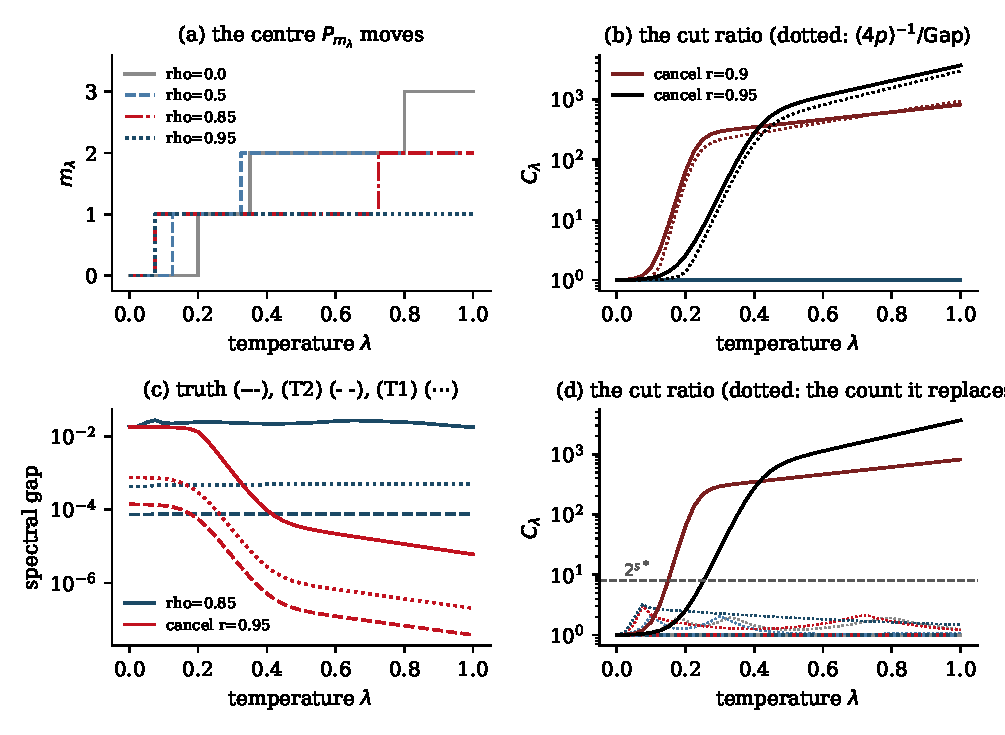
\includegraphics[width=\textwidth]{sec7_numerics.pdf}
        \caption{(a) the centre $P_{m_\lambda}$ of the ensemble as the
        temperature rises, for the four equicorrelated designs: it moves
        from $\emptyset$ to $\gamma^{\ast}$ in steps, one covariate at a
        time. (b) the cut ratio $C_\lambda$ of~\eqref{eq:cut}: it is $1$
        at every temperature on the four equicorrelated designs, and on the
        two cancelling designs it rises by three orders of magnitude,
        alongside the true deficit $(4p)^{-1}/\mathrm{Gap}(\mathbf{P}
        _\lambda)$ (dotted). (c) the exact gap, and the bounds
        \eqref{eq:gapfinal} and \eqref{eq:fibrebound}, for one design of each
        family. (d) the cut ratio $C_\lambda$ of~\eqref{eq:cut} (solid)
        against the precedent count
        $\max_z x_\lambda(z)/\bar\pi_\lambda(z)$ that \cref{rem:tie}
        discards (dotted), and its worst case $2^{s^{\ast}}$ (dashed).}
        \label{fig:sec7}
    \end{figure}

    \cref{tab:sec7} and \cref{fig:sec7} report the experiment. Five things
    are worth reading off.

    \begin{enumerate}[label=(\roman*),leftmargin=2.6em]
        \item \emph{The identity is an identity.} The largest deviation
        between $\lambda\log\mathcal{L}_n+\log\pi$ and $\log w_\lambda$, up
        to the additive constant, is $2.3\times10^{-13}$ --- machine
        precision, and the check that catches a wrong $\alpha$: with
        $\alpha$ taken as the nominal exponent $3/2$ of $g=p^{3}$ rather
        than as \eqref{eq:alphadef} defines it, the deviation is
        $7\times10^{-4}$.
        \item \emph{\cref{ass:BB} separates the two families, and
        \cref{prop:dip} is observed in both directions.} Clause
        \ref{B:exch} holds with zero slack on all six designs. Clause
        \ref{B:dim} holds on the four equicorrelated designs, with $3.9$ to
        $14.7$ nats to spare, and fails on both cancelling designs by
        $31.6$ and $49.9$ nats, the greedy gains there being
        $(-1.43,48.50)$ and $(-2.93,28.64)$: the second covariate is worth
        fifty nats once the first is in, and the first is worth nothing on
        its own. Correspondingly the ascent is uphill with $P_{m_\lambda}$
        its unique fixed point at all $41$ temperatures of each of the four,
        and at only $5$ and $8$ of the $41$ on the two.
        \item \emph{The cut ratio is the whole cost, and it tracks the
        truth.} $C_\lambda\leq1.008$ on the four equicorrelated designs, and
        $\varrho_\lambda=C_\lambda$ to five figures at every one of the
        $246$ pairs --- as~\eqref{eq:cutpairs} says it must, the bound being
        an identity. On the cancelling designs the exact gap really
        collapses, to $1.9\times10^{-5}$ and $6.0\times10^{-6}$ against
        $1/(4p)=1.8\times10^{-2}$, and $C_\lambda$ rises with it to $819$
        and $3671$ against true deficits $935$ and $2973$: it degrades where
        it must, and by the right amount, over three orders of magnitude.
        The precedent count that \cref{rem:tie} discards is $1.8$ to $3.2$
        times larger, and its worst case $2^{s^{\ast}}=8$ eight times larger
        again.
        \item \emph{The two flows are complementary, as \cref{rem:extremal}
        says, and both constants are sharp.} $M_\lambda$ agrees with the
        exact crossover congestion to within a factor $1.005$ to $1.023$ at
        every one of the $246$ pairs --- \eqref{eq:crossprop} is an
        inequality only because a single marginal is bounded by a coarser
        one --- and $C_\lambda$ is the ascent's congestion exactly. On these
        six designs the coordinates of $\gamma^{\ast}$ interact strongly, so
        the crossover is useless, its congestion reaching
        $1.6\times10^{1}$, $5.6\times10^{11}$, $2.0\times10^{26}$,
        $1.0\times10^{33}$ on the four equicorrelated designs, and the
        minimum in~\eqref{eq:gapfinal} is $C_\lambda$ at every pair. The roles
        reverse on the profile of \cref{rem:extremal}, where
        $C_\lambda=2^{s^{\ast}}/4$ and $M_\lambda=1$. The intermediate
        quantity $e^{2r_\lambda}$ of~\eqref{eq:crossprop}, which exists only
        to reach \cref{prop:pdefect}, is by contrast very loose here: with
        $r_\lambda$ up to $54.4$ nats it exceeds $M_\lambda$ by factors
        $7.6\times10^{3}$ to $5.9\times10^{18}$, and it should be read only
        as a near-product statement.
        \item \emph{The bound is valid and loses a fixed factor.} At all
        $246$ pairs both bounds hold. \eqref{eq:gapfinal} lies between
        $4.1\times10^{-3}$ and $8.9\times10^{-3}$ of the exact gap, a factor
        $112$ to $242$; \eqref{eq:fibrebound}, which differs only in the
        constants, between $2.4\times10^{-2}$ and $4.8\times10^{-2}$, a
        factor $21$ to $42$. Both hold uniformly in $\lambda$, including on
        the cancelling designs, where the truth itself has fallen by three
        orders of magnitude.
    \end{enumerate}

    \subsection{The gap as a function of $s^{\ast}$}
    \label{sub:sstar}

    \cref{rem:tie} claims that the exponential of the earlier estimate is a
    counting cost of the path method rather than a property of the chain,
    and that the cut ratio removes it. That is a testable claim, twice over:
    the truth should not decay in $s^{\ast}$, and neither should
    $C_\lambda$. We sweep the number of influential covariates, keeping
    everything else fixed.

    The truncation level is raised to $s_0=6$, so that $s^{\ast}$ may run to
    $5$, giving $\abs{\mathscr{M}(s_0)}=6476$ states; $n$, $p$, $\kappa$ and
    $g$ are as in \cref{sub:designs}. For each
    $\rho\in\{0,0.5,0.85,0.95\}$ and each $s^{\ast}\in\{1,\dots,5\}$ the
    influential columns are equicorrelated at $\rho$, the remaining ones are
    residualised against their span, and
    $\beta^{\ast}_S$ is the vector of the first $s^{\ast}$ entries of
    $(1.20,1.00,0.85,0.70,0.45)$ --- so that raising $s^{\ast}$ adds a
    covariate and changes nothing about the ones already there. Twenty-one
    temperatures are used, giving $420$ exactly computed gaps.

    \begin{table}[t]
        \centering
        \small
        \begin{tabular}{lrrrrrr}
            \hline
            $\rho$ & $s^{\ast}$ & \ref{B:exch} & \ref{B:dim}
            & $4p\min_\lambda\mathrm{Gap}$
            & $\max_\lambda C_\lambda$
            & $\min_\lambda\eqref{eq:gapfinal}$\\
            \hline
            $0$    & 1 & $0$ & --- & 1.000 & 1.00 & 2.8e-4\\
            $0$    & 2 & $0$ & $+19.1$ & 0.216 & 3.66 & 3.0e-5\\
            $0$    & 3 & $0$ & $+9.0$ & 0.210 & 4.05 & 1.5e-5\\
            $0$    & 4 & $0$ & $+11.0$ & 0.161 & 5.46 & 7.3e-6\\
            $0$    & 5 & $+0.025$ & $+7.2$ & 0.055 & 12.34 & 2.3e-6\\
            \hline
            $0.5$  & 5 & $+0.12$ & $-2.5$ & 0.999 & 1.90 & 1.5e-5\\
            $0.85$ & 4 & $+0.009$ & $-3.5$ & 0.584 & 1.77 & 2.3e-5\\
            $0.85$ & 5 & $+0.056$ & $-6.7$ & 0.787 & 1.49 & 1.9e-5\\
            $0.95$ & 5 & $0$ & $-1.4$ & 0.883 & 1.21 & 2.3e-5\\
            \hline
        \end{tabular}
        \caption{The $s^{\ast}$-sweep. The first block is the design
        $\rho=0$, the only one on which \ref{B:dim} fails; the second
        collects the rows of the other three designs at which anything
        happens at all --- at every row not shown,
        $4p\min_\lambda\mathrm{Gap}\in[0.899,1.006]$ and $C_\lambda\leq1.43$. Slacks are in nats, as in \cref{tab:sec7}; the
        entry \emph{---} is $s^{\ast}=1$, where \ref{B:dim} is vacuous. The
        full table is in \texttt{sec7\_sstar.txt}.}
        \label{tab:sstar}
    \end{table}

    \begin{figure}[t]
        \centering
        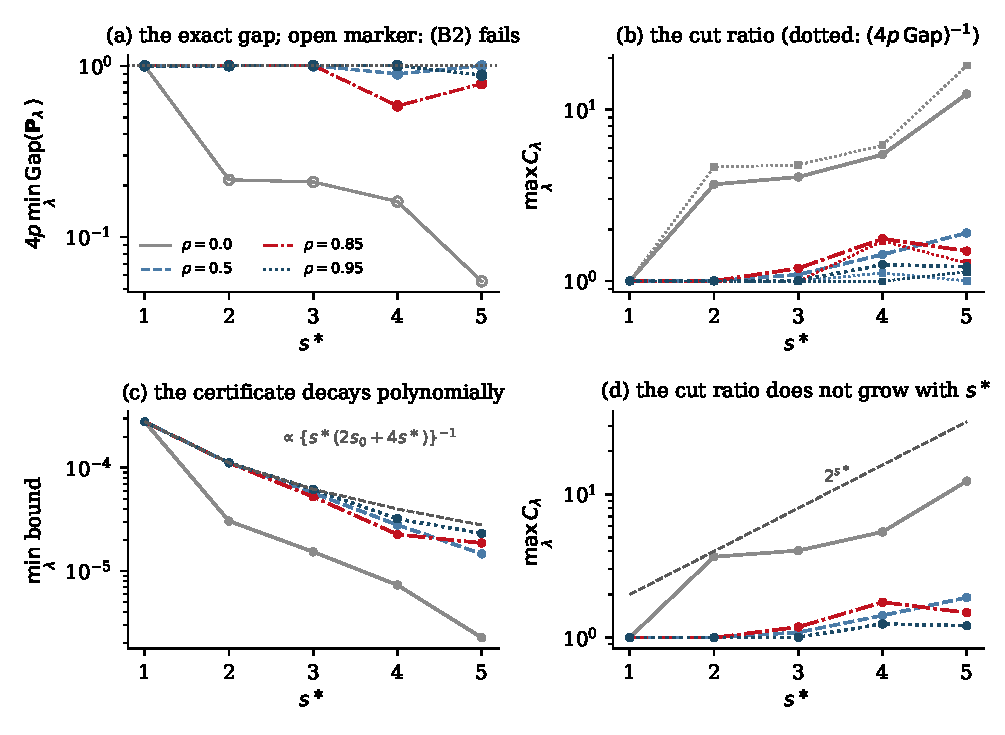
\includegraphics[width=\textwidth]{sec7_sstar.pdf}
        \caption{The gap as a function of $s^{\ast}$, at $s_0=6$. (a) the
        exact gap in units of $1/(4p)$, minimised over the temperature; an
        open marker means \ref{B:dim} fails. (b) the cut ratio
        $C_\lambda$ (solid) against the true deficit
        $\{4p\min_\lambda\mathrm{Gap}\}^{-1}$ (dotted, square markers).
        (c) the certificate \eqref{eq:gapfinal}, with a reference line
        $\propto\{s^{\ast}(2s_0+4s^{\ast})\}^{-1}$, the only way $s^{\ast}$
        enters \eqref{eq:gapfinal} once $C_\lambda$ is bounded. (d) the cut
        ratio $C_\lambda$ against $2^{s^{\ast}}$ (dashed), the worst case
        that \cref{rem:tie} removes.}
        \label{fig:sstar}
    \end{figure}

    \begin{enumerate}[label=(\roman*),leftmargin=2.6em]
        \item \emph{The number of influential covariates costs the chain
        nothing by itself.} At $\rho=0.5$ and $\rho=0.95$,
        $4p\min_\lambda\mathrm{Gap}(\mathbf{P}_\lambda)$ stays in
        $[0.883,1.006]$ for every $s^{\ast}$ from $1$ to $5$: the gap is
        $1/(4p)$, the rate of a single free coordinate, independently of how
        many influential covariates there are. Nothing in the truth resembles
        the $2^{s^{\ast}}$ that a precedent count would charge.
        \item \emph{Where the gap does decay in $s^{\ast}$, \ref{B:dim} is
        what fails, and $C_\lambda$ sees it.} The exception is $\rho=0$,
        where the profile $(1.20,1.00,\dots)$ is not geometric enough
        for~\eqref{eq:orth}: already at $s^{\ast}=2$ the greedy gains
        \emph{increase}, $g_0=18.37$ against $g_1=37.44$, \ref{B:dim} fails
        by $19.1$ nats, and the gap falls to $0.216/(4p)$, then to
        $0.055/(4p)$ at $s^{\ast}=5$. $C_\lambda$ follows: $3.66$, $4.05$,
        $5.46$, $12.34$ against true deficits $4.63$, $4.76$, $6.20$,
        $18.1$. So the $s^{\ast}$-dependence of the truth is a
        diminishing-returns effect and not a dimension effect. Note which
        way this runs: the worst design of the sweep is the
        \emph{orthogonal} one and the best are the correlated ones, because
        equicorrelation makes the first covariate account for most of the
        signal and the gains decay --- at $\rho=0.85$, $s^{\ast}=5$, they
        are $(82.1,24.0,12.9,3.4,-3.2)$ --- whereas at $\rho=0$ each
        covariate contributes on its own account and the gains can rise. No
        bound on $\nu$ or $\omega(X)$ distinguishes these designs the way
        \ref{B:dim} does.
        \item \emph{The cut ratio does not grow with $s^{\ast}$, and the
        certificate decays only polynomially.} Wherever \cref{ass:BB} holds,
        $C_\lambda$ is $1.00$, $1.00$, $1.01$--$1.19$, $1.25$--$1.77$,
        $1.21$--$1.90$ as $s^{\ast}$ runs from $1$ to $5$
        (\cref{fig:sstar}(d)): flat, and never as much as $2$. The
        certificate therefore falls only through the explicit factor
        $s^{\ast}(2s_0+4s^{\ast})$ of~\eqref{eq:gapfinal}, from
        $2.8\times10^{-4}$ to $1.5\times10^{-5}$, a factor $19$ over the
        sweep, tracking that reference line (\cref{fig:sstar}(c)). For
        comparison the precedent count that \cref{rem:tie} discards is the
        binomial count $\max_m\binom{s^{\ast}}m=1,2,3,6,10$, and the
        ensemble built on the greedy chain alone --- the one this
        construction replaced --- has exact congestion $1,2,3,6,10$ on the
        same rows and $3.9\times10^{2}$ at $\rho=0.5$, $s^{\ast}=5$. The
        exponential was in the route and in the estimate of it, and both are
        gone.
        \item \emph{\ref{B:exch} is the clause that gives way first, and the
        ascent absorbs it.} It holds exactly through $s^{\ast}=3$ on all
        four designs and begins to fail at $s^{\ast}=4$ on the collinear
        ones, by $0.009$ to $0.12$ nats. Because $F_\lambda$ takes the best
        admissible move rather than the prescribed one the damage is slight:
        at $\rho=0.5$, $s^{\ast}=5$, the ascent is uphill at $19$ of the
        $21$ temperatures and $C_\lambda=1.90$, against an exact gap of
        $0.999/(4p)$. The same row cost the greedy-chain ensemble a
        congestion of $3.9\times10^{2}$.
    \end{enumerate}

    All $420$ pairs satisfy both bounds of \cref{th:gapF}. Taking the two
    experiments together: the bound of \cref{th:gapF} is within a factor
    $640$ of the exact gap at every one of the $666$ (design, temperature)
    pairs computed in this section --- within $242$ at the $246$ pairs of
    \cref{sub:designs}, and within $640$ across the sweep, where $s_0$ is
    raised to $6$ --- it is uniform in $\lambda$, and its only non-explicit
    ingredient is a cut ratio that never exceeded $2$ wherever
    \cref{ass:BB} held.


    \begin{remark}[What the experiment does not test]
        \label{rem:regime}
        These are small designs, and none of the six of \cref{sub:designs}
        satisfies \cref{ass:betamin}, which asks
        $n\nu^{2}C_\beta^{2}/(\sigma_0^{2}\log p)\geq128(L+\Ltil+\alpha
        +\kappa)$, at least $832$ under \cref{ass:B,ass:C}: they deliver
        $2.7$, $1.1$, $0.11$, $0.014$, $5.3$ and $1.3$. The sweep is in the
        same position, and there the point needs no computation, since
        $\norm{X_j}_2^{2}=n$ forces $\nu\leq1$ and its designs deliver at
        most $nC_\beta^{2}/(\sigma_0^{2}\log p)=7.7$. At $p=14$ and $n=100$
        no design can do better, the requirement being asymptotic. What the
        experiment tests is therefore the construction and the quantities it
        carries, not the assumption set; \cref{sec:alltemp} in any case never
        uses \cref{ass:betamin}, which enters only through
        \cref{cor:critical,cor:half}, and the hypothesis it does use,
        \cref{ass:twosided}, holds on all six designs with the smallest
        admissible $a_0$ between $0.62$ and $0.88$ against the
        $\kappa+\alpha-2=1.50$ allowed.
    \end{remark}

    \bibliographystyle{imsart-nameyear}
    \bibliography{bvs}
    \appendix
    \section{Deferred proofs}
\label{sec:app}

% \begin{proof}[Proof of Lemma~\ref{lemma:master}]
%     Dividing numerator and denominator of the last fraction
%     in~\eqref{eq:Lik} by $g^{n/2}$, and writing $C_n(Y)$ for the
%     $\gamma$-free prefactor,
%     \begin{equation}
%         \label{eq:logL}
%         \log\mathcal{L}_n(Y\mid\gamma)
%         =\log C_n(Y)-\frac n2\log g
%         -\frac{\abs \gamma}{2}\log(1+g)
%         -\frac n2\log\bigl\{g^{-1}+1-R^{2}_\gamma\bigr\}.
%     \end{equation}
%     The first two terms of the right-hand side of~\eqref{eq:logL} do not
%     depend on $\gamma$, hence cancel in a difference:
%     \begin{equation}
%         \label{eq:logLratio}
%         \log\frac{\mathcal{L}_n(Y\mid\gamma)}
%         {\mathcal{L}_n(Y\mid\gamma')}
%         =\frac{\abs{\gamma'}-\abs \gamma}{2}\log(1+g)
%         +\frac n2\log\frac{g^{-1}+1-R^{2}_{\gamma'}}
%         {g^{-1}+1-R^{2}_{\gamma}} .
%     \end{equation}
%     By~\eqref{eq:prior} and~\eqref{eq:pilambda}, the normalising constants
%     cancelling,
%     \begin{equation*}
%         \log\frac{\pi_n^{(\lambda)}(\gamma\mid Y)}
%         {\pi_n^{(\lambda)}(\gamma'\mid Y)}
%         =\log\frac{\pi(\gamma)}{\pi(\gamma')}
%         +\lambda\log\frac{\mathcal{L}_n(Y\mid\gamma)}
%         {\mathcal{L}_n(Y\mid\gamma')}
%         =\kappa\bigl(\abs{\gamma'}-\abs \gamma\bigr)\log p
%         +\lambda\log\frac{\mathcal{L}_n(Y\mid\gamma)}
%         {\mathcal{L}_n(Y\mid\gamma')} .
%     \end{equation*}
%     Substituting~\eqref{eq:logLratio} and collecting the two terms
%     carrying the factor $\abs{\gamma'}-\abs \gamma$
%     gives~\eqref{eq:master}.
% \end{proof}

Every proof of the paper is collected here, together with the notation and
the deterministic bounds they rest on. Only the proof of \cref{th:drop}
involves the temperature, and it involves it only through the factor
$\lambda$ multiplying the fit term of~\eqref{eq:master}.

\subsection{Notation}
\label{sec:prelim}

We use throughout the effective noise of YWJ,
\begin{equation}
    \label{eq:wtilde}
    \widetilde w\ \coloneq\ X_{S^{c}}\beta^\ast_{S^{c}}+w,
    \qquad\text{so that}\qquad
    Y=\signal+\widetilde w ,
\end{equation}
the elementary inequalities
\begin{gather}
    \label{eq:elementary}
    \log(1+x)\leq x\ \ (x>-1),
    \qquad
    \norm{a+b}_2^{2}\leq2\norm a_2^{2}+2\norm b_2^{2},\\
    \nonumber
    \frac{a}{a+b}\geq\min\Bigl\{\frac12,\frac{a}{2b}\Bigr\}
    \ \ (a,b>0),
\end{gather}
and, for an underfitted $\gamma\in\mathscr{M}(s_0)$, the quantity
\begin{equation}
    \label{eq:Adef}
    A^{2}\ \coloneq\ \nu\,
    \frac{\norm{(I-\Phi_\gamma)\signal}_2^{2}}
    {\abs{\gamma^{\ast}\setminus\gamma}}\ >\ 0 ,
\end{equation}
the dependence on $\gamma$ being suppressed, as YWJ suppress it, since
$\gamma$ is fixed wherever $A$ occurs.


\subsection{Deterministic bounds}
\label{sub:appdet}

\begin{lemma}[Uniform residual lower bound]
    \label{lemma:residual}
    On the good event, and under~\eqref{eq:Dassumption}, every
    $\bar\gamma\in\mathscr{M}(s_0)$ satisfies
    \begin{equation}
        \label{eq:residual}
        \norm Y_2^{2}\bigl(g^{-1}+1-R^{2}_{\bar\gamma}\bigr)
        \ \geq\ \norm{(I-\Phi_{\bar\gamma})Y}_2^{2}
        \ \geq\ \frac{n\sigma_0^{2}}{8} .
    \end{equation}
\end{lemma}

\begin{proof}
    Since $\norm Y_2^{2}(g^{-1}+1-R^{2}_{\bar\gamma})
    =g^{-1}\norm Y_2^{2}+\norm{(I-\Phi_{\bar\gamma})Y}_2^{2}$, the first
    inequality amounts to discarding $g^{-1}\norm Y_2^{2}\geq0$. For the
    second, fix $\bar\gamma\in\mathscr{M}(s_0)$ and set
    $\bar\gamma^{+}\coloneq\bar\gamma\cup\gamma^{\ast}$, so that
    $\abs{\bar\gamma^{+}}\leq\abs{\bar\gamma}+s^{\ast}\leq s$ and
    $\bar\gamma^{+}\in\mathscr{M}(s)$. Since
    $\bar\gamma\subseteq\bar\gamma^{+}$, the range of $\Phi_{\bar\gamma}$
    is contained in that of $\Phi_{\bar\gamma^{+}}$, so
    $I-\Phi_{\bar\gamma}\succcurlyeq I-\Phi_{\bar\gamma^{+}}$ and
    \begin{equation}
        \label{eq:res1}
        \norm{(I-\Phi_{\bar\gamma})Y}_2^{2}
        \ \geq\ \norm{(I-\Phi_{\bar\gamma^{+}})Y}_2^{2}.
    \end{equation}
    Because $\gamma^{\ast}\subseteq\bar\gamma^{+}$, the vector $\signal$
    lies in the range of $\Phi_{\bar\gamma^{+}}$, so
    $(I-\Phi_{\bar\gamma^{+}})\signal=0$ and
    \begin{equation*}
    (I-\Phi_{\bar\gamma^{+}})
        Y
        =(I-\Phi_{\bar\gamma^{+}})w
        +(I-\Phi_{\bar\gamma^{+}})X_{S^{c}}\beta^\ast_{S^{c}} .
    \end{equation*}
    Apply $\norm{a+b}_2^{2}\geq\tfrac12\norm a_2^{2}-\norm b_2^{2}$, which
    is the rearrangement of $\tfrac12(\norm a_2-2\norm b_2)^{2}\geq0$,
    with $a=(I-\Phi_{\bar\gamma^{+}})w$ and
    $b=(I-\Phi_{\bar\gamma^{+}})X_{S^{c}}\beta^\ast_{S^{c}}$. Since
    projections are non-expansive, $\norm b_2^{2}\leq
    \norm{X_{S^{c}}\beta^\ast_{S^{c}}}_2^{2}\leq\Ltil\sigma_0^{2}\log p$
    by \cref{ass:A}, and $\norm a_2^{2}=\norm w_2^{2}
    -w^{\top}\Phi_{\bar\gamma^{+}}w$ because $I-\Phi_{\bar\gamma^+}$ is a
    projection. Hence
    \begin{equation*}
        \norm{(I-\Phi_{\bar\gamma^{+}})Y}_2^{2}
        \ \geq\ \tfrac12\bigl(\norm w_2^{2}
        -w^{\top}\Phi_{\bar\gamma^{+}}w\bigr)
        -\Ltil\sigma_0^{2}\log p .
    \end{equation*}
    On $\mathcal{C}_n$ we have $\norm w_2^{2}\geq n\sigma_0^{2}/2$, and on
    $\mathcal{B}_n$, applied to $\bar\gamma^{+}\in\mathscr{M}(s)$, we have
    $w^{\top}\Phi_{\bar\gamma^{+}}w\leq 8s\,\sigma_0^{2}\log p$.
    Therefore
    \begin{equation*}
        \norm{(I-\Phi_{\bar\gamma^{+}})Y}_2^{2}
        \ \geq\ \frac{n\sigma_0^{2}}{4}
        -\bigl\{4s+\Ltil\bigr\}\sigma_0^{2}\log p
        \ \geq\ \frac{n\sigma_0^{2}}{4}
        -\bigl\{8s+\Ltil\bigr\}\sigma_0^{2}\log p ,
    \end{equation*}
    and by~\eqref{eq:Dassumption} the subtracted term is at most
    $n\sigma_0^{2}/32$, so the right-hand side is at least
    $7n\sigma_0^{2}/32\geq n\sigma_0^{2}/8$. Combining
    with~\eqref{eq:res1} finishes the proof.
\end{proof}

\begin{lemma}[Effective noise]
    \label{lemma:noise}
    On the good event, and under~\eqref{eq:Dassumption}:
    \begin{equivcond}
        \item\label{it:noise_i}
        $\norm{\widetilde w}_2^{2}\leq2\Ltil\sigma_0^{2}\log p
        +3n\sigma_0^{2}$;
        \item\label{it:noise_ii} for every pair
        $\gamma_2\subset\gamma_1$ of $\mathscr{M}(s)$ with
        $\abs{\gamma_1}-\abs{\gamma_2}=1$,
        \begin{equation*}
            \norm{(\Phi_{\gamma_1}-\Phi_{\gamma_2})\widetilde w}_2^{2}
            \ \leq\ 2(L+\Ltil)\,\sigma_0^{2}\log p
            \ \leq\ \frac{n\nu^{2}C_\beta^{2}}{64} .
        \end{equation*}
    \end{equivcond}
\end{lemma}

\begin{proof}
    \ref{it:noise_i} By~\eqref{eq:elementary} and \cref{ass:A},
    $\norm{\widetilde w}_2^{2}\leq2\norm{X_{S^{c}}
        \beta^\ast_{S^{c}}}_2^{2}+2\norm w_2^{2}
    \leq2\Ltil\sigma_0^{2}\log p+2\norm w_2^{2}$, and on $\mathcal{C}_n$
    we have $\norm w_2^{2}\leq\tfrac32n\sigma_0^{2}$.

    \ref{it:noise_ii} Write $\Pi=\Phi_{\gamma_1}-\Phi_{\gamma_2}$, an
    orthogonal projection, so that $\norm{\Pi v}_2\leq\norm v_2$ for every
    $v$ and $\norm{\Pi w}_2^{2}=w^{\top}\Pi w$. Hence,
    by~\eqref{eq:elementary},
    \begin{align*}
        \norm{\Pi\widetilde w}_2^{2}
        &\leq2\norm{\Pi X_{S^{c}}\beta^\ast_{S^{c}}}_2^{2}
        +2\norm{\Pi w}_2^{2}
        \leq2\norm{X_{S^{c}}\beta^\ast_{S^{c}}}_2^{2}
        +2\,w^{\top}\bigl(\Phi_{\gamma_1}-\Phi_{\gamma_2}\bigr)w\\
        &\leq2\Ltil\sigma_0^{2}\log p+2L\sigma_0^{2}\log p,
    \end{align*}
    using \cref{ass:A} for the first term and the event $\mathcal{A}_n$,
    applied to the nested pair $\gamma_2\subset\gamma_1$ of
    $\mathscr{M}(s)$ with $\abs{\gamma_1}-\abs{\gamma_2}=1$, for the
    second. The final inequality is \cref{ass:betamin} rearranged, after
    discarding $\alpha+\kappa\geq0$ from its right-hand side; only the part
    $128(L+\Ltil)$ of that assumption is used here.
\end{proof}

\begin{lemma}[Upper bound on the regularised residual]
    \label{lemma:Dupper}
    On the good event, and under~\eqref{eq:Dassumption} and $n\geq3$, every
    $\gamma\in\mathscr{M}(s_0)$ satisfies
    \begin{equation}
        \label{eq:Dupper}
        \norm Y_2^{2}\bigl(g^{-1}+1-R^{2}_{\gamma}\bigr)
        \ \leq\ 2\norm{(I-\Phi_\gamma)\signal}_2^{2}
        +8\,n\sigma_0^{2} .
    \end{equation}
\end{lemma}

\begin{proof}
    By~\eqref{eq:wtilde} and~\eqref{eq:elementary},
    \begin{equation*}
        \norm{(I-\Phi_\gamma)Y}_2^{2}
        \leq2\norm{(I-\Phi_\gamma)\signal}_2^{2}
        +2\norm{(I-\Phi_\gamma)\widetilde w}_2^{2}
        \leq2\norm{(I-\Phi_\gamma)\signal}_2^{2}
        +2\norm{\widetilde w}_2^{2},
    \end{equation*}
    the last step because $I-\Phi_\gamma$ is a projection. By
    \cref{lemma:noise}\ref{it:noise_i}, $2\norm{\widetilde w}_2^{2}\leq
    4\Ltil\sigma_0^{2}\log p+6n\sigma_0^{2}$, and on $\mathcal{D}_n$ we
    have $g^{-1}\norm Y_2^{2}\leq(2\log p+3)\sigma_0^{2}$. Adding the two,
    the additive term is at most
    \begin{equation*}
        \bigl\{4\Ltil\log p+6n+2\log p+3\bigr\}\sigma_0^{2}
        \ \leq\ \Bigl\{\frac n8+6n+\frac{n}{128}+n\Bigr\}\sigma_0^{2}
        \ \leq\ 8n\sigma_0^{2},
    \end{equation*}
    where we used, in order: $\Ltil\log p\leq n/32$
    from~\eqref{eq:Dassumption}, whence $4\Ltil\log p\leq n/8$; the same display
    with $\Ltil$ replaced by $8s\geq8$, whence $\log p\leq n/256$ and
    $2\log p\leq n/128$; and $3\leq n$.
\end{proof}

\begin{lemma}[Greedy selection; YWJ, Lemma~8]
    \label{lemma:forward}
    Let $\gamma\in\mathscr{M}(s_0)$ be underfitted and let $j_\gamma$ be
    as in~\eqref{eq:jdef}. Under \cref{ass:B,ass:D,ass:betamin}:
    \begin{equivcond}
        \item\label{it:fs_a}
        $\norm{(\Phi_{\gamma\cup\{j_\gamma\}}-\Phi_\gamma)
            \signal}_2^{2}\geq A^{2}$, and moreover
        \begin{equation}
            \label{eq:Alower}
            A^{2}\ \geq\ n\,\nu^{2}\,
            \betabar{\gamma^{\ast}\setminus\gamma}
            \ \geq\ n\,\nu^{2}\min_{j\in\gamma^{\ast}}
            \abs{\beta^\ast_j}^{2}
            \ \geq\ n\,\nu^{2}C_\beta^{2} ;
        \end{equation}
        \item\label{it:fs_b} if in addition $\gamma$ is saturated and
        $k_\gamma$ is as in~\eqref{eq:kdef}, then, with
        $\widetilde\gamma=\gamma\cup\{j_\gamma\}$ and
        $\gamma'=\widetilde\gamma\setminus\{k_\gamma\}$,
        \begin{equation*}
            \norm{(\Phi_{\widetilde\gamma}-\Phi_{\gamma'})
                \signal}_2^{2}
            \ \leq\ n\,\omega(X)\,
            \frac{\norm{\beta^\ast_{\gamma^{\ast}\setminus\gamma}}_2^{2}}
            {s_0-s^{\ast}}
            \ \leq\ \frac{A^{2}}{4} .
        \end{equation*}
    \end{equivcond}
\end{lemma}

\begin{proof}
    We use two facts from YWJ. The first is their Lemma~7, the rank-one
    update formula: for $\bar\gamma\in\mathscr{M}(s)$ and
    $k\notin\bar\gamma$ with $\abs{\bar\gamma}<s$,
    \begin{equation}
        \label{eq:rankone}
        \Phi_{\bar\gamma\cup\{k\}}-\Phi_{\bar\gamma}
        =\frac{(I-\Phi_{\bar\gamma})X_kX_k^{\top}
            (I-\Phi_{\bar\gamma})}
        {X_k^{\top}(I-\Phi_{\bar\gamma})X_k},
    \end{equation}
    which follows from the block inversion formula applied to
    $X_{\bar\gamma\cup\{k\}}^{\top}X_{\bar\gamma\cup\{k\}}$. The second
    is their Lemma~6: under \cref{ass:B}, for every nested pair
    $\gamma_2\subset\gamma_1$ of $\mathscr{M}(s)$,
    \begin{equation}
        \label{eq:underfit}
        \lambda_{\min}\Bigl(\frac1n
        X_{\gamma_1\setminus\gamma_2}^{\top}
        (I-\Phi_{\gamma_2})X_{\gamma_1\setminus\gamma_2}\Bigr)
        \ \geq\ \nu ,
    \end{equation}
    because the matrix inside is $n$ times the Schur complement of the
    block $X_{\gamma_2}^{\top}X_{\gamma_2}$ in
    $X_{\gamma_1}^{\top}X_{\gamma_1}$, hence its inverse is the
    corresponding diagonal block of
    $(n^{-1}X_{\gamma_1}^{\top}X_{\gamma_1})^{-1}$, whose largest
    eigenvalue is at most
    $\lambda_{\min}(n^{-1}X_{\gamma_1}^{\top}X_{\gamma_1})^{-1}
    \leq\nu^{-1}$.

    \emph{Proof of~\ref{it:fs_a}.} Put $u\coloneq(I-\Phi_\gamma)\signal$.
    For $\ell\in\gamma^{\ast}\setminus\gamma$, idempotence of projections
    and~\eqref{eq:rankone} give
    \begin{align}
        \notag
        \norm{\Phi_{\gamma\cup\{\ell\}}\signal}_2^{2}
        -\norm{\Phi_{\gamma}\signal}_2^{2}
        &=(\beta^\ast_{\gamma^{\ast}})^{\top}
        X_{\gamma^{\ast}}^{\top}
        \bigl(\Phi_{\gamma\cup\{\ell\}}-\Phi_\gamma\bigr)\signal\\
        \label{eq:onegain}
        &=\frac{\langle X_\ell,u\rangle^{2}}
        {X_\ell^{\top}(I-\Phi_\gamma)X_\ell}
        \ \geq\ \frac{\langle X_\ell,u\rangle^{2}}{n},
    \end{align}
    where the last step uses
    $X_\ell^{\top}(I-\Phi_\gamma)X_\ell\leq\norm{X_\ell}_2^{2}=n$ and,
    for the middle equality, that
    $X_\ell^{\top}(I-\Phi_\gamma)\signal=\langle X_\ell,u\rangle$.
    Summing~\eqref{eq:onegain} over $\ell\in\gamma^{\ast}\setminus\gamma$,
    \begin{equation}
        \label{eq:sumgain}
        \sum_{\ell\in\gamma^{\ast}\setminus\gamma}
        \Bigl\{\norm{\Phi_{\gamma\cup\{\ell\}}\signal}_2^{2}
        -\norm{\Phi_{\gamma}\signal}_2^{2}\Bigr\}
        \ \geq\ \frac1n
        \norm{X_{\gamma^{\ast}\setminus\gamma}^{\top}u}_2^{2}
        \ =\ \frac1n\norm{X_{\gamma^{\ast}\cup\gamma}^{\top}u}_2^{2},
    \end{equation}
    the last equality because $X_j^{\top}u=0$ for $j\in\gamma$: indeed
    $X_j$ lies in the range of $\Phi_\gamma$, to which $u$ is orthogonal
    by construction. Now $u$ lies in the range of
    $X_{\gamma^{\ast}\cup\gamma}$, so $u=X_{\gamma^{\ast}\cup\gamma}v$ for
    some $v$; writing
    $M\coloneq X_{\gamma^{\ast}\cup\gamma}^{\top}
    X_{\gamma^{\ast}\cup\gamma}$, we have
    $\abs{\gamma^{\ast}\cup\gamma}\leq s$, hence $M\succcurlyeq n\nu I$ by
    \cref{ass:B}, and therefore
    \begin{equation*}
        \frac1n\norm{X_{\gamma^{\ast}\cup\gamma}^{\top}u}_2^{2}
        =\frac1nv^{\top}M^{2}v
        \ \geq\ \nu\,v^{\top}Mv
        =\nu\norm u_2^{2},
    \end{equation*}
    the inequality because $M^{2}-n\nu M=M^{1/2}(M-n\nu I)M^{1/2}
    \succcurlyeq0$. Combining with~\eqref{eq:sumgain} and dividing by
    $\abs{\gamma^{\ast}\setminus\gamma}$, the maximum over $\ell$ of the
    left-hand side of~\eqref{eq:onegain} is at least
    $\nu\norm u_2^{2}/\abs{\gamma^{\ast}\setminus\gamma}=A^{2}$. Since
    $j_\gamma$ attains that maximum by~\eqref{eq:jdef}, and since the
    left-hand side of~\eqref{eq:onegain} equals
    $\norm{(\Phi_{\gamma\cup\{\ell\}}-\Phi_\gamma)\signal}_2^{2}$ by
    idempotence, the first claim follows.

    For~\eqref{eq:Alower}, note that
    $(I-\Phi_\gamma)\signal=(I-\Phi_\gamma)
    X_{\gamma^{\ast}\setminus\gamma}
    \beta^\ast_{\gamma^{\ast}\setminus\gamma}$, because the columns $X_j$
    with $j\in\gamma^{\ast}\cap\gamma$ lie in the range of $\Phi_\gamma$;
    hence by~\eqref{eq:underfit} applied to
    $\gamma\subset\gamma^{\ast}\cup\gamma$,
    \begin{equation}
        \label{eq:usquare}
        \norm u_2^{2}
        =(\beta^\ast_{\gamma^{\ast}\setminus\gamma})^{\top}
        X_{\gamma^{\ast}\setminus\gamma}^{\top}(I-\Phi_\gamma)
        X_{\gamma^{\ast}\setminus\gamma}
        \beta^\ast_{\gamma^{\ast}\setminus\gamma}
        \ \geq\ n\,\nu
        \norm{\beta^\ast_{\gamma^{\ast}\setminus\gamma}}_2^{2},
    \end{equation}
    so that, using
    $\norm{\beta^\ast_{\gamma^{\ast}\setminus\gamma}}_2^{2}
    \geq\abs{\gamma^{\ast}\setminus\gamma}
    \min_{j\in\gamma^{\ast}}\abs{\beta^\ast_j}^{2}$ and~\eqref{eq:S},
    \begin{equation}
        \label{eq:Achain}
        A^{2}=\frac{\nu\norm u_2^{2}}
        {\abs{\gamma^{\ast}\setminus\gamma}}
        \ \geq\ \frac{n\nu^{2}
            \norm{\beta^\ast_{\gamma^{\ast}\setminus\gamma}}_2^{2}}
        {\abs{\gamma^{\ast}\setminus\gamma}}
        \ =\ n\nu^{2}\,\betabar{\gamma^{\ast}\setminus\gamma}
        \ \geq\ n\nu^{2}\min_{j\in\gamma^{\ast}}
        \abs{\beta^\ast_j}^{2}
        \ \geq\ n\nu^{2}C_\beta^{2} ,
    \end{equation}

    the middle equality being the definition~\eqref{eq:betabar} of the
    average. Only the last two inequalities are ever discarded, and
    \cref{sec:alltemp} keeps the average instead.

    \emph{Proof of~\ref{it:fs_b}.} Write
    $\widetilde\gamma=\gamma\cup\{j_\gamma\}$. For
    $\bar\gamma\in\mathscr{M}(s)$ let $\widehat\beta(\bar\gamma)$ solve
    \begin{equation}
        \label{eq:modLS}
        \min\bigl\{\norm{X\beta
        -X_{\gamma^{\ast}\setminus\widetilde\gamma}
            \beta^\ast_{\gamma^{\ast}\setminus\widetilde\gamma}}_2^{2}:\
        \beta\in\bbR^{p},\ \beta_j=0\ \text{for }j\notin\bar\gamma\bigr\},
    \end{equation}
    so that
    \begin{equation}
        \label{eq:LSid}
        \norm{X\widehat\beta(\bar\gamma)
        -X_{\gamma^{\ast}\setminus\widetilde\gamma}
            \beta^\ast_{\gamma^{\ast}\setminus\widetilde\gamma}}_2^{2}
        =\norm{(I-\Phi_{\bar\gamma})
            X_{\gamma^{\ast}\setminus\widetilde\gamma}
            \beta^\ast_{\gamma^{\ast}\setminus\widetilde\gamma}}_2^{2},
        \qquad
        \widehat\beta(\bar\gamma)_{\bar\gamma}
        =(X_{\bar\gamma}^{\top}X_{\bar\gamma})^{-1}X_{\bar\gamma}^{\top}
        X_{\gamma^{\ast}\setminus\widetilde\gamma}
        \beta^\ast_{\gamma^{\ast}\setminus\widetilde\gamma} .
    \end{equation}
    Since
    $k_\gamma\notin\gamma^\ast$ we have
    $\Phi_{\widetilde\gamma}X_{\gamma^{\ast}\cap\widetilde\gamma}
    =\Phi_{\widetilde\gamma\setminus\{k\}}
    X_{\gamma^{\ast}\cap\widetilde\gamma}$ for every
    $k\in\widetilde\gamma\setminus\gamma^{\ast}$, so with
    $\gamma'=\widetilde\gamma\setminus\{k_\gamma\}$
    \begin{align}
        \notag
        \norm{(\Phi_{\widetilde\gamma}-\Phi_{\gamma'})
            \signal}_2^{2}
        &=\norm{(\Phi_{\widetilde\gamma}-\Phi_{\gamma'})
            X_{\gamma^{\ast}\setminus\widetilde\gamma}
            \beta^\ast_{\gamma^{\ast}\setminus\widetilde\gamma}}_2^{2}\\
        \notag
        &=\norm{(I-\Phi_{\gamma'})
            X_{\gamma^{\ast}\setminus\widetilde\gamma}
            \beta^\ast_{\gamma^{\ast}\setminus\widetilde\gamma}}_2^{2}
        -\norm{(I-\Phi_{\widetilde\gamma})
            X_{\gamma^{\ast}\setminus\widetilde\gamma}
            \beta^\ast_{\gamma^{\ast}\setminus\widetilde\gamma}}_2^{2}\\
        \label{eq:LSdiff}
        &=\norm{X\widehat\beta(\gamma')
        -X_{\gamma^{\ast}\setminus\widetilde\gamma}
            \beta^\ast_{\gamma^{\ast}\setminus\widetilde\gamma}}_2^{2}
        -\norm{X\widehat\beta(\widetilde\gamma)
        -X_{\gamma^{\ast}\setminus\widetilde\gamma}
            \beta^\ast_{\gamma^{\ast}\setminus\widetilde\gamma}}_2^{2},
    \end{align}
    using in the second line that
    $\Phi_{\widetilde\gamma}-\Phi_{\gamma'}$ is a projection and
    $\gamma'\subset\widetilde\gamma$. By optimality of
    $\widehat\beta(\widetilde\gamma)$ in~\eqref{eq:modLS}, the residual
    $X\widehat\beta(\widetilde\gamma)
    -X_{\gamma^{\ast}\setminus\widetilde\gamma}
    \beta^\ast_{\gamma^{\ast}\setminus\widetilde\gamma}$ is orthogonal to
    $X_k$ for every $k\in\widetilde\gamma$, so for such $k$
    \begin{align*}
        \norm{X\widehat\beta(\widetilde\gamma\setminus\{k\})
        -X_{\gamma^{\ast}\setminus\widetilde\gamma}
            \beta^\ast_{\gamma^{\ast}\setminus\widetilde\gamma}}_2^{2}
        &\ \leq\ \norm{X\widehat\beta(\widetilde\gamma)
        -X_{\gamma^{\ast}\setminus\widetilde\gamma}
            \beta^\ast_{\gamma^{\ast}\setminus\widetilde\gamma}
            -X_k\widehat\beta_k(\widetilde\gamma)}_2^{2}\\
        &\ =\ \norm{X\widehat\beta(\widetilde\gamma)
        -X_{\gamma^{\ast}\setminus\widetilde\gamma}
            \beta^\ast_{\gamma^{\ast}\setminus\widetilde\gamma}}_2^{2}
        +\norm{X_k}_2^{2}\,
        \abs{\widehat\beta_k(\widetilde\gamma)}^{2},
    \end{align*}
    the first line because the vector $\widehat\beta(\widetilde\gamma)$
    with its $k$th coordinate zeroed is feasible for the problem defining
    $\widehat\beta(\widetilde\gamma\setminus\{k\})$, and the second by
    orthogonality. Since $\norm{X_k}_2^{2}=n$ and $k_\gamma$ minimises the
    left-hand side over $k\in\gamma\setminus\gamma^\ast
    =\widetilde\gamma\setminus(\gamma^{\ast}\cup\{j_\gamma\})$, whose
    cardinality is $s_0-\abs{\gamma\cap\gamma^{\ast}}\geq s_0-s^{\ast}$,
    \begin{equation*}
        \norm{X\widehat\beta(\gamma')
        -X_{\gamma^{\ast}\setminus\widetilde\gamma}
            \beta^\ast_{\gamma^{\ast}\setminus\widetilde\gamma}}_2^{2}
        -\norm{X\widehat\beta(\widetilde\gamma)
        -X_{\gamma^{\ast}\setminus\widetilde\gamma}
            \beta^\ast_{\gamma^{\ast}\setminus\widetilde\gamma}}_2^{2}
        \ \leq\ n\min_{k\in\gamma\setminus\gamma^\ast}
        \abs{\widehat\beta_k(\widetilde\gamma)}^{2}
        \ \leq\ \frac{n\norm{\widehat\beta(\widetilde\gamma)}_2^{2}}
        {s_0-s^{\ast}},
    \end{equation*}
    a minimum being at most the average. Finally
    \begin{equation*}
        \norm{\widehat\beta(\widetilde\gamma)}_2^{2}
        =\norm{(X_{\widetilde\gamma}^{\top}X_{\widetilde\gamma})^{-1}
            X_{\widetilde\gamma}^{\top}
            X_{\gamma^{\ast}\setminus\widetilde\gamma}
            \beta^\ast_{\gamma^{\ast}\setminus\widetilde\gamma}}_2^{2}
        \ \leq\ \omega(X)\,
        \norm{\beta^\ast_{\gamma^{\ast}
        \setminus\widetilde\gamma}}_2^{2}
        \ \leq\ \omega(X)\,
        \norm{\beta^\ast_{\gamma^{\ast}\setminus\gamma}}_2^{2},
    \end{equation*}
    by the definition of $\omega(X)$ in \cref{ass:D} and
    $\gamma^{\ast}\setminus\widetilde\gamma\subseteq
    \gamma^{\ast}\setminus\gamma$. Together with~\eqref{eq:LSdiff} this
    gives the first inequality of~\ref{it:fs_b}.

    For the second, combine
    $A^{2}\geq n\nu^{2}
    \norm{\beta^\ast_{\gamma^{\ast}\setminus\gamma}}_2^{2}/
    \abs{\gamma^{\ast}\setminus\gamma}\geq
    n\nu^{2}\norm{\beta^\ast_{\gamma^{\ast}\setminus\gamma}}_2^{2}/
    s^{\ast}$, which is~\eqref{eq:Achain}, with the first inequality of
    \cref{ass:D}: $s_0\geq(4\nu^{-2}\omega(X)+1)s^{\ast}$ is equivalent to
    $4\omega(X)s^{\ast}\leq\nu^{2}(s_0-s^{\ast})$, that is to
    \begin{equation*}
        \frac{n\,\omega(X)
        \norm{\beta^\ast_{\gamma^{\ast}\setminus\gamma}}_2^{2}}
        {s_0-s^{\ast}}
        \ \leq\ \frac14\cdot
        \frac{n\,\nu^{2}
            \norm{\beta^\ast_{\gamma^{\ast}\setminus\gamma}}_2^{2}}
        {s^{\ast}}
        \ \leq\ \frac{A^{2}}{4} . \qedhere
    \end{equation*}
\end{proof}


\begin{remark}
    \label{rem:ywj_constant}
    With their constant $2$ in place of our $4$ in~\eqref{eq:Dassumption},
    YWJ obtain $\norm{v_2}_2\leq A/\sqrt2$ rather than
    $\norm{v_2}_2\leq A/2$, and combine it with a noise bound $A/4$. The
    resulting numbers do not close: on their page~2527 the displayed lower
    bound $A(A-A/4)-(A/\sqrt2)(A/\sqrt2+A/4)-A^{2}/16$ equals
    $0.0107\,A^{2}$, not the $A^{2}/8$ claimed, and it is negative if one
    keeps the factor $2$ that their own preceding display carries on the
    cross terms. Strengthening \cref{ass:D} to
    $s_0\geq(4\nu^{-2}\omega(X)+1)s^{\ast}$, and \cref{ass:betamin} so
    that the noise budget is $A/8$ rather than $A/4$, repairs this with
    room to spare; see~\eqref{eq:satdrop} below. Nothing else in their
    argument, or in ours, is affected.
\end{remark}

\begin{lemma}[Proxy bound]
    \label{lemma:proxy}
    For every $\gamma\in\mathscr{M}(s)$ and every
    $j\in\gamma\setminus\gamma^{\ast}$,
    \begin{equation}
        \label{eq:proxy}
        \bigl\|(\Phi_{\gamma}-\Phi_{\gamma\setminus\{j\}})
        \signal\bigr\|_2^{2}
        \ \leq\ n\,\omega(X)\,
        \bigl\|\beta^{\ast}_{\gamma^{\ast}\setminus\gamma}\bigr\|_2^{2} .
    \end{equation}
\end{lemma}

\begin{proof}
    This is the chain of displays in the proof of
    \cref{lemma:forward}\ref{it:fs_b}, run with $\widetilde\gamma$
    replaced by $\gamma$ and $k_\gamma$ by $j$. Every step used only
    $j\notin\gamma^{\ast}$ and $\gamma\in\mathscr{M}(s)$: first
    $\Phi_{\gamma}X_{\gamma^{\ast}\cap\gamma}
    =\Phi_{\gamma\setminus\{j\}}X_{\gamma^{\ast}\cap\gamma}$, so the left
    side equals $\|(\Phi_\gamma-\Phi_{\gamma\setminus\{j\}})
    X_{\gamma^{\ast}\setminus\gamma}
    \beta^{\ast}_{\gamma^{\ast}\setminus\gamma}\|_2^{2}$; then the
    identification with a difference of least-squares residuals; then
    feasibility of zeroing the $j$th coordinate, which gives the bound
    $n\abs{\widehat\beta_j(\gamma)}^{2}$; then
    $\|\widehat\beta(\gamma)\|_2^{2}\leq\omega(X)
    \|\beta^{\ast}_{\gamma^{\ast}\setminus\gamma}\|_2^{2}$. Taking
    $\gamma\supseteq\gamma^{\ast}$ makes the right side vanish and
    recovers the identity used in \cref{sub:over}.
\end{proof}

\subsection{Counting and paths}
\label{sub:appcount}

\begin{lemma}[Counting precedents]
    \label{lemma:count}
    Let $\bar\eta\in\mathscr{M}(s_0)$.
    \begin{equivcond}
        \item\label{it:cnt_i} $\mathcal{G}$ maps overfitted states to
        states containing $\gamma^{\ast}$. Consequently, if $\gamma$ is
        underfitted then every $\bar\gamma\in\Lambda(\gamma)$ is
        underfitted.
        \item\label{it:cnt_ii} $\bar\eta$ has at most $(s^{\ast}+1)p$
        immediate precedents that are underfitted --- that is, states
        $\bar\gamma\neq\bar\eta$ with
        $\mathcal{G}(\bar\gamma)=\bar\eta$ and $\bar\gamma$ underfitted
        --- and at most $p$ that are overfitted.
        \item\label{it:cnt_iii} Hence, for every $k\geq0$, the number of
        $\bar\gamma$ with $\mathcal{G}^{k}(\bar\gamma)=\bar\eta$ and
        $\bar\gamma,\mathcal{G}(\bar\gamma),\dots,
        \mathcal{G}^{k-1}(\bar\gamma)$ all underfitted is at most
        $\{(s^{\ast}+1)p\}^{k}$; and if
        $\bar\eta\supseteq\gamma^{\ast}$, the number of overfitted
        $\bar\gamma\in\Lambda_k(\bar\eta)$ is at most $p^{k}$.
    \end{equivcond}
\end{lemma}

\begin{proof}
    \ref{it:cnt_i} An overfitted $\bar\gamma$ is treated by
    rule~\ref{G:del}, which deletes
    $\ell_{\bar\gamma}\in\bar\gamma\setminus\gamma^{\ast}$ and therefore
    leaves $\gamma^{\ast}\subseteq\mathcal{G}(\bar\gamma)$; and
    $\gamma^{\ast}$ is a fixed point. So
    $\mathcal{G}^{k}(\bar\gamma)\supseteq\gamma^{\ast}$ for every
    $k\geq0$, and no such state is underfitted.

    \ref{it:cnt_ii} Let $\bar\gamma\neq\bar\eta$ be underfitted with
    $\mathcal{G}(\bar\gamma)=\bar\eta$. If rule~\ref{G:add} applies then
    $\bar\eta=\bar\gamma\cup\{j_{\bar\gamma}\}$ with
    $j_{\bar\gamma}\in\gamma^{\ast}$, so
    $\bar\gamma=\bar\eta\setminus\{j\}$ for some
    $j\in\gamma^{\ast}\cap\bar\eta$: at most $s^{\ast}$ states. If
    rule~\ref{G:exch} applies then
    $\bar\eta=\bar\gamma\cup\{j_{\bar\gamma}\}
    \setminus\{k_{\bar\gamma}\}$ with $j_{\bar\gamma}\in\gamma^{\ast}$
    and $k_{\bar\gamma}\in S^{c}$, so
    $\bar\gamma=\bar\eta\cup\{k\}\setminus\{j\}$ with
    $j\in\gamma^{\ast}\cap\bar\eta$ and $k\in S^{c}$: at most
    $s^{\ast}(p-s^{\ast})$ states. The total is at most
    $s^{\ast}(1+p-s^{\ast})\leq s^{\ast}(1+p)\leq(s^{\ast}+1)p$, the last
    step because $s^{\ast}\leq p$. If instead $\bar\gamma$ is overfitted
    then rule~\ref{G:del} applies and $\bar\gamma=\bar\eta\cup\{\ell\}$
    with $\ell\in S^{c}$: at most $p$ states.

    \ref{it:cnt_iii} Iterate~\ref{it:cnt_ii}: a state counted at level
    $k$ is an immediate precedent, of the stated type, of one counted at
    level $k-1$. For the second claim, \ref{it:cnt_i} shows that an
    overfitted $\bar\gamma\in\Lambda_k(\bar\eta)$ reaches $\bar\eta$
    through states containing $\gamma^{\ast}$ only, so each of the $k$
    steps deletes an index of $S^{c}$; hence
    $\bar\gamma=\bar\eta\cup u$ with $u\subseteq S^{c}$ and $\abs u=k$,
    and there are at most $\binom{p}{k}\leq p^{k}$ such $u$.
\end{proof}

\begin{lemma}[Path properties; YWJ, Lemma~2]
    \label{lemma:paths}
    \begin{equivcond}
        \item\label{it:pp_i} $\mathcal{G}^{k}(\gamma)=\gamma^{\ast}$ for
        some $k\leq d_H(\gamma,\gamma^{\ast})$, every
        $\gamma\in\mathscr{M}(s_0)$; in particular
        $\Lambda(\gamma^{\ast})=\mathscr{M}(s_0)$.
        \item\label{it:pp_ii} $\abs{T_{\gamma,\gamma^{\ast}}}\leq
        d_H(\gamma,\gamma^{\ast})\leq s_0+s^{\ast}\leq2s_0$, and
        $\ell(\mathcal{T})\leq4s_0$.
        \item\label{it:pp_iii} For a directed edge
        $e=(\bar\gamma,\mathcal{G}(\bar\gamma))$,
        \begin{equation*}
            \bigl\{(\gamma,\gamma'):T_{\gamma,\gamma'}\ni e\bigr\}
            \ \subseteq\ \Lambda(\bar\gamma)\times\mathscr{M}(s_0) .
        \end{equation*}
    \end{equivcond}
\end{lemma}

\begin{proof}
    \ref{it:pp_i} By the second remark after \cref{def:G},
    $d_H(\mathcal{G}(\gamma),\gamma^{\ast})<d_H(\gamma,\gamma^{\ast})$
    whenever $\gamma\neq\gamma^{\ast}$, so the orbit reaches the unique
    fixed point $\gamma^{\ast}$ in at most
    $d_H(\gamma,\gamma^{\ast})$ steps. Hence every state lies in
    $\Lambda(\gamma^{\ast})$.

    \ref{it:pp_ii} Each step of $\mathcal{G}$ decreases
    $d_H(\cdot,\gamma^{\ast})$ by at least one, so the orbit has at most
    $d_H(\gamma,\gamma^{\ast})$ edges; and
    $d_H(\gamma,\gamma^{\ast})\leq\abs\gamma+\abs{\gamma^{\ast}}
    \leq s_0+s^{\ast}$, which is at most $2s_0$ because
    $s^{\ast}<s_0$. Since $T_{\gamma,\gamma'}$ is contained in the
    concatenation of $T_{\gamma,\gamma^{\ast}}$ with the reverse of
    $T_{\gamma',\gamma^{\ast}}$, its length is at most $4s_0$.

    \ref{it:pp_iii} By construction $T_{\gamma,\gamma'}$ traverses its
    first segment in the direction of $\mathcal{G}$ and its second
    segment against it. The edge $e$ points in the direction of
    $\mathcal{G}$, so it can only occur in the first segment, which is
    part of $T_{\gamma,\gamma^{\ast}}$. Hence $\bar\gamma\in
    T_{\gamma,\gamma^{\ast}}$, that is $\gamma\in\Lambda(\bar\gamma)$,
    while $\gamma'$ is unconstrained.
\end{proof}

\subsection{Proof of \cref{th:drop}: overfitted states}
\label{sub:over}

Throughout \cref{sub:over,sub:under,sub:sat} we write
$\gamma'\coloneq\mathcal{G}(\gamma)$ and start from~\eqref{eq:master} with
the size change read off from~\eqref{eq:sizechange}.

Here $\gamma\supseteq\gamma^{\ast}$, $\gamma\neq\gamma^{\ast}$, and
rule~\ref{G:del} applies: $\gamma'=\gamma\setminus\{\ell_\gamma\}$ with
$\ell_\gamma\in\gamma\setminus\gamma^\ast$, so
$\abs{\gamma'}-\abs \gamma=-1$ and \eqref{eq:master} gives
\begin{equation}
    \label{eq:over1}
    \log\frac{\pi_n^{(\lambda)}(\gamma\mid Y)}
    {\pi_n^{(\lambda)}(\gamma'\mid Y)}
    \ =\ -\kappa\log p-\lambda\alpha\log p
    +\frac{\lambda n}{2}
    \log\frac{g^{-1}+1-R^{2}_{\gamma'}}{g^{-1}+1-R^{2}_{\gamma}} .
\end{equation}
Since $\gamma'\subset\gamma$ and $\abs \gamma-\abs{\gamma'}=1$, the matrix
$\Phi_\gamma-\Phi_{\gamma'}$ is an orthogonal projection of rank one, and
\begin{equation}
    \label{eq:over1b}
    \norm Y_2^{2}\bigl(R^{2}_{\gamma}-R^{2}_{\gamma'}\bigr)
    =Y^{\top}(\Phi_\gamma-\Phi_{\gamma'})Y
    =\norm{(\Phi_\gamma-\Phi_{\gamma'})Y}_2^{2}\ \geq\ 0 ,
\end{equation}
so that, using $\log(1+x)\leq x$ and then \cref{lemma:residual},
\begin{equation}
    \label{eq:over2}
    \frac n2\log\frac{g^{-1}+1-R^{2}_{\gamma'}}
    {g^{-1}+1-R^{2}_{\gamma}}
    =\frac n2\log\Bigl(1+\frac{\norm{(\Phi_\gamma-\Phi_{\gamma'})
        Y}_2^{2}}{\norm Y_2^{2}(g^{-1}+1-R^{2}_{\gamma})}\Bigr)
    \ \leq\ \frac n2\cdot
    \frac{8\norm{(\Phi_\gamma-\Phi_{\gamma'})Y}_2^{2}}{n\sigma_0^{2}} .
\end{equation}
It remains to bound $\norm{(\Phi_\gamma-\Phi_{\gamma'})Y}_2^{2}$. Since
$\ell_\gamma\notin\gamma^\ast$ and $\gamma^{\ast}\subseteq\gamma$, we have
$\gamma^{\ast}\subseteq\gamma'$, so $\signal$ lies in the range of
$\Phi_{\gamma'}$; and $\Phi_\gamma-\Phi_{\gamma'}$ annihilates that range,
because for $v$ in it $\Phi_\gamma v=v$, the range of $\Phi_{\gamma'}$
being contained in that of $\Phi_\gamma$, so that
$(\Phi_\gamma-\Phi_{\gamma'})v=v-v=0$. Hence, by~\eqref{eq:wtilde},
\begin{equation}
    \label{eq:over3}
    (\Phi_\gamma-\Phi_{\gamma'})Y
    =(\Phi_\gamma-\Phi_{\gamma'})\widetilde w,
    \qquad\text{so}\qquad
    \norm{(\Phi_\gamma-\Phi_{\gamma'})Y}_2^{2}
    \ \leq\ 2(L+\Ltil)\sigma_0^{2}\log p
\end{equation}
by \cref{lemma:noise}\ref{it:noise_ii}, applied to the nested pair
$\gamma'\subset\gamma$ of
$\mathscr{M}(s_0)\subseteq\mathscr{M}(s)$ with
$\abs \gamma-\abs{\gamma'}=1$. Substituting~\eqref{eq:over3}
into~\eqref{eq:over2},
\begin{equation}
    \label{eq:over4}
    \frac n2\log\frac{g^{-1}+1-R^{2}_{\gamma'}}
    {g^{-1}+1-R^{2}_{\gamma}}\ \leq\ 8(L+\Ltil)\log p ,
\end{equation}
and substituting this into~\eqref{eq:over1}, using $\lambda\geq0$ so that
multiplying~\eqref{eq:over4} by $\lambda$ preserves the inequality,
\begin{equation*}
    \log\frac{\pi_n^{(\lambda)}(\gamma\mid Y)}
    {\pi_n^{(\lambda)}(\gamma'\mid Y)}
    \ \leq\ -\kappa\log p
    -\lambda\bigl\{\alpha-8(L+\Ltil)\bigr\}\log p ,
\end{equation*}
which is~\eqref{eq:drop_over}. \qed

\subsection{Proof of \cref{th:drop}: underfitted, unsaturated states}
\label{sub:under}

Here $\gamma^{\ast}\setminus\gamma\neq\emptyset$ and $\abs \gamma<s_0$, so
rule~\ref{G:add} applies: $\gamma'=\gamma\cup\{j_\gamma\}$,
$\abs{\gamma'}-\abs \gamma=+1$, and \eqref{eq:master} gives
\begin{equation}
    \label{eq:und1}
    \log\frac{\pi_n^{(\lambda)}(\gamma\mid Y)}
    {\pi_n^{(\lambda)}(\gamma'\mid Y)}
    \ =\ \kappa\log p+\lambda\alpha\log p
    +\frac{\lambda n}{2}
    \log\frac{g^{-1}+1-R^{2}_{\gamma'}}{g^{-1}+1-R^{2}_{\gamma}} .
\end{equation}
Note $s^{\ast}\geq1$, since $\gamma^{\ast}\setminus\gamma\neq\emptyset$.
The matrix $\Phi_{\gamma'}-\Phi_\gamma$ is an orthogonal projection of
rank one, and as in~\eqref{eq:over1b},
\begin{equation}
    \label{eq:und1b}
    \norm Y_2^{2}\bigl(R^{2}_{\gamma'}-R^{2}_{\gamma}\bigr)
    =\norm{(\Phi_{\gamma'}-\Phi_{\gamma})Y}_2^{2} ,
\end{equation}
so that, by $\log(1+x)\leq x$ applied with
$x=-\norm{(\Phi_{\gamma'}-\Phi_\gamma)Y}_2^{2}/
\{\norm Y_2^{2}(g^{-1}+1-R^{2}_\gamma)\}\in(-1,0]$,
\begin{equation}
    \label{eq:und2}
    \frac n2\log\frac{g^{-1}+1-R^{2}_{\gamma'}}
    {g^{-1}+1-R^{2}_{\gamma}}
    \ \leq\ -\frac n2\cdot
    \frac{\norm{(\Phi_{\gamma'}-\Phi_\gamma)Y}_2^{2}}
    {\norm Y_2^{2}\bigl(g^{-1}+1-R^{2}_{\gamma}\bigr)} .
\end{equation}

\emph{Step 1: the numerator.} By \cref{lemma:forward}\ref{it:fs_a},
$\norm{(\Phi_{\gamma'}-\Phi_\gamma)\signal}_2\geq A$, and by
\cref{lemma:noise}\ref{it:noise_ii} applied to the nested pair
$\gamma\subset\gamma'$, together with~\eqref{eq:Alower},
\begin{equation}
    \label{eq:und3}
    \norm{(\Phi_{\gamma'}-\Phi_\gamma)\widetilde w}_2^{2}
    \ \leq\ \frac{n\nu^{2}C_\beta^{2}}{64}\ \leq\ \frac{A^{2}}{64},
    \qquad\text{that is}\qquad
    \norm{(\Phi_{\gamma'}-\Phi_\gamma)\widetilde w}_2
    \leq\frac{A}{8} .
\end{equation}
Hence, by the triangle inequality and~\eqref{eq:wtilde},
\begin{equation}
    \label{eq:und4}
    \norm{(\Phi_{\gamma'}-\Phi_\gamma)Y}_2
    \ \geq\ A-\frac{A}{8}=\frac{7A}{8}\ >\ 0,
    \quad\text{so}\quad
    \norm{(\Phi_{\gamma'}-\Phi_\gamma)Y}_2^{2}
    \ \geq\ \tfrac{49}{64}A^{2}\ \geq\ \tfrac12A^{2} .
\end{equation}

\emph{Step 2: the denominator.} By \cref{lemma:Dupper} and the
definition~\eqref{eq:Adef}, which gives
$\norm{(I-\Phi_\gamma)\signal}_2^{2}
=\abs{\gamma^{\ast}\setminus\gamma}A^{2}/\nu\leq s^{\ast}A^{2}/\nu$,
\begin{equation}
    \label{eq:und5}
    \norm Y_2^{2}\bigl(g^{-1}+1-R^{2}_{\gamma}\bigr)
    \ \leq\ \frac{2s^{\ast}A^{2}}{\nu}+8n\sigma_0^{2} .
\end{equation}

\emph{Step 3: combining.} By~\eqref{eq:und4} and~\eqref{eq:und5}, then by
the third inequality of~\eqref{eq:elementary} with
$a=2s^{\ast}A^{2}/\nu>0$ and $b=8n\sigma_0^{2}>0$,
\begin{equation}
    \label{eq:und6}
    \frac n2\cdot
    \frac{\norm{(\Phi_{\gamma'}-\Phi_\gamma)Y}_2^{2}}
    {\norm Y_2^{2}(g^{-1}+1-R^{2}_{\gamma})}
    \ \geq\ \frac n4\cdot\frac{A^{2}}
    {2s^{\ast}A^{2}/\nu+8n\sigma_0^{2}}
    \ =\ \frac{n\nu}{8s^{\ast}}\cdot\frac{a}{a+b}
    \ \geq\ \frac{n\nu}{8s^{\ast}}
    \min\Bigl\{\frac12,\frac{s^{\ast}A^{2}}
    {8\nu n\sigma_0^{2}}\Bigr\} ,
\end{equation}
that is, distributing $n\nu/(8s^{\ast})$ over the minimum and then
using $A^{2}\geq n\nu^{2}C_\beta^{2}$ from~\eqref{eq:Alower},
\begin{equation}
    \label{eq:und8}
    \frac n2\cdot
    \frac{\norm{(\Phi_{\gamma'}-\Phi_\gamma)Y}_2^{2}}
    {\norm Y_2^{2}(g^{-1}+1-R^{2}_{\gamma})}
    \ \geq\ \min\Bigl\{\frac{n\nu}{16s^{\ast}},\
    \frac{A^{2}}{64\,\sigma_0^{2}}\Bigr\}
    \ \geq\ \gainfloor .
\end{equation}
Combining \eqref{eq:und1}, \eqref{eq:und2} and~\eqref{eq:und8}, and using
$\lambda\geq0$,
\begin{equation*}
    \log\frac{\pi_n^{(\lambda)}(\gamma\mid Y)}
    {\pi_n^{(\lambda)}(\gamma'\mid Y)}
    \ \leq\ \kappa\log p
    +\lambda\Bigl\{\alpha\log p-\gainfloor\Bigr\} ,
\end{equation*}
which is~\eqref{eq:drop_unsat}. \qed

\subsection{Proof of \cref{th:drop}: underfitted, saturated states}
\label{sub:sat}

Here $\gamma^{\ast}\setminus\gamma\neq\emptyset$ and $\abs \gamma=s_0$, so
rule~\ref{G:exch} applies: with
$\widetilde\gamma=\gamma\cup\{j_\gamma\}$ and
$\gamma'=\widetilde\gamma\setminus\{k_\gamma\}$ we have
$\abs{\gamma'}=\abs \gamma$, and \eqref{eq:master} gives
\begin{equation}
    \label{eq:sat1}
    \log\frac{\pi_n^{(\lambda)}(\gamma\mid Y)}
    {\pi_n^{(\lambda)}(\gamma'\mid Y)}
    \ =\ \frac{\lambda n}{2}
    \log\frac{g^{-1}+1-R^{2}_{\gamma'}}{g^{-1}+1-R^{2}_{\gamma}} ,
\end{equation}
the inclusion penalty having cancelled identically. Note that
$\widetilde\gamma\in\mathscr{M}(s)$, since
$\abs{\widetilde\gamma}=s_0+1\leq s$, and that both $\gamma$ and $\gamma'$
are subsets of $\widetilde\gamma$ of cardinality
$\abs{\widetilde\gamma}-1$, so that
$\Phi_{\widetilde\gamma}-\Phi_\gamma$ and
$\Phi_{\widetilde\gamma}-\Phi_{\gamma'}$ are orthogonal projections of
rank one. Following YWJ, set
\begin{equation}
    \label{eq:vdef}
    v_1\coloneq(\Phi_{\widetilde\gamma}-\Phi_\gamma)\signal,
    \qquad
    v_2\coloneq(\Phi_{\widetilde\gamma}-\Phi_{\gamma'})\signal .
\end{equation}
Adding and subtracting $Y^{\top}\Phi_{\widetilde\gamma}Y$,
\begin{equation}
    \label{eq:sat2}
    \norm Y_2^{2}\bigl(R^{2}_{\gamma'}-R^{2}_{\gamma}\bigr)
    =Y^{\top}\Phi_{\gamma'}Y-Y^{\top}\Phi_{\gamma}Y
    =\norm{(\Phi_{\widetilde\gamma}-\Phi_\gamma)Y}_2^{2}
    -\norm{(\Phi_{\widetilde\gamma}-\Phi_{\gamma'})Y}_2^{2} .
\end{equation}
By \cref{lemma:forward}\ref{it:fs_a} and~\ref{it:fs_b},
$\norm{v_1}_2\geq A$ and $\norm{v_2}_2\leq A/2$; and by
\cref{lemma:noise}\ref{it:noise_ii} applied to each of the two nested
pairs $\gamma\subset\widetilde\gamma$ and
$\gamma'\subset\widetilde\gamma$ of $\mathscr{M}(s)$, exactly as
in~\eqref{eq:und3},
\begin{equation}
    \label{eq:sat4}
    \norm{(\Phi_{\widetilde\gamma}-\Phi_\gamma)\widetilde w}_2
    \ \leq\ \frac{A}{8},
    \qquad
    \norm{(\Phi_{\widetilde\gamma}-\Phi_{\gamma'})\widetilde w}_2
    \ \leq\ \frac{A}{8} .
\end{equation}
Therefore, by the triangle inequality applied to
$(\Phi_{\widetilde\gamma}-\Phi_\gamma)Y=v_1
+(\Phi_{\widetilde\gamma}-\Phi_\gamma)\widetilde w$ and to
$(\Phi_{\widetilde\gamma}-\Phi_{\gamma'})Y=v_2
+(\Phi_{\widetilde\gamma}-\Phi_{\gamma'})\widetilde w$,
\begin{equation}
    \label{eq:sat5}
    \norm{(\Phi_{\widetilde\gamma}-\Phi_\gamma)Y}_2
    \ \geq\ A-\frac{A}{8}=\frac{7A}{8}\ >\ 0,
    \qquad
    \norm{(\Phi_{\widetilde\gamma}-\Phi_{\gamma'})Y}_2
    \ \leq\ \frac{A}{2}+\frac{A}{8}=\frac{5A}{8} ,
\end{equation}
and squaring, which is legitimate because both bounds are non-negative,
\begin{equation}
    \label{eq:satdrop}
    \norm Y_2^{2}\bigl(R^{2}_{\gamma'}-R^{2}_{\gamma}\bigr)
    \ \geq\ \frac{49}{64}A^{2}-\frac{25}{64}A^{2}
    \ =\ \frac{24}{64}A^{2}\ \geq\ \frac{A^{2}}{4}\ >\ 0 .
\end{equation}
Inequality~\eqref{eq:und2} holds verbatim, with
$\norm{(\Phi_{\gamma'}-\Phi_\gamma)Y}_2^{2}$ replaced by the left-hand
side of~\eqref{eq:satdrop}, and repeating Steps~2 and~3 of
\cref{sub:under} with $A^{2}/2$ replaced by $A^{2}/4$ in the numerator
of~\eqref{eq:und6} halves the right-hand side of~\eqref{eq:und8}:
\begin{equation*}
    \frac n2\cdot
    \frac{\norm Y_2^{2}(R^{2}_{\gamma'}-R^{2}_{\gamma})}
    {\norm Y_2^{2}(g^{-1}+1-R^{2}_{\gamma})}
    \ \geq\ \frac n8\cdot\frac{A^{2}}
    {2s^{\ast}A^{2}/\nu+8n\sigma_0^{2}}
    \ \geq\ \frac12\,\gainfloor .
\end{equation*}
Substituting into~\eqref{eq:sat1} and using $\lambda\geq0$ gives the third
bound~\eqref{eq:drop_sat}. \qed

\subsection{Proofs for \cref{sec:ywj}}
\label{sub:appywj}

\begin{proof}[Proof of \cref{lemma:kernel}]
    Write $q(\gamma,\gamma')$ for the probability that
    $\widetilde{\mathbf{P}}$ proposes $\gamma'$ from $\gamma$. On
    $\mathcal{N}_1$ it equals $1/(2p)$, symmetric in $(\gamma,\gamma')$.
    On $\mathcal{N}_2$ the move preserves the size, so
    $\abs{\gamma'}=\abs\gamma$ and $q(\gamma,\gamma')
    =\{2\abs\gamma(p-\abs\gamma)\}^{-1}=q(\gamma',\gamma)$; in particular
    an exchange never leaves $\mathscr{M}(s_0)$. Hence $q$ is symmetric,
    and for $\gamma\neq\gamma'$
    \begin{equation}
        \label{eq:detbal}
        \mu(\gamma)\,\widetilde{\mathbf{P}}(\gamma,\gamma')
        =q(\gamma,\gamma')\min\bigl\{\mu(\gamma),\mu(\gamma')\bigr\},
    \end{equation}
    which is symmetric; this is detailed balance for
    $\widetilde{\mathbf{P}}$, hence for $\mathbf{P}$, and
    it shows $\mathbf{Q}$ is symmetric.

    For irreducibility, recall that $\mu$ has full support on
    $\mathscr{M}(s_0)$. Given
    $\gamma\neq\gamma'$, delete the elements of $\gamma$ one at a time
    and then add those of $\gamma'$ one at a time; every intermediate
    state is a subset of $\gamma$ or of $\gamma'$, hence lies in
    $\mathscr{M}(s_0)$, and consecutive states differ by one flip, so
    each transition has positive probability by~\eqref{eq:MH}.
    Aperiodicity is $\mathbf{P}(\gamma,\gamma)\geq1/2>0$.

    For non-negative definiteness, $\widetilde{\mathbf{P}}$ is a
    reversible Markov kernel, hence self-adjoint on
    $\mathcal{L}^2(\mu)$ with spectrum in $[-1,1]$, so
    $\mathbf{P}=\tfrac12(\mathbf{I}+\widetilde{\mathbf{P}})$ has spectrum
    in $[0,1]$ and its absolute spectral gap coincides with $1-\lambda_2$.

    For~\eqref{eq:edge}, combine~\eqref{eq:lazy} and~\eqref{eq:detbal}:
    $\mathbf{Q}(\gamma,\gamma')=\tfrac12 q(\gamma,\gamma')
    \min\{\mu(\gamma),\mu(\gamma')\}$, and
    $q(\gamma,\gamma')\geq1/(2ps_0)$ in both cases: on $\mathcal{N}_1$
    because $1/(2p)\geq1/(2ps_0)$, and on $\mathcal{N}_2$ because
    $\abs\gamma\leq s_0$ and $p-\abs\gamma\leq p$.
\end{proof}

\subsection{Proofs for \cref{sec:main}}
\label{sub:appmain}

\begin{proof}[Proof of \cref{cor:critical}]
    \ref{it:crit_over} Collecting the two multiples of $\log p$
    in~\eqref{eq:drop_over} gives
    \begin{equation*}
        \log\frac{\pi_n^{(\lambda)}(\gamma\mid Y)}
        {\pi_n^{(\lambda)}(\mathcal{G}(\gamma)\mid Y)}
        \ \leq\ -\bigl[\kappa+\lambda\{\alpha-8(L+\Ltil)\}\bigr]\log p
        \ =\ -\bigl[(1-\lambda)\kappa
        +\lambda\{\kappa+\alpha-8(L+\Ltil)\}\bigr]\log p ,
    \end{equation*}
    which is the first inequality of~\eqref{eq:overconc}. The bracket is a
    convex combination of $\kappa$ and $\kappa+\alpha-8(L+\Ltil)$, hence at
    least their minimum for every $\lambda\in[0,1]$, and \cref{ass:C}
    bounds both below by $2$: the first because $\kappa\geq2$, the second
    because $\kappa+\alpha\geq8(L+\Ltil)+2$. This is the second inequality.

    \ref{it:crit_under} For an underfitted unsaturated $\gamma$, the
    bound~\eqref{eq:drop_unsat} is at most $-3\log p$ precisely when
    $\lambda\{\gainfloorsm-\alpha\log p\}\geq(\kappa+3)\log p$, that is
    when $\lambda$ is at least the first term of~\eqref{eq:lambdastar}, the
    coefficient $\gainfloorsm-\alpha\log p$ being positive by
    hypothesis. For an underfitted saturated $\gamma$, the
    bound~\eqref{eq:drop_sat} is at most $-3\log p$ precisely when
    $\lambda\gainfloorsm\geq6\log p$, that is when $\lambda$ is at least the
    second term of~\eqref{eq:lambdastar}. Taking the maximum
    gives~\eqref{eq:underconc}.

    Identity~\eqref{eq:interp} is~\eqref{eq:master} rearranged: its
    right-hand side is affine in $\lambda$ and agrees with the left-hand
    side at $\lambda=0$, where the fit term vanishes and the ratio is the
    prior ratio, and at $\lambda=1$.
\end{proof}

\begin{proof}[Proof of \cref{cor:below1}]
    \cref{ass:betamin} says exactly that
    $n\nu^{2}C_\beta^{2}/(64\sigma_0^{2})\geq
    2(L+\Ltil+\alpha+\kappa)\log p$, and \cref{ass:nsize} exactly that
    $n\nu/(16s^{\ast})\geq2(L+\Ltil+\alpha+\kappa)\log p$. The floor
    $\gainfloorsm$ is the smaller of those two left-hand sides, which gives
    the first inequality of~\eqref{eq:floorlower}; the second holds because
    $2(L+\Ltil+\alpha+\kappa)>\alpha$, the quantities $L,\Ltil,\kappa$ being
    non-negative and $\alpha>0$. In particular
    the standing hypothesis $\gainfloorsm>\alpha\log p$ of
    \cref{cor:critical} holds and $\lambda_\star$ is finite.

    Write $\Psi\coloneq\gainfloorsm$ and $Q\coloneq L+\Ltil+\alpha+\kappa$.
    By \cref{ass:B,ass:C}, $L\nu\geq4$ and $\nu\leq1$ give $L\geq4$, so
    $Q\geq4+\tfrac12+2>6$. By~\eqref{eq:lambdastar}
    and~\eqref{eq:alphadef}, the first term of the maximum is at most $1$ if
    and only if $\Psi\geq(\kappa+\alpha+3)\log p$, for which
    \eqref{eq:floorlower} asks $2Q\geq\kappa+\alpha+3$, that is
    $2(L+\Ltil)+\alpha+\kappa\geq3$; and the second term is at most $1$ if
    and only if $\Psi\geq6\log p$, for which it asks $Q\geq3$. Both hold,
    with room to spare, since $Q>6$ and $2(L+\Ltil)+\alpha+\kappa\geq
    Q>6$. This is~\eqref{eq:below1}.
\end{proof}

\begin{proof}[Proof of \cref{cor:half}]
    Write $\Psi\coloneq\gainfloorsm$, $Q\coloneq L+\Ltil+\alpha+\kappa$ and
    $B\coloneq L+\Ltil$, so that $2Q-\alpha=2B+\alpha+2\kappa$.
    By~\eqref{eq:floorlower}, $\Psi\geq2Q\log p$, and therefore
    \begin{equation}
        \label{eq:halfsplit}
        \lambda_\star(q)\ \leq\
        \max\Bigl\{\frac{\kappa+q}{2B+\alpha+2\kappa}\ ,\
        \frac{q}{Q}\Bigr\} .
    \end{equation}
    As in the proof of \cref{cor:below1}, \cref{ass:B} gives $L\geq4$ and
    hence $B\geq4$, while \cref{ass:C} gives $\alpha\geq\tfrac12$ and
    $\kappa\geq2$, so $Q\geq\tfrac{13}2$.

    \emph{The first term.} Writing it as
    \begin{equation*}
        \frac{\kappa+q}{2B+\alpha+2\kappa}
        \ =\ \frac12\ -\ \frac{2B+\alpha-2q}{2\,(2B+\alpha+2\kappa)} ,
    \end{equation*}
    it is strictly below $\tfrac12$ as soon as $2B+\alpha>2q$, which holds
    for every $q\leq4$ because $2B+\alpha\geq\tfrac{17}2$. The subtracted
    term is positive and decreases to $0$ as $\kappa\to\infty$, so the first
    term increases in $\kappa$ with supremum $\tfrac12$, not attained; and it
    decreases in $B$ and in $\alpha$, so the supremum is approached at
    $B=4$, $\alpha=\tfrac12$.

    \emph{The second term.} For the exponent $q=3$ of~\eqref{eq:underconc},
    $q/Q\leq6/13<\tfrac12$. For a general $q\leq4$, \cref{ass:C} gives
    $\kappa+\alpha\geq8B+2\geq34$, hence $Q=B+(\kappa+\alpha)\geq38$ and
    $q/Q\leq\tfrac2{19}$.

    Both terms of~\eqref{eq:halfsplit} are therefore strictly below
    $\tfrac12$, which is~\eqref{eq:half}, and the first approaches $\tfrac12$
    along an admissible sequence: $L=4$, $\nu=1$, $\Ltil=0$ satisfy
    \cref{ass:B}, $\alpha=\tfrac12$ and $\kappa\to\infty$ satisfy
    \cref{ass:C}, and \cref{ass:betamin,ass:nsize} constrain only
    $(n,\nu,C_\beta,s^{\ast})$ and are met by taking $n$ large. Hence
    $\tfrac12$ is the supremum.

    Finally, the claim made after \cref{cor:half} about lowering the
    exponent: with $p^{-q}$ in place of $p^{-3}$
    in~\eqref{eq:underconc}, the underfitted series of~\eqref{eq:precunder}
    has ratio $a=(s^{\ast}+1)p^{1-q}$, so $q=2$ requires
    $(s^{\ast}+1)p^{-1}\leq\tfrac12$; by \cref{ass:D},
    $s^{\ast}+1\leq s\leq n/(256\log p)\leq p/(256\log p)$, which is far
    smaller than $p/2$. The overfitted series is untouched, and
    \eqref{eq:conc} becomes $\{1-(s^{\ast}+1)p^{-1}\}(1-p^{-1})$.
\end{proof}

\begin{proof}[Proof of \cref{cor:prec}]
    Write $a\coloneq(s^{\ast}+1)p^{-2}$ and $b\coloneq p^{-1}$. Since
    $s^{\ast}\leq p$ we have $a\leq(p+1)p^{-2}\leq\tfrac12$ and
    $b\leq\tfrac12$ for every $p\geq3$.

    \emph{Step 0: the drop along a path.} If
    $\mathcal{G}^{k}(\bar\gamma)=\gamma$ then, telescoping and applying
    \cref{cor:critical} at each of the $k$ source states,
    \begin{equation}
        \label{eq:telescope}
        \frac{\pi_n^{(\lambda)}(\bar\gamma\mid Y)}
        {\pi_n^{(\lambda)}(\gamma\mid Y)}
        =\prod_{i=0}^{k-1}
        \frac{\pi_n^{(\lambda)}(\mathcal{G}^{i}(\bar\gamma)\mid Y)}
        {\pi_n^{(\lambda)}(\mathcal{G}^{i+1}(\bar\gamma)\mid Y)}
        \ \leq\ p^{-3k_{\mathrm{u}}-2k_{\mathrm{o}}} ,
    \end{equation}
    where $k_{\mathrm{u}}$ and $k_{\mathrm{o}}$ count the underfitted and
    the overfitted source states among
    $\bar\gamma,\dots,\mathcal{G}^{k-1}(\bar\gamma)$, so that
    $k_{\mathrm{u}}+k_{\mathrm{o}}=k$: part~\ref{it:crit_under} of that
    corollary applies at the first and part~\ref{it:crit_over} at the
    second, and every state other than $\gamma^{\ast}$ is one or the other.
    In the two uses below the sources are of a single kind, so the exponent
    is $3k$ or $2k$ throughout.

    \emph{Step 1: $\gamma$ underfitted.} By
    \cref{lemma:count}\ref{it:cnt_i} every $\bar\gamma\in\Lambda(\gamma)$
    is underfitted, so \cref{lemma:count}\ref{it:cnt_iii} gives
    $\abs{\Lambda_k(\gamma)}\leq\{(s^{\ast}+1)p\}^{k}$, and
    with~\eqref{eq:telescope}
    \begin{equation}
        \label{eq:precunder}
        \frac{\pi_n^{(\lambda)}[\Lambda(\gamma)\mid Y]}
        {\pi_n^{(\lambda)}(\gamma\mid Y)}
        \ \leq\ \sum_{k\geq0}\{(s^{\ast}+1)p\}^{k}p^{-3k}
        \ =\ \sum_{k\geq0}a^{k}\ =\ \frac{1}{1-a} ,
    \end{equation}
    the series converging because $a\leq\tfrac12$.

    \emph{Step 2: $\gamma\supseteq\gamma^{\ast}$.} Split
    $\Lambda(\gamma)=\mathbb{M}_1\sqcup\mathbb{M}_2$ into the precedents
    that contain $\gamma^{\ast}$ and those that do not, so that
    $\gamma\in\mathbb{M}_1$ and every member of $\mathbb{M}_2$ is
    underfitted. By \cref{lemma:count}\ref{it:cnt_iii}
    and~\eqref{eq:telescope},
    \begin{equation}
        \label{eq:precM1}
        \frac{\pi_n^{(\lambda)}[\mathbb{M}_1\mid Y]}
        {\pi_n^{(\lambda)}(\gamma\mid Y)}
        \ \leq\ \sum_{k\geq0}p^{k}p^{-2k}\ =\ \frac{1}{1-b} .
    \end{equation}
    For $\bar\gamma\in\mathbb{M}_2$ let $f(\bar\gamma)$ be the first
    state on the path
    $\bar\gamma\to\mathcal{G}(\bar\gamma)\to\dots\to\gamma$ that contains
    $\gamma^{\ast}$; it exists because $\gamma$ itself does, and it lies
    in $\mathbb{M}_1$ because it is a precedent of $\gamma$. Every state
    strictly before $f(\bar\gamma)$ on that path is underfitted, by the
    definition of $f$, so \cref{lemma:count}\ref{it:cnt_iii} applies to
    the chain from $\bar\gamma$ to $f(\bar\gamma)$, whose length is at
    least $1$ because $\bar\gamma\notin\mathbb{M}_1$. Grouping the sum
    over $\mathbb{M}_2$ by the value of $f$, and
    using~\eqref{eq:telescope} for the inner ratios,
    \begin{align}
        \notag
        \frac{\pi_n^{(\lambda)}[\mathbb{M}_2\mid Y]}
        {\pi_n^{(\lambda)}(\gamma\mid Y)}
        &=\sum_{\widetilde\gamma\in\mathbb{M}_1}
        \frac{\pi_n^{(\lambda)}(\widetilde\gamma\mid Y)}
        {\pi_n^{(\lambda)}(\gamma\mid Y)}
        \sum_{\bar\gamma:\,f(\bar\gamma)=\widetilde\gamma}
        \frac{\pi_n^{(\lambda)}(\bar\gamma\mid Y)}
        {\pi_n^{(\lambda)}(\widetilde\gamma\mid Y)}\\
        \label{eq:precM2}
        &\ \leq\ \frac{\pi_n^{(\lambda)}[\mathbb{M}_1\mid Y]}
        {\pi_n^{(\lambda)}(\gamma\mid Y)}
        \cdot\sum_{k\geq1}a^{k}
        \ \leq\ \frac{1}{1-b}\cdot\frac{a}{1-a} .
    \end{align}
    Adding~\eqref{eq:precM1} and~\eqref{eq:precM2},
    \begin{equation*}
        \frac{\pi_n^{(\lambda)}[\Lambda(\gamma)\mid Y]}
        {\pi_n^{(\lambda)}(\gamma\mid Y)}
        \ \leq\ \frac{1}{1-b}\Bigl(1+\frac{a}{1-a}\Bigr)
        \ =\ \frac{1}{(1-a)(1-b)} ,
    \end{equation*}
    which is the middle expression in~\eqref{eq:precmass}. It dominates
    the bound $1/(1-a)$ of Step~1, so both cases are covered by it, and
    every $\gamma\in\mathscr{M}(s_0)$ falls into one of them: a state
    other than $\gamma^{\ast}$ is either underfitted or overfitted, and
    $\gamma^{\ast}\supseteq\gamma^{\ast}$. Finally $a,b\leq\tfrac12$
    gives $\{(1-a)(1-b)\}^{-1}\leq4$.
\end{proof}

\begin{proof}[Proof of \cref{prop:sharp}]
    Identity~\eqref{eq:sharpid} is~\eqref{eq:onestep} with
    $j=j_\gamma$, read in the direction
    $\log\{\pi_n^{(\lambda)}(\gamma\mid Y)/
    \pi_n^{(\lambda)}(\gamma'\mid Y)\}
    =-\log\{\pi_n^{(\lambda)}(\gamma'\mid Y)/
    \pi_n^{(\lambda)}(\gamma\mid Y)\}$. The right-hand side
    of~\eqref{eq:sharpid} is non-positive if and only if
    $\lambda\log\{\mathcal{L}_n(Y\mid\mathcal{G}(\gamma))/
    \mathcal{L}_n(Y\mid\gamma)\}\geq\kappa\log p$, which gives the stated
    equivalence; at $\lambda=0$ it equals $\kappa\log p>0$; and if the
    likelihood ratio is at most one then its logarithm is non-positive, so
    for $\lambda\geq0$ the right-hand side is at least $\kappa\log p>0$.
    The characterisation of $\lambda_{\mathrm{crit}}$ follows by taking
    the maximum over the finitely many underfitted unsaturated $\gamma$,
    with the convention that a state whose likelihood ratio is at most one
    contributes $+\infty$.

    For~\eqref{eq:lambdacritbound}, form the ratio of two copies
    of~\eqref{eq:Lik} with $\gamma'=\gamma\cup\{j_\gamma\}$:
    \begin{align*}
        \log\frac{\mathcal{L}_n(Y\mid\gamma')}
        {\mathcal{L}_n(Y\mid\gamma)}
        &=-\alpha\log p
        -\frac n2\log\frac{g^{-1}+1-R^{2}_{\gamma'}}
        {g^{-1}+1-R^{2}_{\gamma}}\\
        &\ \geq\ -\alpha\log p+\gainfloor ,
    \end{align*}
    the last step by~\eqref{eq:und2} and~\eqref{eq:und8}. The right-hand
    side being positive by hypothesis, the quotient defining
    $\lambda_{\mathrm{crit}}$ is at most
    $\kappa\log p/\{\gainfloorsm-\alpha\log p\}$ for every such
    $\gamma$, and taking the maximum gives the claim.
\end{proof}

\subsection{Proofs for \cref{sec:gap}}
\label{sub:appgap}

\begin{proof}[Proof of \cref{lemma:gap}]
    By \cref{cor:critical} the drop bound gives
    $\pi_n^{(\lambda)}(\bar\gamma\mid Y)\leq
    \pi_n^{(\lambda)}(\mathcal{G}(\bar\gamma)\mid Y)$ at every
    $\bar\gamma\neq\gamma^{\ast}$ --- each such state being either
    overfitted or underfitted, and both cases being covered by its
    hypotheses --- so the inner maximum in~\eqref{eq:rhoreduce} equals
    one, and \cref{cor:prec} bounds the remaining factor by $4$. Hence
    $\rho(\mathcal{T})\leq4ps_0\cdot4=16ps_0$. With
    $\ell(\mathcal{T})\leq4s_0$ from
    \cref{lemma:paths}\ref{it:pp_ii}, Sinclair's
    bound~\eqref{eq:sinclair} gives
    $\mathrm{Gap}(\mathbf{P}_\lambda)\geq(16ps_0\cdot4s_0)^{-1}$, which
    is~\eqref{eq:gap}; it is the absolute spectral gap by
    \cref{lemma:kernel}.
\end{proof}

\begin{proof}[Proof of \cref{prop:conc}]
    \emph{Step 1: the precedents of $\gamma^{\ast}$ are everything.} By
    \cref{lemma:paths}\ref{it:pp_i}, every $\bar\gamma\in\mathscr{M}(s_0)$
    satisfies $\mathcal{G}^{k}(\bar\gamma)=\gamma^{\ast}$ for some
    $k\geq0$, which is the defining condition~\eqref{eq:precdef} for
    membership of $\Lambda(\gamma^{\ast})$. Hence
    $\Lambda(\gamma^{\ast})\supseteq\mathscr{M}(s_0)$, and the reverse
    inclusion holds by~\eqref{eq:precdef}, so
    $\Lambda(\gamma^{\ast})=\mathscr{M}(s_0)$. Since
    $\pi_n^{(\lambda)}(\cdot\mid Y)$ is a probability measure on
    $\mathscr{M}(s_0)$ by~\eqref{eq:pilambda},
    \begin{equation}
        \label{eq:concmass}
        \pi_n^{(\lambda)}\bigl[\Lambda(\gamma^{\ast})\mid Y\bigr]
        \ =\ \pi_n^{(\lambda)}\bigl[\mathscr{M}(s_0)\mid Y\bigr]
        \ =\ 1 .
    \end{equation}

    \emph{Step 2: \cref{cor:prec} applies at $\gamma=\gamma^{\ast}$.}
    That corollary is stated for every $\gamma\in\mathscr{M}(s_0)$, and
    $\gamma^{\ast}$ is covered by Step~2 of its proof, which treats every
    $\gamma$ with $\gamma\supseteq\gamma^{\ast}$; the case
    $\gamma=\gamma^{\ast}$ is admissible there because
    $\gamma^{\ast}\supseteq\gamma^{\ast}$. Substituting
    \eqref{eq:concmass} into~\eqref{eq:precmass} therefore gives
    \begin{equation}
        \label{eq:concinv}
        \frac{1}{\pi_n^{(\lambda)}(\gamma^{\ast}\mid Y)}
        \ =\ \frac{\pi_n^{(\lambda)}[\Lambda(\gamma^{\ast})\mid Y]}
        {\pi_n^{(\lambda)}(\gamma^{\ast}\mid Y)}
        \ \leq\ \frac{1}
        {\bigl\{1-(s^{\ast}+1)p^{-2}\bigr\}
        \bigl\{1-p^{-1}\bigr\}} .
    \end{equation}

    \emph{Step 3: inverting.} Put
    $u\coloneq\bigl\{1-(s^{\ast}+1)p^{-2}\bigr\}
    \bigl\{1-p^{-1}\bigr\}$, the right-hand side
    of~\eqref{eq:conc}. As in the proof of \cref{cor:prec},
    $p\geq3$ gives $(s^{\ast}+1)p^{-2}\leq\tfrac12$ and
    $p^{-1}\leq\tfrac12$, so both factors
    of $u$ lie in $[\tfrac12,1]$ and hence
    \begin{equation}
        \label{eq:urange}
        \tfrac14\ \leq\ u\ \leq\ 1 .
    \end{equation}
    Also $\pi_n^{(\lambda)}(\gamma^{\ast}\mid Y)\in(0,1]$
    by~\eqref{eq:pilambda}. Inequality~\eqref{eq:concinv} therefore reads
    \begin{equation*}
        \frac{1}{\pi_n^{(\lambda)}(\gamma^{\ast}\mid Y)}
        \ \leq\ \frac{1}{u},
    \end{equation*}
    an inequality between two elements of $(0,\infty)$. The map
    $x\mapsto1/x$ is strictly decreasing on $(0,\infty)$, so applying it
    to both sides reverses the inequality and gives
    $\pi_n^{(\lambda)}(\gamma^{\ast}\mid Y)\geq u$, which is the first
    inequality of~\eqref{eq:conc}. The second is the left-hand
    inequality of~\eqref{eq:urange}.
\end{proof}

\begin{proof}[Proof of \cref{lemma:minmass}]
    Apply \eqref{eq:master} with $\gamma'=\gamma^{\ast}$:
    \begin{equation*}
        \log\frac{\pi_n^{(\lambda)}(\gamma\mid Y)}
        {\pi_n^{(\lambda)}(\gamma^{\ast}\mid Y)}
        =\bigl(\abs{\gamma^{\ast}}-\abs{\gamma}\bigr)
        \bigl(\kappa+\lambda\alpha\bigr)\log p
        +\frac{\lambda n}{2}
        \log\frac{g^{-1}+1-R^{2}_{\gamma^{\ast}}}
        {g^{-1}+1-R^{2}_{\gamma}} .
    \end{equation*}
    For the first term, $\abs{\gamma^{\ast}}-\abs\gamma\geq-\abs\gamma
    \geq-s_0$ and the brace is non-negative, so it is at least
    $-s_0\{\kappa\log p+\lambda\alpha\log p\}$. For the second,
    $R^{2}_{\gamma^{\ast}}\leq1$ and $R^{2}_{\gamma}\geq0$ give
    \begin{equation*}
        \frac{g^{-1}+1-R^{2}_{\gamma^{\ast}}}
        {g^{-1}+1-R^{2}_{\gamma}}
        \ \geq\ \frac{g^{-1}}{g^{-1}+1}\ =\ \frac{1}{1+g},
    \end{equation*}
    so it is at least $-\lambda n\alpha\log p$. Adding the two
    and using $\lambda\geq0$ gives~\eqref{eq:minmass}. For
    \eqref{eq:minmass2}, combine it with $\pi_n^{(\lambda)}
    (\gamma^{\ast}\mid Y)\geq\tfrac14$ from \cref{prop:conc}.
\end{proof}

\begin{proof}[Proof of \cref{th:mixing}]
    \cref{lemma:kernel} makes $\mathbf{P}_\lambda$ lazy and reversible,
    so~\eqref{eq:sandwich} applies with
    $\mu=\pi_n^{(\lambda)}(\cdot\mid Y)$. Substitute the gap bound
    of \cref{lemma:gap} and the mass bound~\eqref{eq:minmass2}, whose
    logarithm is $\kappa s_0\log p+\lambda(n+s_0)\alpha\log p
    +\log4$.
\end{proof}

\subsection{Proofs for \cref{sec:alltemp}}
\label{sub:appalltemp}

\begin{proof}[Proof of \cref{lemma:expfam}]
    By~\eqref{eq:Ddef}, $1+g(1-R^{2}_\gamma)=g\,D_\gamma/\norm Y_2^{2}$, so
    by~\eqref{eq:prior} and~\eqref{eq:Lik} the unnormalised mass
    $\pi(\gamma)\mathcal{L}_n(Y\mid\gamma)^{\lambda}$ is
    $p^{-\kappa\abs\gamma}(1+g)^{-\lambda\abs\gamma/2}
    D_\gamma^{-\lambda n/2}$ times factors free of $\gamma$, which cancel in
    the normalisation; \eqref{eq:alphadef} turns this into
    $w_\lambda(\gamma)$. The second equality of~\eqref{eq:psidef} is the same
    computation at $\abs{\gamma'}-\abs\gamma=1$.
\end{proof}

\begin{proof}[Proof of \cref{lemma:fact}]
    Let $\mathbf{T}$ be the block Gibbs sampler for the partition
    $\{S\}\cup\{\{j\}\}_{j\in S^{c}}$ of the coordinates: it picks one of
    the $p-s^{\ast}+1$ blocks uniformly and resamples it from its
    conditional law. Its Dirichlet form is
    $\mathcal{E}_{\mathbf{T}}(f,f)=(p-s^{\ast}+1)^{-1}\bigl[\sum_{j\in
    S^{c}}\bbE\mathrm{Var}(f\mid\gamma_{-j})+\bbE\mathrm{Var}(f\mid
    \gamma_{S^{c}})\bigr]$, so~\eqref{eq:fact} is exactly the statement
    $\mathrm{Gap}(\mathbf{T})\geq C_p^{-1}(p-s^{\ast}+1)^{-1}$, and it
    suffices to bound the Dobrushin interdependence matrix $R$ of the block
    dynamics, whose entry $R_{BB'}$ is the largest total-variation change in
    the conditional law of block $B$ caused by changing block $B'$ alone.

    Two estimates. First, for $B=\{j\}$ with $j\in S^{c}$: by
    \eqref{eq:pinned} the conditional law of $\gamma_j$ is Bernoulli with
    parameter at most $p^{-2}$ \emph{whatever} the other coordinates, so any
    two such laws are within $p^{-2}$ in total variation and
    $R_{\{j\}B'}\leq p^{-2}$ for every $B'$. Second, for $B=S$ we use only
    the trivial $R_{SB'}\leq1$.

    So $R$ vanishes except on the row and column of $S$, where it is at most
    $1$ and at most $p^{-2}$ respectively. For such a matrix
    $\opnorm{R}^{2}\leq\opnorm{R^{2}}$ and $R^{2}$ is supported on the two
    diagonal entries, with $(R^{2})_{SS}\leq\sum_{j\in S^{c}}
    R_{S\{j\}}R_{\{j\}S}\leq(p-s^{\ast})\cdot1\cdot p^{-2}\leq p^{-1}$ and
    $(R^{2})_{\{j\}\{j\}}\leq R_{\{j\}S}R_{S\{j\}}\leq p^{-2}$. Hence
    $\opnorm{R}\leq\sqrt{2/p}<1$ for $p\geq9$, and Dobrushin's condition for
    block dynamics gives
    $\mathrm{Gap}(\mathbf{T})\geq(1-\opnorm R)/(p-s^{\ast}+1)$, which
    is~\eqref{eq:fact} with $C_p=(1-\sqrt{2/p})^{-1}$.
\end{proof}

\begin{proof}[Proof of \cref{th:gapF}]
    Bound the two terms of~\eqref{eq:fact} by the chain's own Dirichlet
    form. For $j\in S^{c}$, the flip $\gamma\mapsto\gamma^{j}$ is proposed
    with probability $1/(2p)$ and accepted by the Metropolis rule, and the
    chain is lazy, so
    $\mathbf{Q}_\lambda(\gamma,\gamma^{j})=\min\{\pi_n^{(\lambda)}(\gamma),
    \pi_n^{(\lambda)}(\gamma^{j})\}/(4p)$ exactly. Since
    $\bbE\mathrm{Var}(f\mid\gamma_{-j})=\sum_{\gamma_{-j}}
    \pi_n^{(\lambda)}(\gamma_{-j})\mathrm{Var}(f\mid\gamma_{-j})$ and a
    two-point variance is
    $\pi(0\mid\cdot)\pi(1\mid\cdot)\{\nabla_jf\}^{2}\leq
    \min\{\pi(0\mid\cdot),\pi(1\mid\cdot)\}\{\nabla_jf\}^{2}$, summing over
    $j$ gives $\sum_{j\in S^{c}}\bbE\mathrm{Var}(f\mid\gamma_{-j})\leq
    4p\,\mathcal{E}_{\mathbf{P}_\lambda}(f,f)$.

    For the second term, $\bbE\mathrm{Var}(f\mid\gamma_{S^{c}})=
    \sum_\sigma\pi_n^{(\lambda)}(F_\sigma)\mathrm{Var}_{\mu_\sigma}(f)$, and
    by the definition~\eqref{eq:kappaS} of $\kappa_S(\lambda)$ each
    $\mathrm{Var}_{\mu_\sigma}(f)\leq\kappa_S(\lambda)^{-1}
    \mathcal{E}_{\mathbf{P}_\lambda|_{F_\sigma}}(f,f)$; the restricted forms
    sum to at most $\mathcal{E}_{\mathbf{P}_\lambda}(f,f)$, the edges within
    the fibres being disjoint and carrying the same weights as in the full
    chain. So the second term is at most
    $\kappa_S(\lambda)^{-1}\mathcal{E}_{\mathbf{P}_\lambda}(f,f)$, and
    \eqref{eq:fact} gives $\mathrm{Var}(f)\leq C_p\{4p+1/\kappa_S(\lambda)\}
    \mathcal{E}_{\mathbf{P}_\lambda}(f,f)$, which is~\eqref{eq:gapF}; the
    second form follows from $a+b\leq2\max\{a,b\}$.
\end{proof}

\begin{proof}[Proof of \cref{prop:fibre}]
    Fix $\sigma$ and work inside $F_\sigma$, a copy of
    $\{A\subseteq S:\abs A\leq s_0-\abs\sigma\}$ carrying $\mu_\sigma$. The
    available moves are flips of influential coordinates, proposed with
    probability $1/(2p)$, and exchanges between two of them, proposed with
    probability $\{2\abs\gamma(p-\abs\gamma)\}^{-1}\geq\{2s^{\ast}p\}^{-1}$
    since the moving part has size at most $s^{\ast}$; with the laziness,
    $\mathbf{Q}_\lambda(e)\geq\min\{\mu_\sigma(z),\mu_\sigma(z')\}
    \pi_n^{(\lambda)}(F_\sigma)/(4ps^{\ast})$ for every edge of the fibre.
    Sinclair's bound~\eqref{eq:sinclair} applied to
    $\mathbf{P}_\lambda|_{F_\sigma}$, whose stationary law is $\mu_\sigma$,
    therefore gives~\eqref{eq:fibrebound}.

    For the second display, take the ascent of \cref{def:eroute} or the
    crossover of \cref{def:cross} on $2^{S}$, whichever has the smaller
    congestion. Under \cref{ass:BB} the first has
    $\varrho_\lambda\leq C_\lambda$ by the argument below and
    $L_\lambda\leq4s^{\ast}$; the second has
    $\varrho^{\times}_\lambda\leq M_\lambda$ by \cref{prop:cross} and
    $L^{\times}_\lambda\leq s^{\ast}$. Taking the better and bounding
    $L_\lambda\leq4s^{\ast}$ in either case gives
    $\mathrm{Gap}(\mathbf{P}_\lambda|_{F_\sigma})\geq1/\{16p(s^{\ast})^{2}
    \max(1,\min\{C_\lambda,M_\lambda\})\}$; the constant $8$
    of~\eqref{eq:kappapath2} is this with the crossover's
    $L^{\times}_\lambda\leq s^{\ast}$ and $\varrho\leq M_\lambda$, and the
    minimum over $\sigma$ is $\kappa_S(\lambda)$.

    Finally the congestion identity used above. For a memoryless uphill
    ensemble with a unique fixed point, the ordered pairs whose route
    traverses $(z,F_\lambda(z))$ in that direction are exactly those with
    \begin{equation}
        \label{eq:cutpairs}
        A\in\Lambda^{F_\lambda}(z)
        \qquad\text{and}\qquad
        A'\notin\Lambda^{F_\lambda}(z) ,
    \end{equation}
    since the route follows the orbit of $A$ until its first state common
    with that of $A'$. The demand is therefore
    $x_\lambda(z)\{1-x_\lambda(z)\}$ exactly, and dividing by
    $\min\{\mu_\sigma(z),\mu_\sigma(F_\lambda(z))\}=\mu_\sigma(z)$, the step
    being uphill, gives $\varrho_\lambda\leq C_\lambda$ by~\eqref{eq:cut}.
\end{proof}

\begin{proof}[Proof of \cref{prop:cross}]
    Write $\gamma^{\ast}=\{j_1,\dots,j_{s^{\ast}}\}$ in the greedy order and
    $I_{<t}\coloneq\{j_1,\dots,j_{t-1}\}$, $I_{\geq t}$ for its complement in
    $\gamma^{\ast}$. Along the route~\eqref{eq:crossstate} each coordinate is
    flipped at most once, so $L^{\times}_\lambda\leq s^{\ast}$ and the route
    is simple.

    \emph{The encoding.} Fix a directed edge $e=(z,z')$ of the route,
    flipping the coordinate $j_t$, and let $(A,A')$ be a pair whose route
    traverses it, so that $z=z_{t-1}$ and $z'=z_t$. Put
    \begin{equation}
        \label{eq:etadef}
        \eta\ \coloneq\ \bigl(A\cap I_{<t}\bigr)\cup
        \bigl(A'\cap I_{\geq t}\bigr) .
    \end{equation}
    By~\eqref{eq:crossstate}, $z$ agrees with $A'$ on $I_{<t}$ and with $A$
    on $I_{\geq t}$, while $\eta$ agrees with $A$ on $I_{<t}$ and with $A'$
    on $I_{\geq t}$: the pair $(z,\eta)$ is the pair $(A,A')$ with the two
    halves exchanged across the cut between $j_{t-1}$ and $j_t$. Hence
    \begin{equation}
        \label{eq:recover}
        A\ =\ \bigl(\eta\cap I_{<t}\bigr)\cup\bigl(z\cap I_{\geq t}\bigr),
        \qquad
        A'\ =\ \bigl(z\cap I_{<t}\bigr)\cup\bigl(\eta\cap I_{\geq t}\bigr),
    \end{equation}
    so $(A,A')$ is recovered from $(e,\eta)$ and $(A,A')\mapsto\eta$ is
    injective on the pairs using $e$. Since $j_t\in I_{\geq t}$, $\eta$
    carries the $A'$-value at $j_t$, which is the value $z'$ carries there;
    so the image of the encoding lies in the cylinder
    $H\coloneq\{\eta:\eta\cap\{j_t\}=z'\cap\{j_t\}\}$.

    \emph{The congestion.} The pairs using $e$ can be read off directly.
    By~\eqref{eq:crossstate}, $(A,A')$ traverses $e=(z_{t-1},z_t)$ exactly
    when $A$ agrees with $z$ on $I_{\geq t}$ and $A'$ agrees with $z'$ on
    $I_{<t}\cup\{j_t\}$, the remaining coordinates of each being free.
    Writing $a\coloneq z\cap I_{<t}$, $b\coloneq z\cap I_{\geq t}$ and
    $b'\coloneq z'\cap I_{\geq t}$, the demand is therefore a product of two
    marginals,
    \begin{equation}
        \label{eq:crossdemand}
        \sum_{(A,A')\ni e}\bar\pi_\lambda(A)\bar\pi_\lambda(A')
        \ =\ \bar\pi_\lambda(b)\ \bar\pi_\lambda\bigl(a\cup\{j_t\}
        \cap z'\bigr) ,
    \end{equation}
    the first factor being the mass of the states meeting $I_{\geq t}$ in
    $b$ and the second that of the states meeting $I_{<t}\cup\{j_t\}$ as
    $z'$ does. Bounding the second factor by the marginal of its prefix
    alone, it is at most $\bar\pi_\lambda(a)$, so
    \begin{equation*}
        \frac{1}{\bar\pi_\lambda(z)}
        \sum_{(A,A')\ni e}\bar\pi_\lambda(A)\bar\pi_\lambda(A')
        \ \leq\ \frac{\bar\pi_\lambda(a)\,\bar\pi_\lambda(b)}
        {\bar\pi_\lambda(a\cup b)}\ \leq\ M_\lambda
    \end{equation*}
    by~\eqref{eq:Mdef}, the cut being at $t$. If instead
    $\bar\pi_\lambda(z')<\bar\pi_\lambda(z)$, bound the \emph{first} factor
    of~\eqref{eq:crossdemand} by the marginal of $I_{>t}$ and divide by
    $\bar\pi_\lambda(z')$: the same computation with the cut at $t+1$ gives
    $M_\lambda$ again. Hence $\varrho^{\times}_\lambda\leq M_\lambda$.

    \emph{The product defect.} Let $\nu$ attain the minimum
    in~\eqref{eq:pdefect} and write $\bar\pi_\lambda=\nu e^{h}$; replacing
    $\nu$ by the product measure proportional to
    $\nu e^{(\max h+\min h)/2}$ and renormalising changes $h$ by a constant
    and leaves~\eqref{eq:pdefect} unchanged, so we may assume
    $\max h=-\min h=r_\lambda/2$. Marginals inherit the bounds,
    $\bar\pi_\lambda(a)\leq e^{r_\lambda/2}\nu(a)$ and likewise for $b$,
    while $\bar\pi_\lambda(a\cup b)\geq e^{-r_\lambda/2}\nu(a)\nu(b)$ since
    $\nu$ is a product. Hence every ratio in~\eqref{eq:Mdef} is at most
    $e^{3r_\lambda/2}\leq e^{2r_\lambda}$, which is the second inequality
    of~\eqref{eq:crossprop}; and $M_\lambda=1$ when $r_\lambda=0$, the
    marginals of a product measure factorising exactly.
\end{proof}

\begin{proof}[Proof of \cref{prop:Kbound}]
    Under \cref{ass:BB} every step of $F_\lambda$ is $w_\lambda$-increasing
    by \cref{prop:dip}, so every $A\in\Lambda^{F_\lambda}(z)$ has
    $w_\lambda(A)\leq w_\lambda(z)$ and hence
    $\bar\pi_\lambda(A)\leq\bar\pi_\lambda(z)$, the fibre measure being
    proportional to $w_\lambda$ on its states; that is,
    $\Lambda^{F_\lambda}(z)$ is contained in the set defining
    $\sigma_\lambda(z)$ and $x_\lambda(z)\leq\sigma_\lambda(z)$. The map
    $u\mapsto u(1-u)$ increases on $[0,\tfrac12]$ and is at most $\tfrac14$
    throughout, so $x_\lambda(z)\{1-x_\lambda(z)\}\leq
    \min\{\sigma_\lambda(z)(1-\sigma_\lambda(z)),\tfrac14\}$ in either case,
    which is~\eqref{eq:Kbound} after dividing by
    $\bar\pi_\lambda(z)$ and maximising.

    For the two consequences: $\sigma_\lambda(z)\leq1$ and
    $\bar\pi_\lambda(z)\geq e^{-1/p}\min_A\bar\pi_\lambda(A)$ give
    $K_\lambda\leq e^{1/p}2^{s^{\ast}}$, the $2^{s^{\ast}}$ masses summing
    to one so the smallest is at most $2^{-s^{\ast}}$. Under the separated
    spectrum, if $\sigma_\lambda(z)\leq\tfrac12$ the ratio
    in~\eqref{eq:Kbound} is at most
    $\sigma_\lambda(z)/\bar\pi_\lambda(z)\leq\theta$; and if
    $\sigma_\lambda(z)>\tfrac12$ then
    $\theta\bar\pi_\lambda(z)\geq\sigma_\lambda(z)>\tfrac12$, so
    $\bar\pi_\lambda(z)>1/(2\theta)$ and the ratio is at most
    $\tfrac14\cdot2\theta=\theta/2$.
\end{proof}

\begin{proof}[Proof of \cref{prop:pdefect}]
    \emph{Linearity.} By~\eqref{eq:wlam},
    $\log\pi_n^{(\lambda)}(A\mid Y)=-\tfrac{\lambda n}2\log D_A
    -(\kappa+\lambda\alpha)\abs A\log p-\log Z$, and
    and on a fibre $\log\bar\pi_\lambda(A)$ is this up to an additive
    constant. Given $(a_0,a)$, the measure $\nu$ with
    $\log\nu(A)=\mathrm{const}-\tfrac{\lambda n}2\sum_{j\in A}a_j
    -(\kappa+\lambda\alpha)\abs A\log p$ is a product measure, since its
    logarithm is affine in the indicators of $A$; and
    \begin{equation*}
        \log\frac{\bar\pi_\lambda(A)}{\nu(A)}
        \ =\ -\frac{\lambda n}2\Bigl\{\log D_A-a_0-\sum_{j\in A}a_j\Bigr\}
        +h_A+\mathrm{const} .
    \end{equation*}
    Taking oscillations, $r_\lambda\leq\tfrac{\lambda n}2\delta+1/p$ on
    choosing $(a_0,a)$ optimal in~\eqref{eq:addefect}. Conversely every
    product $\nu$ has $\log\nu$ affine in the indicators, so it is of the
    above form for some $(a_0,a)$ once the size-linear part is absorbed, and
    the same identity gives $r_\lambda\geq\tfrac{\lambda n}2\delta-1/p$.
    This is the first claim of \cref{prop:pdefect}.

    \emph{The bound on $\delta$.} Write $D_\emptyset=(1+g^{-1})\norm Y_2^{2}$,
    $Q_A\coloneq\norm{\Phi_AY}_2^{2}$ and $u_A\coloneq Q_A/D_\emptyset$, so
    that $D_A=D_\emptyset(1-u_A)$ by~\eqref{eq:Ddef} and
    $\log D_A=\log D_\emptyset+\log(1-u_A)$. Take the trial fit
    $a_0=\log D_\emptyset$ and $a_j=-q_j/D_\emptyset$, whose residual is
    \begin{equation}
        \label{eq:twobrackets}
        \log(1-u_A)+\sum_{j\in A}\frac{q_j}{D_\emptyset}
        \ =\ \bigl\{\log(1-u_A)+u_A\bigr\}
        +\frac1{D_\emptyset}\Bigl\{\sum_{j\in A}q_j-Q_A\Bigr\} .
    \end{equation}
    For the second bracket, let $G_A$ be the principal submatrix of $G$
    indexed by $A$ and $b_A\coloneq X_A^{\top}Y/n$, so that
    $Q_A=n\,b_A^{\top}G_A^{-1}b_A$ while $\sum_{j\in A}q_j=n\norm{b_A}_2^{2}$,
    the columns being normalised. Since $\opnorm{G_A-I}\leq\opnorm{G-I}
    =\varepsilon\leq\tfrac12$, we have
    $\opnorm{G_A^{-1}-I}=\opnorm{G_A^{-1}(I-G_A)}\leq
    \varepsilon/(1-\varepsilon)\leq2\varepsilon$, whence
    \begin{equation*}
        \Bigl|\sum_{j\in A}q_j-Q_A\Bigr|
        \ =\ n\,\bigl|b_A^{\top}(G_A^{-1}-I)b_A\bigr|
        \ \leq\ 2\varepsilon\,n\norm{b_A}_2^{2}
        \ =\ 2\varepsilon\sum_{j\in A}q_j
        \ \leq\ 2\varepsilon\,U D_\emptyset .
    \end{equation*}
    In particular $u_A\leq(1+2\varepsilon)U\leq2U\leq\tfrac12$. For the first
    bracket, $\abs{\log(1-u)+u}\leq u^{2}/\{2(1-u)\}\leq u^{2}$ for
    $u\leq\tfrac12$, so it is at most $4U^{2}$. Adding, the residual
    of~\eqref{eq:twobrackets} is at most $4U^{2}+2\varepsilon U$ in absolute
    value, and an oscillation is at most twice a supremum of absolute
    values, so $\delta\leq8U^{2}+4\varepsilon U=4U(2U+\varepsilon)$. The
    second half of~\eqref{eq:deltabound} follows
    from~\eqref{eq:crossprop} and the first claim.
\end{proof}

\begin{proof}[Proof of \cref{prop:dip}]
    By~\eqref{eq:wlam}, $w_\lambda(\gamma)$ depends on $\gamma$ only through
    $D_\gamma$ and $\abs\gamma$, and is decreasing in each.

    Let $A\subseteq\gamma^{\ast}$ with $A\neq P_{m_\lambda}$, so that
    $V(A)>0$ by the paragraph following~\ref{E:climb}. We exhibit an
    admissible neighbour of $A$ at which $w_\lambda$ is not smaller; since
    $F_\lambda(A)$ maximises $w_\lambda$ over the admissible neighbours,
    that proves $w_\lambda(F_\lambda(A))\geq w_\lambda(A)$.

    If $A\neq P_{\abs A}$, take the exchange of~\ref{E:align}, which
    replaces $a_1$ by $b_1$. It is admissible, and it leaves $\abs A$
    unchanged, so the tilt $-(\kappa+\lambda\alpha)\abs A\log p$
    of~\eqref{eq:wlam} does not change; by~\ref{B:exch} it does not increase
    $D$, so it does not decrease $w_\lambda$, and this for every
    $\lambda\geq0$.

    If $A=P_l$ with $l\neq m_\lambda$, take the flip of~\ref{E:climb},
    which is admissible and moves $l$ one step towards $m_\lambda$. The
    increments $\varphi_\lambda(m+1)-\varphi_\lambda(m)=\lambda g_m-\kappa
    \log p$ are non-increasing in $m$ by~\ref{B:dim}, so $\varphi_\lambda$
    is concave, hence unimodal with maximum at $m_\lambda$ by
    \eqref{eq:mlam}; a step towards $m_\lambda$ therefore does not decrease
    $\varphi_\lambda$, that is does not decrease $w_\lambda$.

    So every step of $F_\lambda$ is $w_\lambda$-increasing. In particular no
    $A\neq P_{m_\lambda}$ is a strict local maximum of $w_\lambda$ for flips
    and exchanges, since $F_\lambda(A)$ is one of its neighbours; and
    $w_\lambda$ restricted to $2^{\gamma^{\ast}}$ is proportional to
    $\bar\pi_\lambda$ there by~\eqref{eq:wlam}.
    The two remaining claims of~\eqref{eq:kappapath2} are proved with
    \cref{th:gapF}.
\end{proof}

\begin{proof}[Proof of Proposition~\ref{prop:a0}]
    Fix $\gamma$ and $j\in S^{c}\setminus\gamma$ and write
    $\Pi=\Phi_{\gamma\cup\{j\}}-\Phi_\gamma$. By~\eqref{eq:Lik},
    $\psi_j(\gamma)=-\alpha\log p+\tfrac n2\log\{(g^{-1}
    +1-R^{2}_{\gamma})/(g^{-1}+1-R^{2}_{\gamma\cup\{j\}})\}$, and the
    computation~\eqref{eq:over1b}--\eqref{eq:over2}, which used only that
    $\Pi$ is a rank-one projection and \cref{lemma:residual}, gives
    \begin{equation*}
        \psi_j(\gamma)\ \leq\ -\alpha\log p
        +\frac{4\norm{\Pi Y}_2^{2}}{\sigma_0^{2}} ,
    \end{equation*}
    by~\eqref{eq:alphadef}. Now
    $\Pi Y=\Pi\signal+\Pi\widetilde w$ by~\eqref{eq:wtilde}, so
    by~\eqref{eq:elementary}, \cref{lemma:proxy} applied to
    $\gamma\cup\{j\}$ and $j$, and
    \cref{lemma:noise}\ref{it:noise_ii} applied to the nested pair
    $\gamma\subset\gamma\cup\{j\}$,
    \begin{equation*}
        \norm{\Pi Y}_2^{2}
        \ \leq\ 2\norm{\Pi\signal}_2^{2}+2\norm{\Pi\widetilde w}_2^{2}
        \ \leq\ 2n\,\omega(X)
        \bigl\|\beta^{\ast}_{\gamma^{\ast}\setminus\gamma}\bigr\|_2^{2}
        +4(L+\Ltil)\sigma_0^{2}\log p ,
    \end{equation*}
    and $\|\beta^{\ast}_{\gamma^{\ast}\setminus\gamma}\|_2^{2}
    \leq\|\beta^{\ast}_{\gamma^{\ast}}\|_2^{2}$. Multiplying by
    $4/\sigma_0^{2}$ gives~\eqref{eq:a0}.
\end{proof}

\end{document}

